%% (Master) Thesis template
% Template version used: v1.4
%
% Largely adapted from Adrian Nievergelt's template for the ADPS
% (lecture notes) project.


%% We use the memoir class because it offers a many easy to use features.
\documentclass[11pt,a4paper,titlepage]{memoir}

%% Packages
%% ========
\usepackage{subcaption}
\usepackage[hyphens,spaces,obeyspaces]{url}
\usepackage[table]{xcolor}
   
%% LaTeX Font encoding -- DO NOT CHANGE
\usepackage[OT1]{fontenc}

%% Babel provides support for languages.  'english' uses British
%% English hyphenation and text snippets like "Figure" and
%% "Theorem". Use the option 'ngerman' if your document is in German.
%% Use 'american' for American English.  Note that if you change this,
%% the next LaTeX run may show spurious errors.  Simply run it again.
%% If they persist, remove the .aux file and try again.
\usepackage[english]{babel}

%% Input encoding 'utf8'. In some cases you might need 'utf8x' for
%% extra symbols. Not all editors, especially on Windows, are UTF-8
%% capable, so you may want to use 'latin1' instead.
\usepackage[utf8]{inputenc}

%% This changes default fonts for both text and math mode to use Herman Zapfs
%% excellent Palatino font.  Do not change this.
\usepackage[sc]{mathpazo}

%% The AMS-LaTeX extensions for mathematical typesetting.  Do not
%% remove.
\usepackage{amsmath,amssymb,amsfonts,mathrsfs}

%% NTheorem is a reimplementation of the AMS Theorem package. This
%% will allow us to typeset theorems like examples, proofs and
%% similar.  Do not remove.
%% NOTE: Must be loaded AFTER amsmath, or the \qed placement will
%% break
\usepackage[amsmath,thmmarks]{ntheorem}

%% LaTeX' own graphics handling
\usepackage{graphicx}

%% We unfortunately need this for the Rules chapter.  Remove it
%% afterwards; or at least NEVER use its underlining features.
\usepackage{soul}

%% This allows you to add .pdf files. It is used to add the
%% declaration of originality.
\usepackage{pdfpages}

%% Some more packages that you may want to use.  Have a look at the
%% file, and consult the package docs for each.
%% See the TeXed file for more explanations

%% [OPT] Multi-rowed cells in tabulars
%\usepackage{multirow}

%% [REC] Intelligent cross reference package. This allows for nice
%% combined references that include the reference and a hint to where
%% to look for it.
\usepackage{varioref}

%% [OPT] Easily changeable quotes with \enquote{Text}
%\usepackage[german=swiss]{csquotes}

%% [REC] Format dates and time depending on locale
\usepackage{datetime}

%% [OPT] Provides a \cancel{} command to stroke through mathematics.
%\usepackage{cancel}

%% [NEED] This allows for additional typesetting tools in mathmode.
%% See its excellent documentation.
\usepackage{mathtools}

%% [ADV] Conditional commands
%\usepackage{ifthen}

%% [OPT] Manual large braces or other delimiters.
%\usepackage{bigdelim, bigstrut}

%% [REC] Alternate vector arrows. Use the command \vv{} to get scaled
%% vector arrows.
\usepackage[h]{esvect}

%% [NEED] Some extensions to tabulars and array environments.
\usepackage{array}

%% [OPT] Postscript support via pstricks graphics package. Very
%% diverse applications.
%\usepackage{pstricks,pst-all}

%% [?] This seems to allow us to define some additional counters.
%\usepackage{etex}

%% [ADV] XY-Pic to typeset some matrix-style graphics
%\usepackage[all]{xy}

%% [OPT] This is needed to generate an index at the end of the
%% document.
%\usepackage{makeidx}

%% [OPT] Fancy package for source code listings.  The template text
%% needs it for some LaTeX snippets; remove/adapt the \lstset when you
%% remove the template content.
\usepackage{listings}
\lstset{language=TeX,basicstyle={\normalfont\ttfamily}}

%% [REC] Fancy character protrusion.  Must be loaded after all fonts.
\usepackage{microtype}

%% [REC] Nicer tables.  Read the excellent documentation.
\usepackage{booktabs}


%% Our layout configuration.  DO NOT CHANGE.
%% Memoir layout setup

%% NOTE: You are strongly advised not to change any of them unless you
%% know what you are doing.  These settings strongly interact in the
%% final look of the document.

% Dependencies
\usepackage{ETHlogo}

% Turn extra space before chapter headings off.
\setlength{\beforechapskip}{0pt}

\nonzeroparskip
\parindent=0pt
\defaultlists

% Chapter style redefinition
\makeatletter

\if@twoside
  \pagestyle{Ruled}
  \copypagestyle{chapter}{Ruled}
\else
  \pagestyle{ruled}
  \copypagestyle{chapter}{ruled}
\fi
\makeoddhead{chapter}{}{}{}
\makeevenhead{chapter}{}{}{}
\makeheadrule{chapter}{\textwidth}{0pt}
\copypagestyle{abstract}{empty}

\makechapterstyle{bianchimod}{%
  \chapterstyle{default}
  \renewcommand*{\chapnamefont}{\normalfont\Large\sffamily}
  \renewcommand*{\chapnumfont}{\normalfont\Large\sffamily}
  \renewcommand*{\printchaptername}{%
    \chapnamefont\centering\@chapapp}
  \renewcommand*{\printchapternum}{\chapnumfont {\thechapter}}
  \renewcommand*{\chaptitlefont}{\normalfont\huge\sffamily}
  \renewcommand*{\printchaptertitle}[1]{%
    \hrule\vskip\onelineskip \centering \chaptitlefont\textbf{\vphantom{gyM}##1}\par}
  \renewcommand*{\afterchaptertitle}{\vskip\onelineskip \hrule\vskip
    \afterchapskip}
  \renewcommand*{\printchapternonum}{%
    \vphantom{\chapnumfont {9}}\afterchapternum}}

% Use the newly defined style
\chapterstyle{bianchimod}

\setsecheadstyle{\Large\bfseries\sffamily}
\setsubsecheadstyle{\large\bfseries\sffamily}
\setsubsubsecheadstyle{\bfseries\sffamily}
\setparaheadstyle{\normalsize\bfseries\sffamily}
\setsubparaheadstyle{\normalsize\itshape\sffamily}
\setsubparaindent{0pt}

% Set captions to a more separated style for clearness
\captionnamefont{\sffamily\bfseries\footnotesize}
\captiontitlefont{\sffamily\footnotesize}
\setlength{\intextsep}{16pt}
\setlength{\belowcaptionskip}{1pt}

% Set section and TOC numbering depth to subsection
\setsecnumdepth{subsection}
\settocdepth{subsection}

%% Titlepage adjustments
\pretitle{\vspace{0pt plus 0.7fill}\begin{center}\HUGE\sffamily\bfseries}
\posttitle{\end{center}\par}
\preauthor{\par\begin{center}\let\and\\\Large\sffamily}
\postauthor{\end{center}}
\predate{\par\begin{center}\Large\sffamily}
\postdate{\end{center}}

\def\@advisors{}
\newcommand{\advisors}[1]{\def\@advisors{#1}}
\def\@department{}
\newcommand{\department}[1]{\def\@department{#1}}
\def\@thesistype{}
\newcommand{\thesistype}[1]{\def\@thesistype{#1}}

\renewcommand{\maketitlehooka}{\noindent\ETHlogo[2in]}

\renewcommand{\maketitlehookb}{\vspace{1in}%
  \par\begin{center}\Large\sffamily\@thesistype\end{center}}

\renewcommand{\maketitlehookd}{%
  \vfill\par
  \begin{flushright}
    \sffamily
    \@advisors\par
    \@department, ETH Z\"urich
  \end{flushright}
}

\checkandfixthelayout

\setlength{\droptitle}{-48pt}

\makeatother

% This defines how theorems should look. Best leave as is.
\theoremstyle{plain}
\setlength\theorempostskipamount{0pt}

%%% Local Variables:
%%% mode: latex
%%% TeX-master: "thesis"
%%% End:


%% Theorem environments.  You will have to adapt this for a German
%% thesis.
%% Theorem-like environments

%% This can be changed according to language. You can comment out the ones you
%% don't need.

\numberwithin{equation}{chapter}

%% German theorems
%\newtheorem{satz}{Satz}[chapter]
%\newtheorem{beispiel}[satz]{Beispiel}
%\newtheorem{bemerkung}[satz]{Bemerkung}
%\newtheorem{korrolar}[satz]{Korrolar}
%\newtheorem{definition}[satz]{Definition}
%\newtheorem{lemma}[satz]{Lemma}
%\newtheorem{proposition}[satz]{Proposition}

%% English variants
\newtheorem{theorem}{Theorem}[chapter]
\newtheorem{example}[theorem]{Example}
\newtheorem{remark}[theorem]{Remark}
\newtheorem{corollary}[theorem]{Corollary}
\newtheorem{definition}[theorem]{Definition}
\newtheorem{lemma}[theorem]{Lemma}
\newtheorem{proposition}[theorem]{Proposition}

%% Proof environment with a small square as a "qed" symbol
\theoremstyle{nonumberplain}
\theorembodyfont{\normalfont}
\theoremsymbol{\ensuremath{\square}}
\newtheorem{proof}{Proof}
%\newtheorem{beweis}{Beweis}


%% Helpful macros.
%% Custom commands
%% ===============

%% Special characters for number sets, e.g. real or complex numbers.
\newcommand{\C}{\mathbb{C}}
\newcommand{\K}{\mathbb{K}}
\newcommand{\N}{\mathbb{N}}
\newcommand{\Q}{\mathbb{Q}}
\newcommand{\R}{\mathbb{R}}
\newcommand{\Z}{\mathbb{Z}}
\newcommand{\X}{\mathbb{X}}

%% Fixed/scaling delimiter examples (see mathtools documentation)
\DeclarePairedDelimiter\abs{\lvert}{\rvert}
\DeclarePairedDelimiter\norm{\lVert}{\rVert}

%% Use the alternative epsilon per default and define the old one as \oldepsilon
\let\oldepsilon\epsilon
\renewcommand{\epsilon}{\ensuremath\varepsilon}

%% Also set the alternate phi as default.
\let\oldphi\phi
\renewcommand{\phi}{\ensuremath{\varphi}}


%% Make document internal hyperlinks wherever possible. (TOC, references)
%% This MUST be loaded after varioref, which is loaded in 'extrapackages'
%% above.  We just load it last to be safe.
\usepackage[linkcolor=black,colorlinks=true,citecolor=black,filecolor=black]{hyperref}


%% Document information
%% ====================

\title{Boost flexibility in coding exercises by building containers at runtime}
\author{R. Stoll}
\thesistype{Bachelor Thesis}
\advisors{Advisors: Dr.\ D. Sichau (co-head), Dr.\ M. Dahinden (co-head), Prof.\ Dr.\ B. Gärtner}
\department{Department of Computer Science}
\date{July 10, 2022}

\begin{document}

\frontmatter

%% Title page is autogenerated from document information above.  DO
%% NOT CHANGE.
\begin{titlingpage}
  \calccentering{\unitlength}
  \begin{adjustwidth*}{\unitlength-24pt}{-\unitlength-24pt}
    \maketitle
  \end{adjustwidth*}
\end{titlingpage}

%% The abstract of your thesis.  Edit the file as needed.
\begin{abstract}
Hier kommt der Abstract.
\end{abstract}

%% TOC with the proper setup, do not change.https://www.overleaf.com/project/62627ace57f59f0222d70948
\cleartorecto
\tableofcontents
\mainmatter

%% Your real content!
% \chapter{Writing scientific texts in English}

This chapter was originally a separate document written by Reto
Spöhel.  It is reprinted here so that the template can serve as a
quick guide to thesis writing, and to provide some more example
material to give you a feeling for good typesetting.

% We're going to need an extra theorem-like environment for this
% chapter
\theoremstyle{plain}
\theoremsymbol{}
\newtheorem{Rule}[theorem]{Rule}

\section{Basic writing rules}

The following rules need little further explanation; they are best
understood by looking at the example in the booklet by Knuth et al.,
§2--§3.

\begin{Rule}
  Write texts, not chains of formulas.
\end{Rule}

More specifically, write full sentences that are logically
interconnected by phrases like `Therefore', `However', `On the other
hand', etc.\ where appropriate.

\begin{Rule}
  Displayed formulas should be embedded in your text and punctuated
  with it.
\end{Rule}

In other words, your writing should not be divided into `text parts'
and `formula parts'; instead the formulas should be tied together by
your prose such that there is a natural flow to your writing.

\section{Being nice to the reader}

Try to write your text in such a way that a reader enjoys reading
it. That's of course a lofty goal, but nevertheless one you should
aspire to!

\begin{Rule}
  Be nice to the reader.
\end{Rule}

Give some intuition or easy example for definitions and theorems which
might be hard to digest. Remind the reader of notations you introduced
many pages ago -- chances are he has forgotten them. Illustrate your
writing with diagrams and pictures where this helps the reader. Etc.

\begin{Rule}
  Organize your writing.
\end{Rule}

Think carefully about how you subdivide your thesis into chapters,
sections, and possibly subsections.  Give overviews at the beginning
of your thesis and of each chapter, so the reader knows what to
expect. In proofs, outline the main ideas before going into technical
details. Give the reader the opportunity to `catch up with you' by
summing up your findings periodically.

\emph{Useful phrases:} `So far we have shown that \ldots', `It remains
to show that \ldots', `Recall that we want to prove inequality (7), as
this will allow us to deduce that \ldots', `Thus we can conclude that
\ldots. Next, we would like to find out whether \ldots', etc.

\begin{Rule}
  Don't say the same thing twice without telling the reader that you
  are saying it twice.
\end{Rule}

Repetition of key ideas is important and helpful. However, if you
present the same idea, definition or observation twice (in the same or
different words) without telling the reader, he will be looking for
something new where there is nothing new.

\emph{Useful phrases:} `Recall that [we have seen in Chapter 5 that]
\ldots', `As argued before / in the proof of Lemma 3, \ldots', `As
mentioned in the introduction, \ldots', `In other words, \ldots', etc.

\begin{Rule}
  Don't make statements that you will justify later without telling
  the reader that you will justify them later.
\end{Rule}

This rule also applies when the justification is coming right in the
next sentence!  The reasoning should be clear: if you violate it, the
reader will lose valuable time trying to figure out on his own what
you were going to explain to him anyway.

\emph{Useful phrases:} `Next we argue that \ldots', `As we shall see,
\ldots', `We will see in the next section that \ldots, etc.


\section{A few important grammar rules}

\begin{Rule}
  \label{rule:no-comma-before-that}
  There is (almost) \emph{never} a comma before `that'.
\end{Rule}

It's really that simple. Examples:
\begin{quote}
  We assume that \ldots\\
  \emph{Wir nehmen an, dass \ldots}

  It follows that \ldots\\
  \emph{Daraus folgt, dass \ldots}

  `thrice' is a word that is seldom used.\\
  \emph{`thrice' ist ein Wort, das selten verwendet wird.}
\end{quote}
Exceptions to this rule are rare and usually pretty obvious. For
example, you may end up with a comma before `that' because `i.e.' is
spelled out as `that is':
\begin{quote}
  For \(p(n)=\log n/n\) we have \ldots{} However, if we choose \(p\) a
  little bit higher, that is \(p(n)=(1+\varepsilon)\log n/n\) for some
  \(\varepsilon>0\), we obtain that\ldots
\end{quote}
Or you may get a comma before `that' because there is some additional
information inserted in the middle of your sentence:
\begin{quote}
  Thus we found a number, namely \(n_0\), that satisfies equation (13).
\end{quote}
If the additional information is left out, the sentence has no comma:
\begin{quote}
  Thus we found a number that satisfies equation (13).
\end{quote}
(For `that' as a relative pronoun, see also
Rules~\ref{rule:non-defining-has-comma}
and~\ref{rule:defining-without-comma} below.)

\begin{Rule}
  There is usually no comma before `if'.
\end{Rule}

Example:
\begin{quote}
  A graph is not \(3\)-colorable if it contains a \(4\)-clique.\\
  \emph{Ein Graph ist nicht \(3\)-färbbar, wenn er eine \(4\)-Clique
    enthält.}
\end{quote}
However, if the `if' clause comes first, it is usually separated from
the main clause by a comma:
\begin{quote}
  If a graph contains a \(4\)-clique, it is not \(3\)-colorable .\\
  \emph{Wenn ein Graph eine \(4\)-Clique enthält, ist er nicht
    \(3\)-färbbar.}
\end{quote}

There are more exceptions to these rules than to
Rule~\ref{rule:no-comma-before-that}, which is why we are not
discussing them here. Just keep in mind: don't put a comma before `if'
without good reason.

\begin{Rule}
  \label{rule:non-defining-has-comma}
  Non-defining relative clauses have commas.
\end{Rule}
\begin{Rule}
  \label{rule:defining-without-comma}
  Defining relative clauses have no commas.
\end{Rule}

In English, it is very important to distinguish between two types of
relative clauses: defining and non-defining ones. This is a
distinction you absolutely need to understand to write scientific
texts, because mistakes in this area actually distort the meaning of
your text!

It's probably easier to explain first what a \emph{non-defining}
relative clause is. A non-defining relative clauses simply gives
additional information \emph{that could also be left out} (or given in
a separate sentence). For example, the sentence
\begin{quote}
  The \textsc{WeirdSort} algorithm, which was found by the famous
  mathematician John Doe, is theoretically best possible but difficult
  to implement in practice.
\end{quote}
would be fully understandable if the relative clause were left out
completely. It could also be rephrased as two separate sentences:
\begin{quote}
  The \textsc{WeirdSort} algorithm is theoretically best possible but
  difficult to implement in practice. [By the way,] \textsc{WeirdSort}
  was found by the famous mathematician John Doe.
\end{quote}
This is what a non-defining relative clause is. \emph{Non-defining
  relative clauses are always written with commas.} As a corollary we
obtain that you cannot use `that' in non-defining relative clauses
(see Rule~\ref{rule:no-comma-before-that}!). It would be wrong to
write
\begin{quote}
  \st{The \textsc{WeirdSort} algorithm, that was found by the famous
    mathematician John Doe, is theoretically best possible but
    difficult to implement in practice.}
\end{quote}
A special case that warrants its own example is when `which' is
referring to the entire preceding sentence:
\begin{quote}
  Thus inequality (7) is true, which implies that the Riemann
  hypothesis holds.
\end{quote}
As before, this is a non-defining relative sentence (it could be left
out) and therefore needs a comma.

So let's discuss \emph{defining} relative clauses next. A defining
relative clause tells the reader \emph{which specific item the main
  clause is talking about}. Leaving it out either changes the meaning
of the sentence or renders it incomprehensible altogether.  Consider
the following example:

\begin{quote}
  The \textsc{WeirdSort} algorithm is difficult to implement in
  practice. In contrast, the algorithm that we suggest is very simple.
\end{quote}

Here the relative clause `that we suggest' cannot be left out -- the
remaining sentence would make no sense since the reader would not know
which algorithm it is talking about. This is what a defining relative
clause is. \textit{Defining relative clauses are never written with
  commas.} Usually, you can use both `that' and `which' in defining
relative clauses, although in many cases `that' sounds better.

As a final example, consider the following sentence:
\begin{quote}
  For the elements in \(\mathcal{B}\) which satisfy property (A), we
  know that equation (37) holds.
\end{quote}
This sentence does not make a statement about all elements in
\(\mathcal{B}\), only about those satisfying property (A). The relative
clause is \emph{defining}. (Thus we could also use `that' in place of
`which'.)

In contrast, if we add a comma the sentence reads
\begin{quote}
  For the elements in \(\mathcal{B}\), which satisfy property (A), we
  know that equation (37) holds.
\end{quote}

Now the relative clause is \emph{non-defining} -- it just mentions in
passing that all elements in \(\mathcal{B}\) satisfy property (A). The
main clause states that equation (37) holds for \emph{all} elements in
\(\mathcal{B}\). See the difference?


\section[Things you (usually) don't say in English]%
{Things you (usually) don't say in English -- and what to say
  instead}
\label{sec:list}

Table~\ref{tab:things-you-dont-say} lists some common mistakes and
alternatives.  The entries should not be taken as gospel -- they don't
necessarily mean that a given word or formulation is wrong under all
circumstances (obviously, this depends a lot on the context). However,
in nine out of ten instances the suggested alternative is the better
word to use.

\begin{table}
  \centering
  \caption{Things you (usually) don't say}
  \label{tab:things-you-dont-say}
  \begin{tabular}{lll}
    \toprule
    \st{It holds (that) \dots} & We have \dots & \emph{Es gilt \dots}\\
    \multicolumn{3}{l}{\quad\footnotesize(`Equation (5) holds.' is fine, though.)}\\
    \st{$x$ fulfills property $\mathcal{P}$.}& \(x\) satisfies property \(\mathcal{P}\). & \emph{\(x\) erfüllt Eigenschaft \(\mathcal{P}\).} \\
    \st{in average} & on average & \emph{im Durchschnitt}\\
    \st{estimation} & estimate   & \emph{Abschätzung}\\
    \st{composed number} & composite number & \emph{zusammengesetzte Zahl}\\
    \st{with the help of} & using & \emph{mit Hilfe von}\\
    \st{surely} & clearly & \emph{sicher, bestimmt}\\
    \st{monotonously increasing} & monotonically incr. & \emph{monoton steigend}\\
    \multicolumn{3}{l}{\quad\footnotesize(Actually, in most cases `increasing' is just fine.)}\\
    \bottomrule
  \end{tabular}
\end{table}

%%% Local Variables:
%%% mode: latex
%%% TeX-master: "thesis"
%%% End:
 
% \chapter{Typography}


\section{Punctuation}

\begin{Rule}
  Use opening (`) and closing (') quotation marks correctly.
\end{Rule}

In \LaTeX, the closing quotation mark is typed like a normal
apostrophe, while the opening quotation mark is typed using the French
\emph{accent grave} on your keyboard (the \emph{accent grave} is the
one going down, as in \emph{frère}).

Note that any punctuation that \emph{semantically} follows quoted
speech goes inside the quotes in American English, but outside in
Britain.  Also, Americans use double quotes first.  Oppose
\begin{quote}
  ``Using `lasers,' we punch a hole in \ldots\ the Ozone Layer,''
  Dr.\ Evil said.
\end{quote}
to
\begin{quote}
  `Using ``lasers'', we punch a hole in \ldots\ the Ozone Layer',
  Dr.\ Evil said.
\end{quote}

\begin{Rule}
  Use hyphens (-), en-dashes (--) and em-dashes (---) correctly.
\end{Rule}

A hyphen is only used in words like `well-known', `$3$-colorable'
etc., or to separate words that continue in the next line (which is
known as hyphenation).  It is entered as a single ASCII hyphen
character (\texttt{-}).

To denote ranges of numbers, chapters, etc., use an en-dash (entered
as two ASCII hyphens \texttt{--}) with no spaces on either side.  For
example, using Equations (1)--(3), we see\ldots

As the equivalent of the German \emph{Gedankenstrich}, use an en-dash
with spaces on both sides -- in the title of Section \ref{sec:list},
it would be wrong to use a hyphen instead of the dash. (Some English
authors use the even longer emdash (---) instead, which is typed as
three subsequent hyphens in \LaTeX. This emdash is used without spaces
around it---like so.)


\section{Spacing}

\begin{Rule}
  \label{rule:no-manual-spacing}
  Do not add spacing manually.
\end{Rule}

You should never use the commands \lstinline-\\- (except within
tabulars and arrays), \lstinline[showspaces=true]-\ - (except to
prevent a sentence-ending space after Dr.\ and such),
\lstinline-\vspace-, \lstinline-\hspace-, etc.  The choices programmed
into \LaTeX{} and this style should cover almost all cases.  Doing it
manually quickly leads to inconsistent spacing, which looks terrible.
Note that this list of commands is by no means conclusive.

\begin{Rule}
  Judiciously insert spacing in maths where it helps.
\end{Rule}

This directly contradicts Rule~\ref{rule:no-manual-spacing}, but in
some cases \TeX{} fails to correctly decide how much spacing is
required.  For example, consider
\begin{displaymath}
  f(a,b) = f(a+b, a-b).
\end{displaymath}
In such cases, inserting a thin math space \lstinline-\,- greatly
increases readability:
\begin{displaymath}
  f(a,b) = f(a+b,\, a-b).
\end{displaymath}

Along similar lines, there are variations of some symbols with
different spacing.  For example, Lagrange's Theorem states that
\(\abs{G}=[G:H]\abs{H}\), but the proof uses a bijection \(f\colon
aH\to bH\).  (Note how the first colon is symmetrically spaced, but
the second is not.)

\begin{Rule}
  Learn when to use \lstinline[showspaces=true]-\ - and
  \lstinline-\@-.
\end{Rule}

Unless you use `french spacing', the space at the end of a sentence is
slightly larger than the normal interword space.

The rule used by \TeX{} is that any space following a period,
exclamation mark or question mark is sentence-ending, except for
periods preceded by an upper-case letter.  Inserting \lstinline-\-
before a space turns it into an interword space, and inserting
\lstinline-\@- before a period makes it sentence-ending.  This means
you should write
\begin{lstlisting}
Prof.\ Dr.\ A. Steger is a member of CADMO\@.
If you want to write a thesis with her, you
should use this template.
\end{lstlisting}
which turns into
\begin{quote}
  Prof.\ Dr.\ A. Steger is a member of CADMO\@.  If you want to write
  a thesis with her, you should use this template.
\end{quote}
The effect becomes more dramatic in lines that are stretched slightly
during justification:
\begin{quote}
  \parbox{\linewidth}{\hbox to \linewidth{%
      Prof.\ Dr.\ A. Steger is a member of CADMO\@.  If you}}
\end{quote}

\begin{Rule}
  Place a non-breaking space (\lstinline-~-) right before references.
\end{Rule}

This is actually a slight simplification of the real rule, which
should invoke common sense.  Place non-breaking spaces where a line
break would look `funny' because it occurs right in the middle of a
construction, especially between a reference type (Chapter) and its
number.


\section{Choice of `fonts'}

Professional typography distinguishes many font attributes, such as
family, size, shape, and weight.  The choice for sectional divisions
and layout elements has been made, but you will still occasionally
want to switch to something else to get the reader's attention.  The
most important rule is very simple.

\begin{Rule}
  When emphasising a short bit of text, use \lstinline-\emph-.
\end{Rule}

In particular, \emph{never} use bold text (\lstinline-\textbf-).
Italics (or Roman type if used within italics) avoids distracting the
eye with the huge blobs of ink in the middle of the text that bold
text so quickly introduces.

Occasionally you will need more notation, for example, a consistent
typeface used to identify algorithms.

\begin{Rule}
  Vary one attribute at a time.
\end{Rule}

For example, for \textsc{WeirdSort} we only changed the shape to small
caps.  Changing two attributes, say, to bold small caps would be
excessive (\LaTeX{} does not even have this particular variation).
The same holds for mathematical notation: the reader can easily
distinguish \(g_n\), \(G(x)\), \(\mathcal{G}\) and \(\mathsf{G}\).

\begin{Rule}
  Never underline or uppercase.
\end{Rule}

No exceptions to this one, unless you are writing your thesis on a
typewriter.  Manually.  Uphill both ways.  In a blizzard.


\section{Displayed equations}

\begin{Rule}
  Insert paragraph breaks \emph{after} displays only where they
  belong.  Never insert paragraph breaks \emph{before} displays.
\end{Rule}

\LaTeX{} translates sequences of more than one linebreak (i.e., what
looks like an empty line in the source code) into a paragraph break in
almost all contexts.  This also happens before and after displays,
where extra spacing is inserted to give a visual indication of the
structure.  Adding a blank line in these places may look nice in the
sources, but compare the resulting display

\begin{displaymath}
  a = b
\end{displaymath}

to the following:
\begin{displaymath}
  a = b
\end{displaymath}
The first display is surrounded by blank lines, but the second is not.
It is bad style to start a paragraph with a display (you should always
tell the reader what the display means first), so the rule follows.

\begin{Rule}
  Never use \lstinline-eqnarray-.
\end{Rule}

It is at the root of most ill-spaced multiline displays.  The
\package{amsmath} package provides better alternatives, such as the
\lstinline-align- family
\begin{align*}
  f(x) &= \sin x, \\
  g(x) &= \cos x,
\end{align*}
and \lstinline-multline- which copes with excessively long equations:
\begin{multline*}
  \def\P{\mathrm P}
  \P\bigl[X_{t_0} \in (z_0, z_0+dz_0],\ldots, X_{t_n}\in(z_n,z_n+dz_n]\bigr]
  \\= \nu(dz_0) K_{t_1}(z_0,dz_1) K_{t_2-t_1}(z_1,dz_2)\cdots
  K_{t_n-t_{n-1}}(z_{n-1},dz_n).
\end{multline*}


\section{Floats}

By default this style provides floating environments for tables and
figures.  The general structure should be as follows:
\begin{lstlisting}
\begin{figure}
  \centering
  % content goes here
  \caption{A short caption}
  \label{some-short-label}
\end{figure}
\end{lstlisting}
Note that the label must follow the caption, otherwise the label will
refer to the surrounding section instead.  Also note that figures
should be captioned at the bottom, and tables at the top.

The whole point of floats is that they, well, \emph{float} to a place
where they fit without interrupting the text body.  This is a frequent
source of confusion and changes; please leave it as is.

\begin{Rule}
  Do not restrict float movement to only `here'
  \textnormal{(\lstinline-h-)}.
\end{Rule}

If you are still tempted, you should avoid the float altogether and
just show the figure or table inline, similar to a displayed equation.

%%% Local Variables:
%%% mode: latex
%%% TeX-master: "thesis"
%%% End:

% Some commands used in this file
\newcommand{\package}{\emph}
% We're going to need an extra theorem-like environment for this
% chapter
\theoremstyle{plain}
\theoremsymbol{}
\newtheorem{Def}[theorem]{Definition}
\chapter{Introduction}
Cloud-based IDEs are becoming increasingly popular in the education and tech industries. They allow users unlimited mobility to develop a programming project in a standardized environment solely using a browser. Users can escape troublesome local installation and configuration without worrying about the runtime and hardware requirements. Cloud-based IDEs (e.g., Github Codespaces) promote collaborative work and foster exchange between the users (e.g., developers, students) involved \cite{CodespacesEducators}\cite{CodespacesDevelopers}. They often execute the users' code in \emph{containers} to achieve a controlled environment and scalable system. This thesis contributes to CodeExpert, which is a cloud-based IDE developed at ETH Zürich.

Before the objectives and problems are introduced, some essential concepts need to be discussed.
\begin{Def}[\normalfont \itshape Execution environment]
  An execution environment defines a (virtual) platform on which e.g. a process or kernel executes.
  In a process, the execution environment could be the virtual address space and available system calls, while in a kernel, it is the machine hardware.
  \label{def:execution-environment}
\end{Def}
\begin{Def}[\normalfont \itshape Container image]
  \label{def:container-image}
  A container image has a standardized format which defines it as a collection of multiple \emph{layers} (stored as files) and a \emph{configuration file}. These files are read-only, and the layers store the image's content. In contrast, the configuration file contains image metadata (providing extra information about the layers) and an ordered list of references to layers used in this image \cite{redHatContainerTerms}\cite{BraunDockerLayers}.
\end{Def}
In this thesis, the terms container image and image are used interchangeably. The term \emph{runtime} is used to refer to a program (i.e., a container) that is either executing (in a running state) or has finished the ``build'' phase (life-cycle phases such as compile and distribute phase) and can be instantly executed on the central processing unit (CPU). \begin{Def}[\normalfont \itshape Container]
  \label{def:container}
  A container has two states (resting and running), similar to the states of a process. In the rest state, it is a set of files and metadata (i.e., the container image) saved on a disk. A container can be started from a container image by unpacking the set of files and metadata and making a system call to the kernel to start a process. This system call initiates isolation (for security and performance) from other containers and mounts (i.e., makes available to users) a copy of the container image files. Now the container is in the running state as a process \cite{redHatContainerTerms}\cite{dockerOverview}. Recall from def. \ref{def:container-image} that the layers of an image are immutable, which means that a container cannot modify a file from the image file system. This restriction has the advantage that the state of a new container is \emph{reproducible}, meaning that any number of identical containers can be started from the same image \cite{BraunDockerLayers}\cite{DockerStorageDrivers}. Containers are used, among others, to isolate applications from each other running on the same hardware \cite{Mouat99117185791205503}.
\end{Def}
Users are separated into students who execute code inside the environment and lecturers who configure them. The term ``user'' is used to refer to both groups. The term \emph{environment} is defined in this thesis as follows and differs from a container image.
\begin{Def}[\normalfont \itshape Environment]
  \label{def:environment}
  An environment is a container that can execute a student's code remotely and provides interactivity, e.g., it returns the program's output. An environment has installed software packages (e.g., libraries and tools) for some programming language (e.g., \verb|C++|, \verb|Python|).
\end{Def}

There are two main ways to allow lecturers to set up their environment flexibly. One can provide a fixed set of packages and programming languages as large pre-built images, or one could set up the environment at runtime to the lecturer's needs. The first approach is fast once the image is built but has issues, e.g., installing two different versions \verb|Python| (e.g., 3.7 and 3.9) in the same container image is challenging. Thus today's typical solution is to create an image per language and version, resulting in many images. Also, every newly added package might break existing code in these ever-growing images, which become hard to maintain, test and update. Furthermore, having preconfigured images means that updates to the configuration can take some time until they are deployed on production systems. 

The second approach to building images at runtime based on the lecturer's needs seems more promising. Ideally, each lecturer should be able to use any language and install any package with minimal fuss. Some potential advantages of this approach are:
\begin{itemize}
  \item The lecturer gets more flexibility and responsibility to set up environments
  \item The lecturer can quickly iterate over and test different configurations
  \item The developer would only need to maintain and update a few minimal base images
  \item The developer has minimal responsibility for setting up a correct and secure image.
  \item It is easy to combine environments and specify predefined configurations (called ``presets'').
\end{itemize}
The main challenge of this approach is quickly building an environment at runtime. If the building is too slow, the user experience might be impacted poorly by the long wait time. There is an essential distinction between the environment's first-time build and subsequent builds with the same configuration. The latter's performance is much more important than the former. This is because many students usually share the same configuration and start an environment frequently. Furthermore, all other students should benefit from the one who must wait for the first build.

In this work, we propose two approaches that solve the problem of building environments at runtime based on the lecturer's configuration. Both approaches use the Nix build system (see \ref{Nix-theory}), which features, among others, a purely functional and reproducible package manager. Nix allows to build and compose seemingly unlimited environments at runtime. The first approach uses Nix to build a new container image at runtime inside a particular container (called ``builder'' container). A new image is built for every configuration provided by the lecturer. The second approach uses Nix to build an environment at runtime specified by the lecturer's configuration. Environments are created from a single image by modifying the persistent state associated with the container. Each approach has a corresponding prototype evaluated using four criteria: performance, user experience, developer experience, and security. The evaluation results of our approaches are compared to the current implementation of environments in CodeExpert.

The rest of this work is organized as follows: In section \ref{background-chapter}, the theoretical background of our approaches and argumentation is introduced. In section \ref{methodology}, the implementation of the two proposed prototypes and the methods used for data collection are described, while in section \ref{results}, the benchmark results are presented. This is followed by section \ref{discussion} with the discussion of the results. The arguments of the discussion are used to conclude in section \ref{conclusion} with a recommendation to which approach is favorable. Finally, further work is described. 

\chapter{Background}\label{background-chapter}
This chapter will introduce the theoretical background of this thesis. We start with a high-level discussion of virtualization, which forms the basis of container-based virtualization and cloud-based IDEs such as CodeExpert. We close this chapter by introducing the Nix build system.

\section{Virtualization}
Virtualization is one of the most fundamental ideas in computer science, and many components of a computing system`s software, hardware, and network use it. It has become prevalent and is used by many developers and organizations for cloud computing, security, testing, and development.

\emph{Virtualization} is commonly defined as a technology that introduces a software abstraction layer between the hardware and the operating system and applications running on top of it. This abstraction layer, called virtual machine manager (VMM) or hypervisor, hides the physical hardware resources from the operating system (OS). This means that an application program cannot differentiate between a virtual and a real execution environment, but the abstraction layer allows the underlying mechanisms to differ. Since the VMM, not the OS, controls the hardware resources, they can be partitioned into several logical units called virtual machines (VM) to allow running multiple OSs in parallel \cite{Sahoo2010}.  

The two primary advantages of virtualization are generally \emph{resource sharing} and \emph{isolation}. The former is the ability of a virtualized environment to share resources (i.e., memory, disk, and network devices) of the underlying host. For virtualization, it is essential to provide isolation between VMs running on the same hardware.
%The term ``virtual machine'' in the sense of ``abstract machines'' is used to describe highly abstract execution environments, such as the byte code executed by the Java Virtual Machine \cite{alma990050088570205503}. We restrict ourselves to the discussion of virtual machines (VM) that provide a simulation of raw machine hardware as the execution environment. This means that the applications run in this environment are operating systems in this thesis. 

\subsection{The uses of VMs}
This section briefly covers the essential use cases of VMs, where the use case of cloud technologies is described in more detail since it is important for this thesis.

\paragraph{Important use cases of VMs}
Programmers use VMs to ease software development and testing. Furthermore, they are used in \emph{cloud computing} that enables access to a shared pool of computing resources that can be provisioned and released with minimal management effort \cite{Mell2011}. In cloud computing, hypervisors decouple the allocation of resources (VMs) from infrastructure provisioning (physical machines). VMs provide \emph{resource isolation}, which is the property of an OS guaranteeing to one application that others will not impact its performance. The OS does not guarantee resource isolation, as it lacks resource containers \cite{Banga1999}. The OS can sometimes perform resource isolation between processes, but applications comprise many processes, and multiple applications share many processes. Thus when multiple applications content for resources (CPU time, physical memory), the performance of one or more may degrade in ways outside the control of the OS. 

\paragraph{Cloud technologies}
Cloud technologies achieve, among others, the following attributes: rapid elasticity and resilience \cite{Mell2011}. Resilience refers to handling failure, whereas elasticity is the ability to request more resources on demand. Cloud technology is usually split into two components: infrastructure and services, where, e.g., Docker provides both the infrastructure and platform to host services. Software running as a service is \emph{cloud native} if built from the very first steps to run inside the cloud. Cloud-native applications are generally run inside a container and are resilient and elastic by design \cite{Applis2019}\cite{TOFFETTI2017165}.

\subsection{Hypervisor-based virtualization}
There is commonly a distinction between a VMM and a hypervisor. A VMM is a functionality required to create the illusion of real hardware for a single \emph{guest OS}. Specifically, a VMM creates a \emph{single} virtual machine. A guest operating system is an OS, plus associated applications, running inside a virtual machine. On the other hand, a hypervisor is software that runs on actual, physical hardware and supports \emph{multiple} virtual machines -- each with its associated VMM. A hypervisor is usually an operating system and is required to create and run VMs. A hypervisor-based virtualization system can be of two types: \emph{hardware-layer virtualization} or \emph{type 1} and \emph{type 2} hypervisors (see figure \ref{fig:Virtualization}). 

In hardware-layer virtualization, the hypervisor runs ``on the metal'', i.e., it runs directly on the hardware layer as an OS kernel, controlling and synchronizing the access of the guest OS to the hardware resources. A VM is represented by a guest OS, which can differ across VMs, libraries, and applications. Figure \ref{fig:Hypervisor-type-1} depicts this architecture. It is commonly used due to its high isolation and performance of VMs \cite{Sahoo2010}. IBM VM/CMS, VMware ESX, and Xen are examples of type 1 hypervisors.

Type 2 hypervisors run on top of or as part of the host OS, commonly as an application in \emph{user-space}. The result is that in each VM, the application and the guest OS run on top of the virtual hardware provided by the VMM (see fig. \ref{fig:Hypervisor-type-2}). As with type 1 hypervisors, each VM requires a full copy of the guest OS, applications, and libraries \cite{Sahoo2010}. The user-space is a set of memory locations normal user processes can access. It is distinct from the kernel space, which the kernel can only access. %Depending on the hypervisor's implementation, the guest OS is run without modification to provide ``Full Virtualization'' or modified in ``Para-virtualization''. The modified guest OS is usually ``aware'' that it runs inside a virtualized environment. Full virtualization is easier to use as an ordinary user can install any guest OS on a chosen type 2 hypervisor. On the other hand, para-virtualization allows for a simpler hypervisor and usually achieves better performance \cite{Sahoo2010}. 
VMware Workstation, KVM, and VirtualBox are all examples of type 2 hypervisors.

\begin{figure}
\begin{subfigure}[t]{0.49\textwidth}
\centering
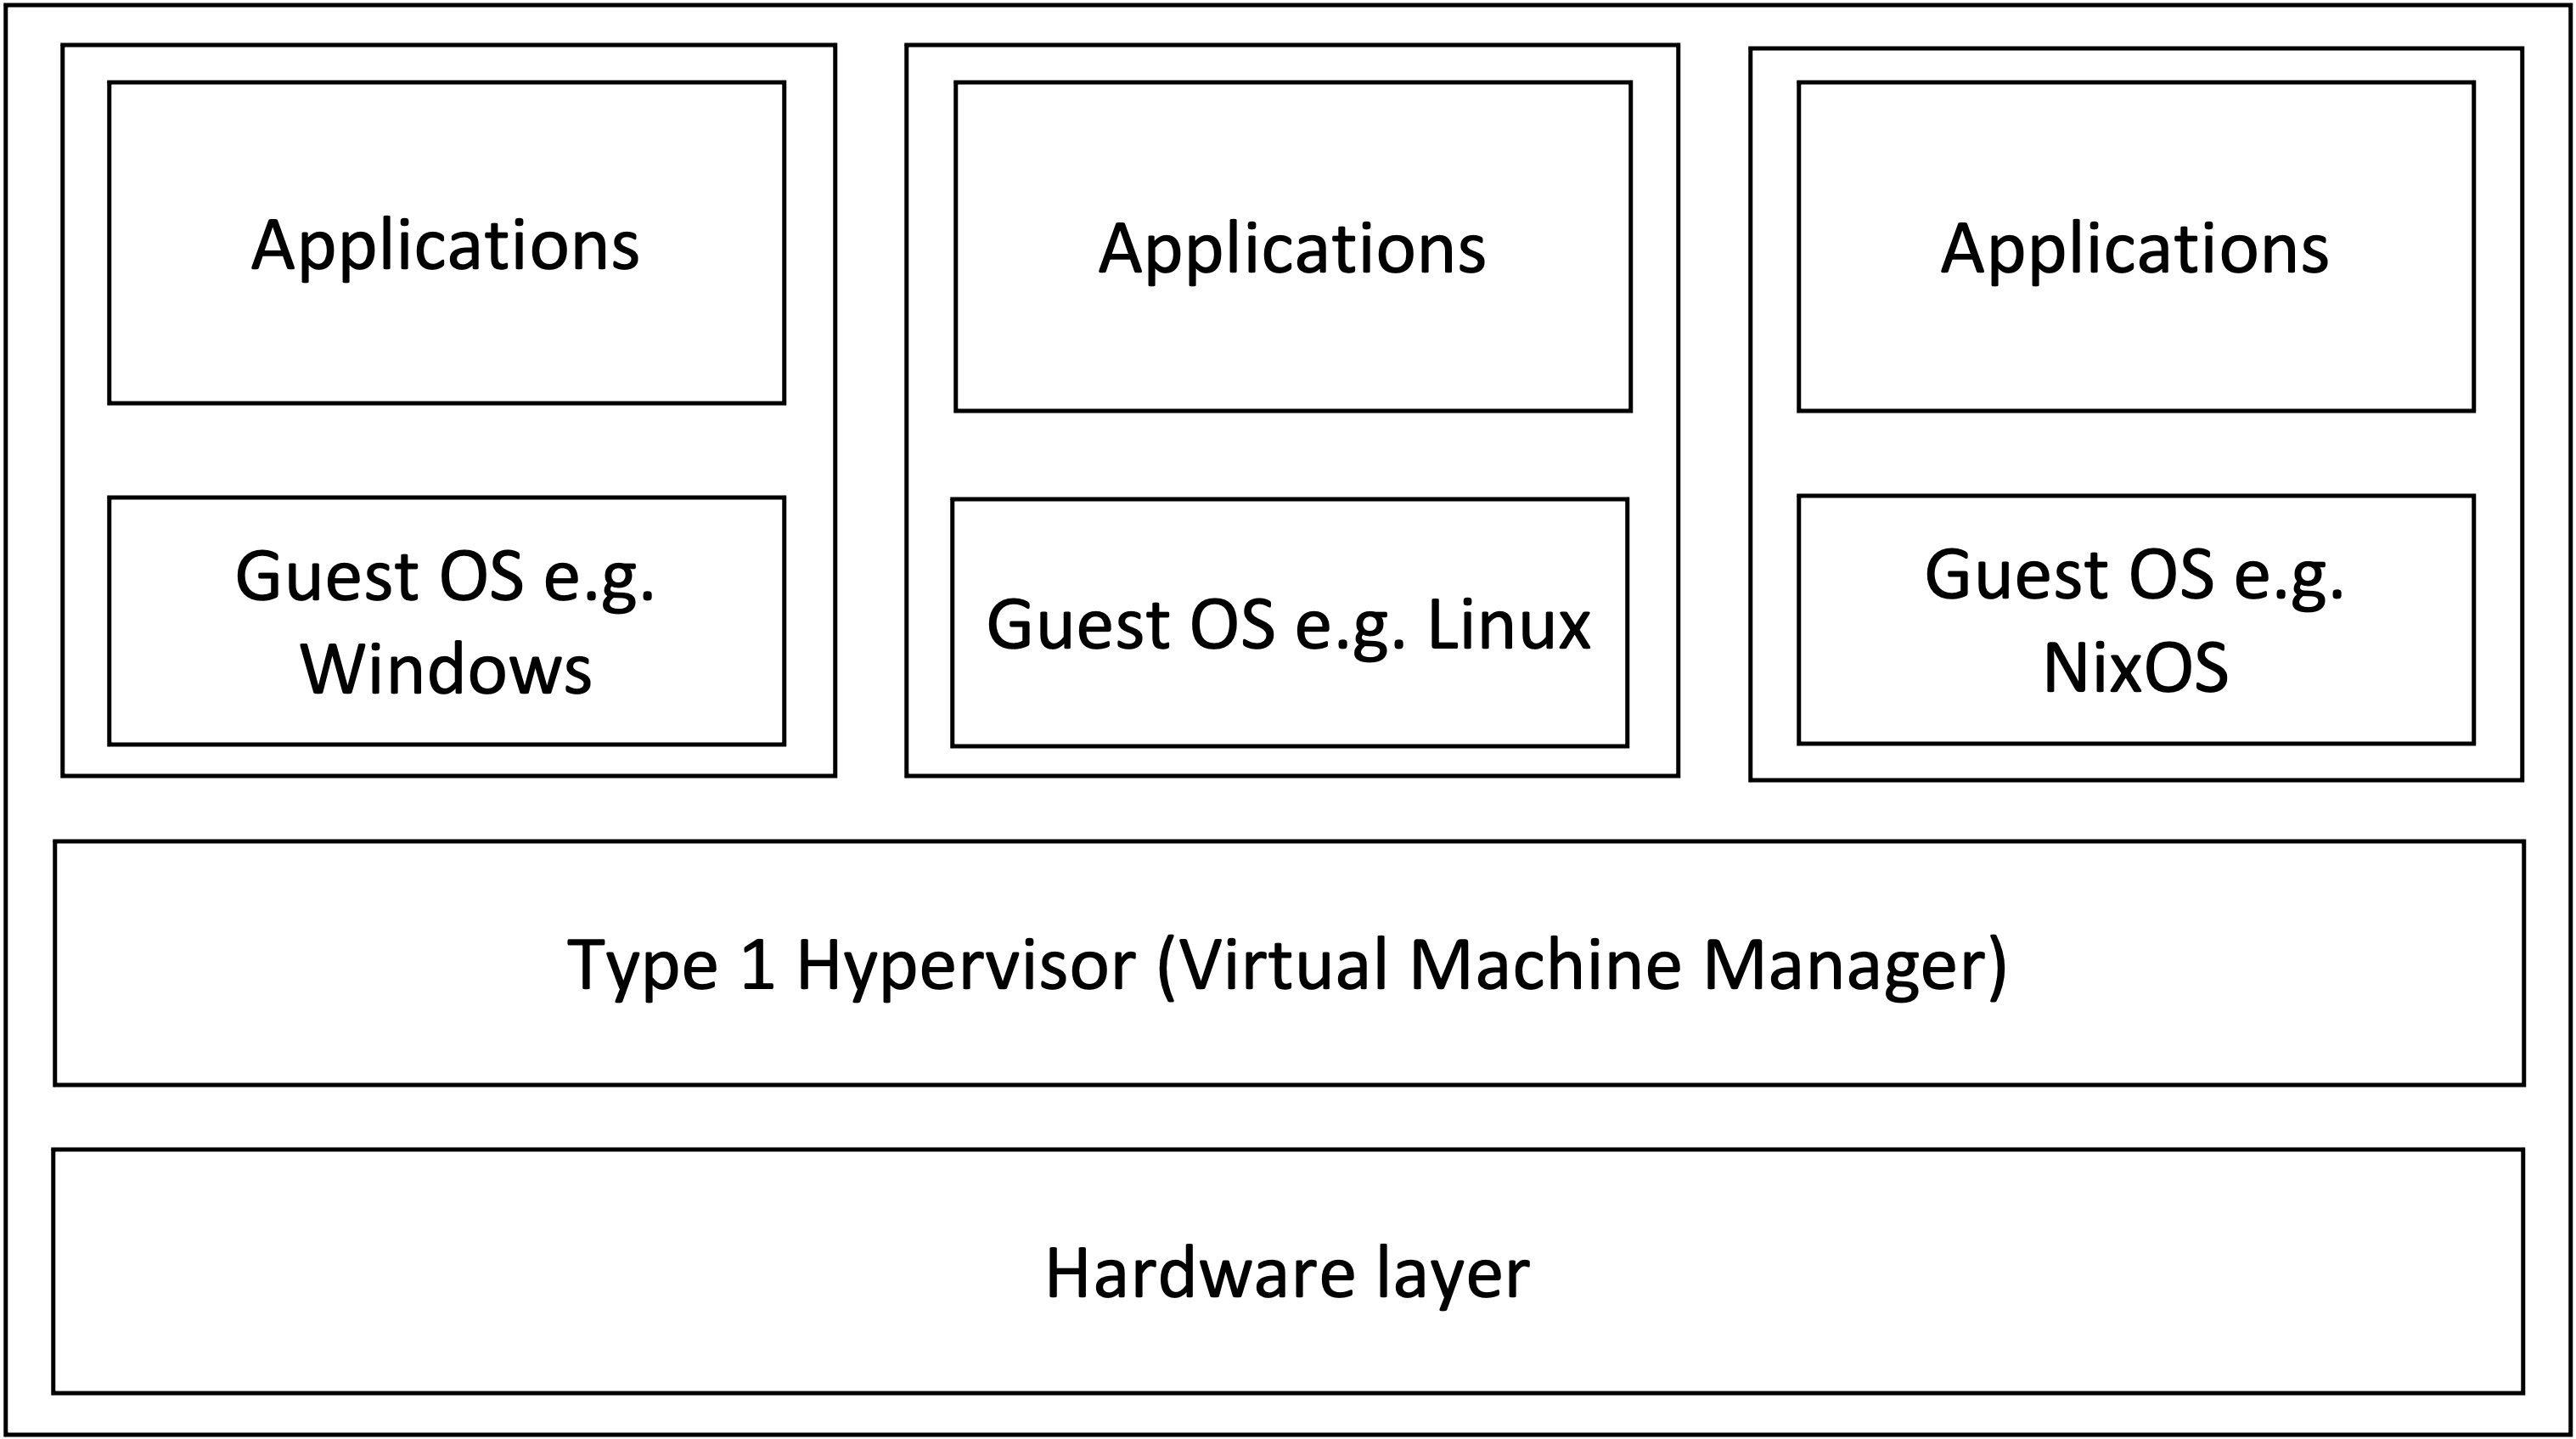
\includegraphics[width=\textwidth]{thesis/graphics/hardware-layer-virtualization.png} 
\caption{Hardware-layer virtualization or type 1 hypervisor}
\label{fig:Hypervisor-type-1}
\end{subfigure}
\begin{subfigure}[t]{0.49\textwidth}
\centering
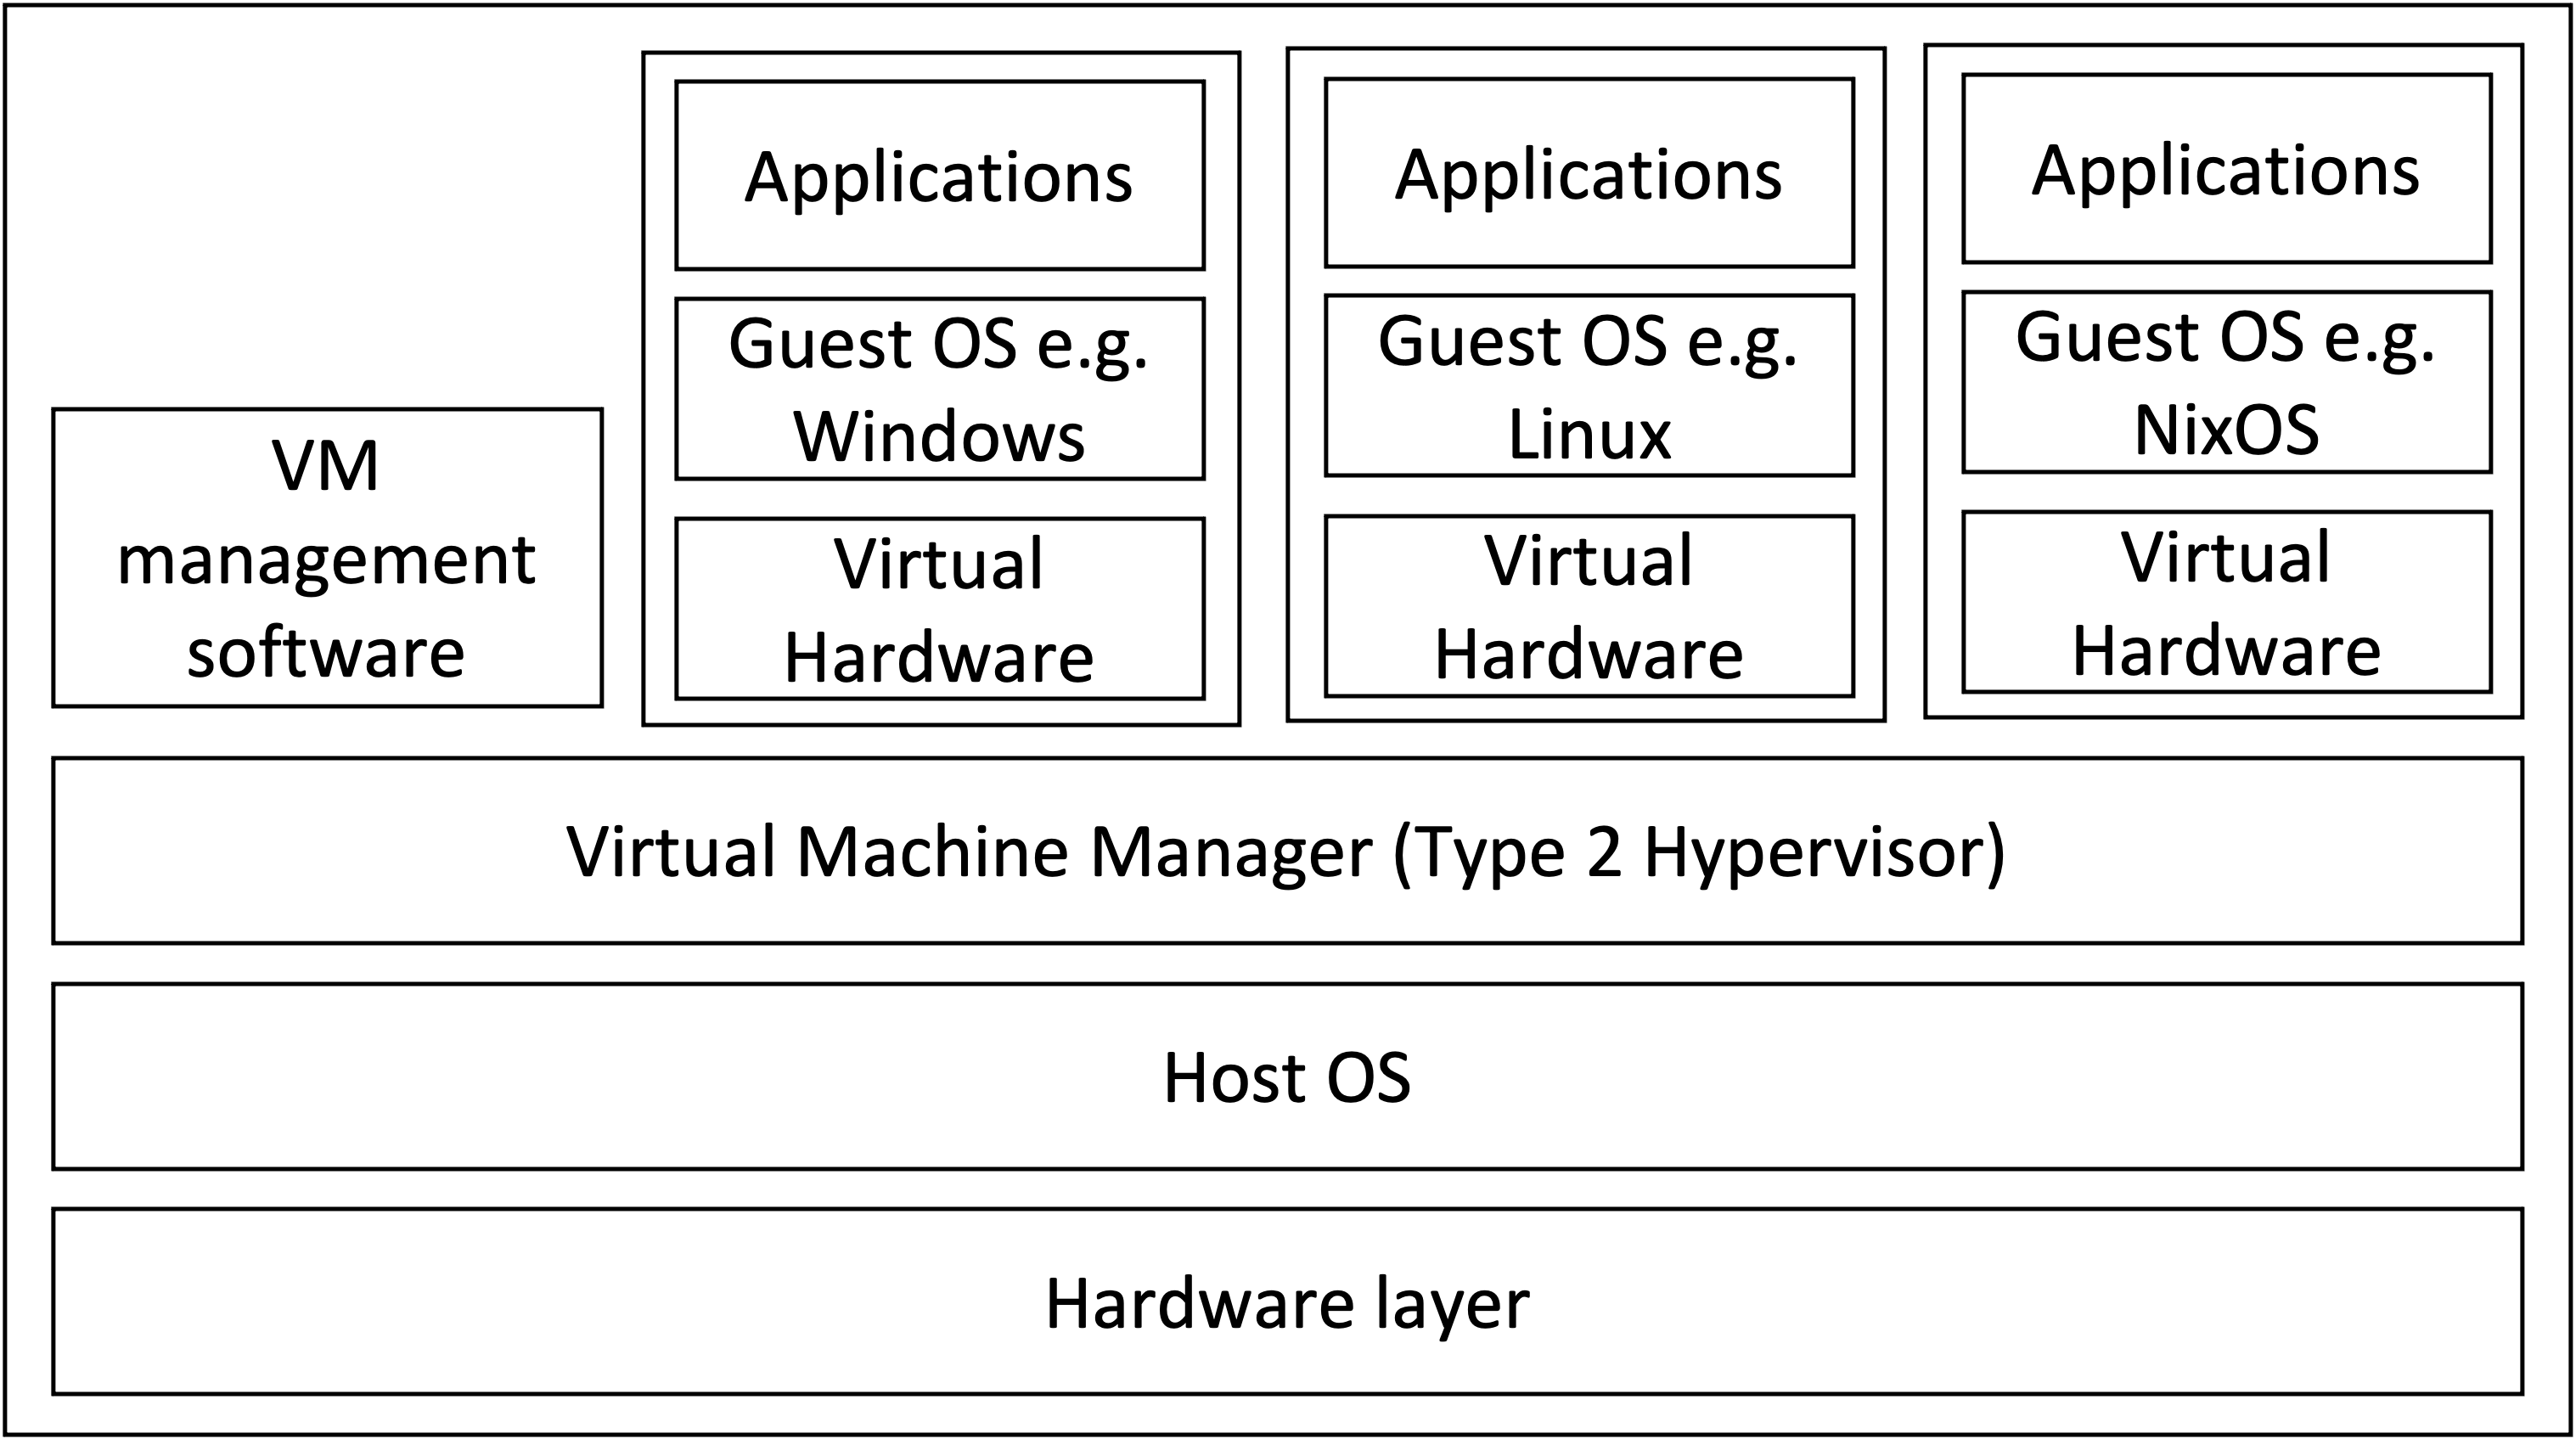
\includegraphics[width=\textwidth]{thesis/graphics/full-virtualization.png}
\caption{Full virtualization or type 2 hypervisor}
\label{fig:Hypervisor-type-2}
\end{subfigure}

\caption{Different types of hypervisor-based virtualization architectures (adapted from \cite{Sahoo2010}).}
\label{fig:Virtualization}
\end{figure}

\subsection{Container-based OS-layer virtualization}\label{OS-layer-virtualization}
Containers share some characteristics with VMs but are an example of \emph{OS-level virtualization}. OS-level virtualization, represented by the \emph{virtualization layer} -- also known as \emph{container engine}, virtualizes a single host OS to provide the illusion of multiple instances or ``containers'' of that same OS (see fig. \ref{fig:OS-Layer-virtualization}). Unlike hypervisors, each container is constrained to run the same OS as the host. This means that the host’s kernel is shared, and applications can safely share system libraries and executables across containers rather than having possibly redundant copies in each VM. Multiple containers can be run in parallel, and each can be started, stopped, and removed by the container engine. The ability of containers to share resources with the host OS and share data with other containers makes them efficient \cite{Mouat99117185791205503}\cite{redHatContainerTerms}. 
%Containers are an encapsulation of an application with its dependencies.

OS-level virtualization achieves isolation by limiting the \emph{filesystem namespace} and the \emph{process namespace}. The process namespace binds a process to its execution environment. The filesystem namespace refers to the organization of the bindings between names and files. The filesystem namespace can be limited by changing the root for each container. The process namespace is limited, so processes can only ``see'' other processes that share their container. The OS or virtualization layer may provide more sophisticated scheduling and memory allocation policies for running containers instead of standard processes. How this is done exactly is out of the scope of this thesis. 

A privileged container (see fig \ref{fig:OS-Layer-virtualization}) exists in this system that provides an interface to the virtualization layer. This allows a system administrator to manage other containers and assign resources to containers at the time of creation or dynamically at runtime. These resources could include disk space, CPU guarantees, and memory limits. To applications and the user of a container-based system, the container appears just like a separate host. Processes running inside the container are native processes on the host with the same system call interface as the underlying host OS \cite{Soltesz2007}\cite{Mouat99117185791205503}. 
\begin{figure}
  \centering
  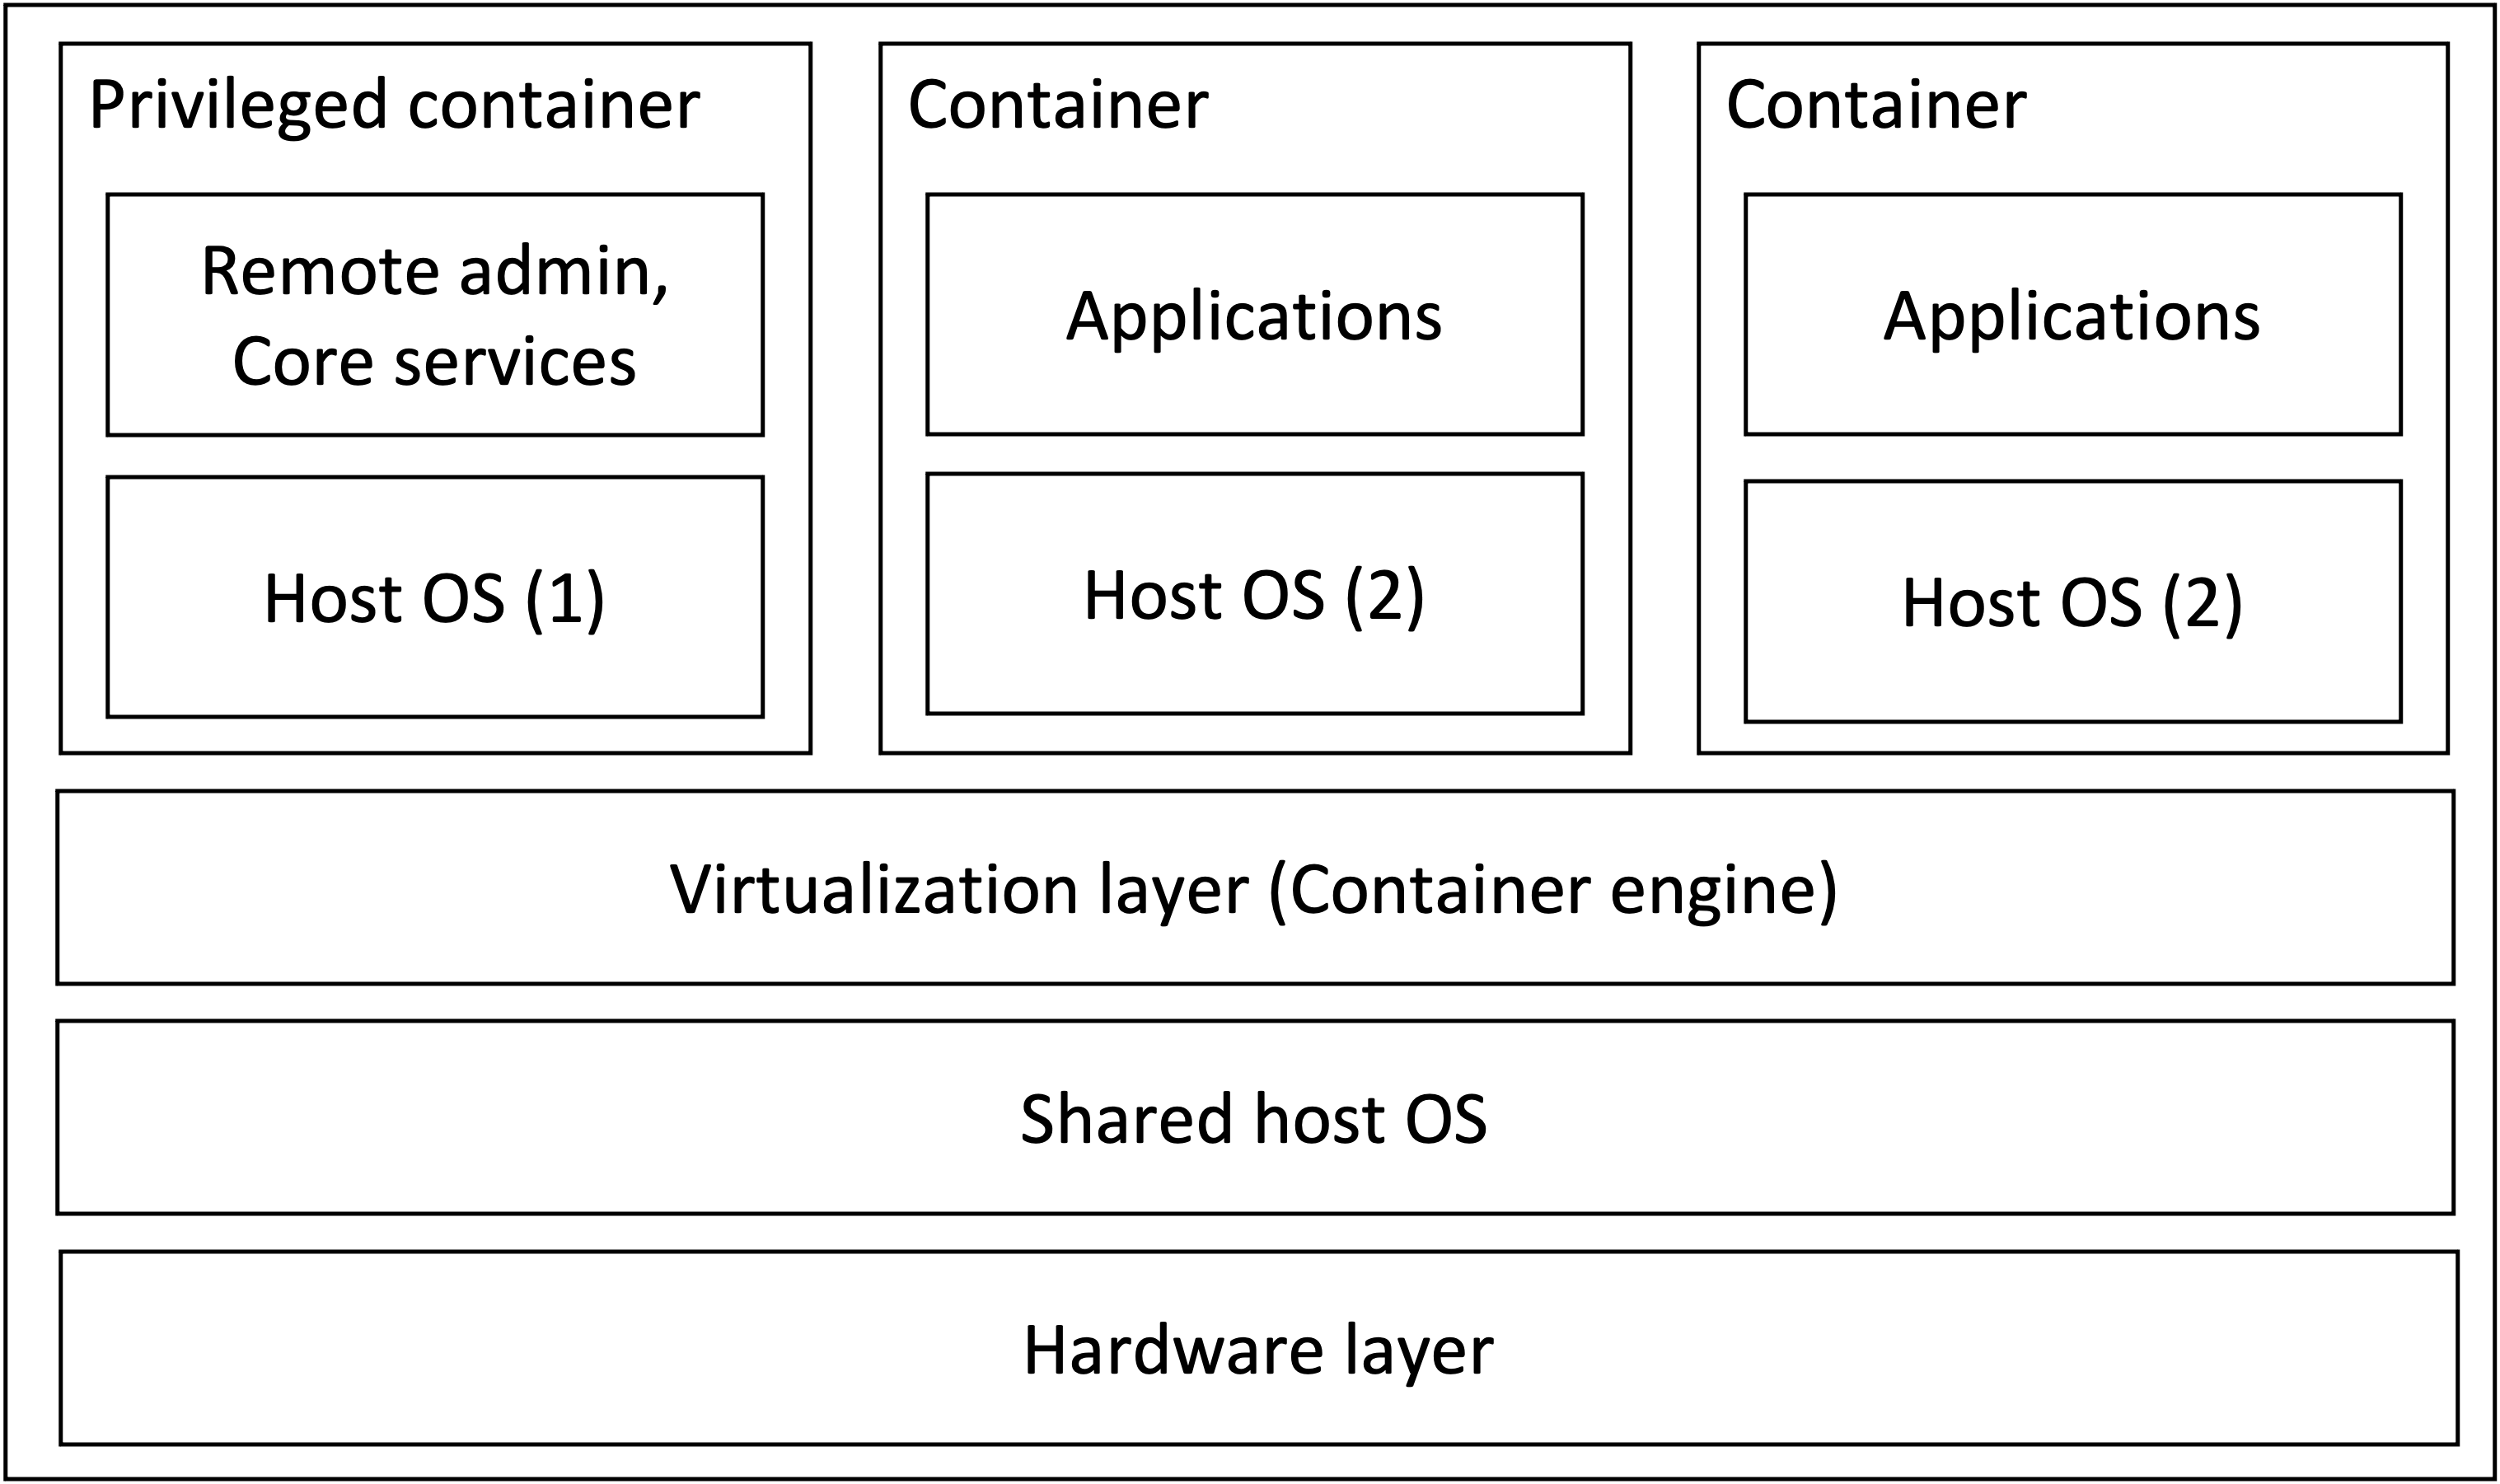
\includegraphics[width=0.7\textwidth]{thesis/graphics/OS-layer-virtualization.png}
  \caption{OS-Layer virtualization architecture overview as the basis of containers (adapted from \cite{Sahoo2010}).}
  \label{fig:OS-Layer-virtualization}
\end{figure}

\subsection{Containers versus VMs}\label{containers-vs-VM}
Containers and VMs can both be used to isolate applications from each other running on the same hardware. They are commonly used to achieve different goals -- containers are used to make applications \emph{self-contained} and \emph{portable}, while the purpose of VMs is to emulate a system entirely. Self-contained means that the application does not rely on dependencies external to the container. Portability is hiding the details of an application's execution environment to transfer it to another platform effortlessly. A platform includes hardware, the OS, system users, and software interfaces. Containers are somewhat limited in functionality compared with VMs, but they enable use cases that are difficult to achieve with VMs \cite{Mouat99117185791205503}. 

The self-containment and portability properties of containers have advantages in cloud deployment and for developers who can download images and run containers without worrying about configuration, differences in user environments, and installing dependencies \cite{Mouat99117185791205503}. Containers can be started and stopped in a fraction of a second. Processes of containers do not incur the overheads of hypervisor execution (e.g., interpreting system calls). The sharing property of a container system makes containers more efficient (``lightweight'') compared to VMs. This results in system administrators being able to run many more containers on a single host machine than VMs. 

Research confirms the above claim that containers tend to be more efficient and suggests that they guarantee almost the same resource isolation as VMs (at present; some researchers dispute both claims) \cite{Soltesz2007}. However, hypervisors are a trusted and battle-tested technology, whereas containers are comparatively new, resulting in companies not fully trusting the isolation of containers. This lack of trust has led to hybrid systems with containers running inside VMs to take advantage of both technologies \cite{Mouat99117185791205503}. 

\section{Containers}
Containers are an old idea, where a basic form of system-level virtualization was introduced to FreeBSD in 1998. Then in 2008, the Linux Containers project (LXC) started and brought together system-level virtualization and resource limiting for memory and CPU. The result was a complete containerization solution. The final piece to the containerization ecosystem was brought by Docker in 2013 and enabled widespread adoption of the technology by companies like Red Hat, Microsoft, and Amazon and the developer community. Docker extended existing Linux container technology (i.e., LXC) with a standard container format to allow portable images. It also added a user-friendly interface and tools to build, run and distribute containers \cite{Mouat99117185791205503}. 

The different available container solutions, each having a different container image format, and the rise of Docker led to the development of an independent formal standard for the container runtime and image format. This standard is known as \emph{OCI Image Specification} after the governance structure Open Container Initiative (OCI) that created it. The OCI Image Specification was based on the original Docker image format and is adopted today by almost all major container engines and tools. LXC and many other container engines and container orchestration options exist, such as OpenVZ and Kubernetes, but Docker remains the industry standard containerization software \cite{Mouat99117185791205503}. 

This section introduces essential concepts of a container system used in this thesis. The theoretical and abstract view of such a system was introduced in \ref{OS-layer-virtualization}  Since the current CodeExpert approach and our prototypes use Docker, we will use it in the following as an example for some of the more general containerization concepts.

\subsection{Container image}\label{container-image}
%When we use the term \emph{container image} in this thesis, we mean images in the OCI image format. This format defines a container image as a collection of multiple tar files (one file for each \emph{layer}) and a \emph{configuration file} \cite{redHatContainerTerms}. 
Container images are already introduced in definition \ref{def:container-image}. %The configuration file contains image metadata, which provides extra information about the layers, and an ordered list of layer references -- not the actual files of each layer \cite{BraunDockerLayers}.
An image often extends another image, called the \emph{base image}, with some additional customization, i.e., software packages necessary for running one's application. Images are then used to store one's application and deploy it to a server. In the case of Docker, the instructions defining the steps needed to build the image and run it are written with a \verb|Dockerfile| \cite{dockerOverview}.

\subsection{Container}\label{containers}
%A \emph{container} has two states (resting and running), similar to the states of a process. In the rest state, it is a set of files and metadata (i.e., the container image) saved on a disk. When one starts a container, the container engine creates a runtime instantiation of the container image. In particular, the container engine unpacks the set of files and metadata and makes a system call to the kernel to start a process. This system call initiates extra isolation (see \ref{OS-layer-virtualization}) and mounts (i.e., makes available to users) a copy of the container image files. Now the container is in the running state as a Linux process. 
A container has been defined in \ref{def:container}, and some other important properties are introduced next. Typically, configuration options can be added to a container when starting it, like limiting the memory capacity or setting environment variables. Thus a running container is defined by the container image used as a mount point to start it and the provided configuration options \cite{redHatContainerTerms}. One can connect a container to subsystems such as network or persistent storage (introduced in \ref{container-storage}) and control the degree of isolation of each container from other containers and the host machine. The container life-cycle ends when removing a stopped container and any state not stored in persistent storage or the image's layers at build time disappears \cite{dockerOverview}. 

\subsection{Image layers}\label{layers}
We need to know how layers are created, stored, and cached to understand the uses and performance aspects of images and containers. In this section, we will use Docker as an example to explain the relation between images and layers and the connection between containers and layers.

\paragraph{Images and layers}\label{images-and-layers}
Recall from definition \ref{def:container-image} that container images are a collection of layers. Layers in an image relate to each other through a parent-child relationship. The union of all layers comprises the content of an image. Each image layer represents the changes between itself and the parent layer. Each parent layer contains the set of differences (\verb|diff|) to the filesystem of the child layer. %In the case of Docker, the instructions in a \verb|Dockerfile| specify how an image is built. %All other instructions in a \verb|Dockerfile| only change the image's metadata and do not produce a new layer. 
For example, in the case of Docker, if a \verb|Dockerfile| instruction copies a file into the image's filesystem, this file is located in the \verb|diff| of a layer \cite{DockerStorageDrivers}\cite{BraunDockerLayers}. Each layer is identified by a \emph{content addressable ID} that is the hash value of its content \cite{BraunDockerLayers}. A content addressable store is analogous to the concept of \emph{content addressable memory} that `refers to a principle of organization and/or management of memories [...], or searching of data on the basis of their contents rather than by their location \cite[p.~1]{Kohonen1980}.' The modifications of the \verb|Dockerfile| that result in changes of the \verb|diff| of a layer are cached as a separate layer cache. A container image is built by progressively merging the files inside the layers on top of the base image. The cached layer is used whenever possible during the merging. The merging of layers is possible due to the \emph{union filesystem} that Docker uses that allows stacking multiple filesystems or directories to appear as a single filesystem \cite{DockerStorageDrivers}\cite{Wright2004}.

The two primary advantages of constructing images and layers in this format are efficient storage usage and faster rebuilds. The separation of the image configuration file from the files that store the contents of the layers allows sharing layers among multiple image configurations by referencing the same layer. Thus, for example, if multiple images use the same base image, then the layers of the base image have to be stored only once on disk resulting in efficient disk usage \cite{DockerStorageDrivers}.
The cached layers avoid recomputations in an image rebuild after a configuration change. Specifically, almost only those changed layers are rebuilt, resulting in faster image builds \cite{dockerOverview}.
%In the case of Docker, each layer has its own directory within Docker's storage directory that contains, among others, the \verb|diff| and the \verb|cache-id|. Each layer has an associated cache, which is identified by the hash value of the cache (the \verb|cache-id|). Just as with layers, Docker stores all cached layers in directories that correspond to the cache ID. Cache directories contain a subdirectory called \verb|diff|, representing the modification to the filesystem \cite{BraunDockerLayers}. 

\paragraph{Containers and layers}\label{containers-and-layers}
When a new container is started, a new writable layer is added on top of the read-only layers. This writable layer is the significant difference between a container and an image and is why it is often called the ``container'' layer. This layer allows some write access to containers, as all changes made to the running container, such as writing, modifying, or deleting files, are written to this thin container layer. To achieve this, Docker utilizes a \emph{copy-on-write} mechanism that copies a file from some read-only layer to the writable layer if the container updates the file for the first time. This mechanism implies that containers that write a lot of data, which the copy-on-write mechanism writes to the writable layer, consume more space than those that do not. When a container is deleted, the writable layer disappears, and the underlying image remains unchanged \cite{DockerStorageDrivers}. The copy-on-write mechanism helps to make containers efficient. It saves space, as the read-only layers can be shared among containers. Additionally, it reduces container start-up time, as the container engine only needs to create the container layer \cite{DockerStorageDrivers}.
\begin{figure}[h!]
  \centering
  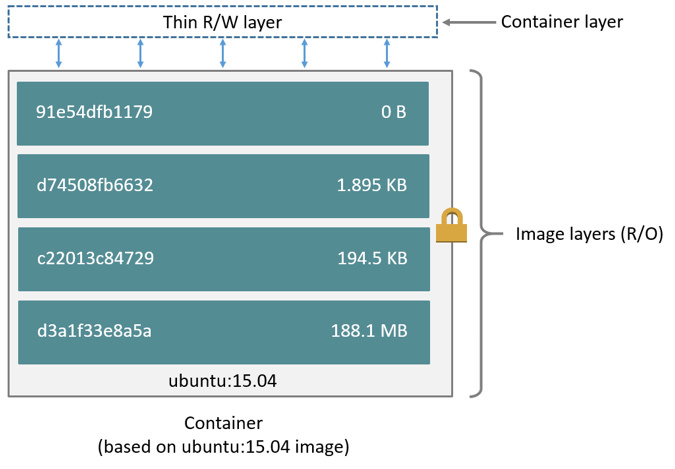
\includegraphics[width=\textwidth]{thesis/graphics/container-layers.jpg}
  \caption{Docker container layers based on ubuntu:15.04 image. R/W means that the container can read and write to this layer. Each read-only (R/O) layer is represented by its content-addressable hash and size of the layer \cite{DockerStorageDrivers}.}
  \label{fig:container-layers}
\end{figure}

\subsection{Image registry}
A \emph{image registry} is a repository, typically run as a server, for storing images. If the container engine does not have a locally cached copy of the container image, it will automatically try to download (``pull'') it from an image registry server. It is also possible to upload (``push'') a locally built image to an image registry. One can configure the registries the container engine will use to pull images from -- Docker uses, by default, the public registry called Docker Hub. It is also possible to run a private registry instance for example in a container \cite{dockerOverview}\cite{redHatContainerTerms}. 

\subsection{Storage}\label{container-storage}
The following section provides an overview of standard persistent storage options that can be attached as a subsystem to a container. For this section, we use the documentation of Docker, but the different storage types apply to other containerization options. Our prototype uses some introduced storage options to persist data across the container life-cycle. 

This thesis uses two storage types: volumes and bind-mounts. We can visualize their differences by looking at where the data is stored on the host machine (see figure \ref{fig:docker-storage-overview}). Another common storage type (tmpfs mounts) is out of the scope of this work.
\begin{figure}[h!]
  \centering
  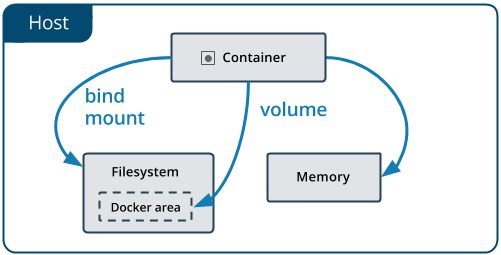
\includegraphics[width=0.7\textwidth]{thesis/graphics/types-of-mounts.png}
  \caption{Location of where the data of volumes and bind mounts is stored on the host machine (adapted from \cite{DockerStorage}).}
  \label{fig:docker-storage-overview}
\end{figure}
\paragraph{Volumes}
\emph{Volumes} facilitate persistent data storage that can be shared safely across multiple containers. New volumes can have their content prepopulated by a container. Volumes are often chosen over persisting data in a containers writable layer (see \ref{containers-and-layers}). The reason is that a volume does not increase the size of the containers using it and the data stored in the volume exists outside the life-cycle of a container. In the case of Docker, a volume is stored in a directory within Docker`s storage directory on the host machine, and Docker manages a volume by managing that directory`s contents (see fig. \ref{fig:docker-storage-overview}) \cite{DockerVolumes}\cite{DockerBindMounts}. 
\paragraph{Bind mounts}
When using a \emph{bind mount}, a file or directory -- specified by an absolute path -- on the host machine is mounted into a container. The bind mounts may be stored anywhere in the filesystem of the host and can be modified by processes inside the container and on the host (see fig. \ref{fig:docker-storage-overview}) \cite{DockerStorage}. Bind mounts have limited functionality and are much less performant on Windows or Mac hosts compared to volumes \cite{DockerBindMounts}\cite{DockerVolumes}. Nonetheless, they help mount a small number of specific files into a container and are very performant on Linux hosts, provided that the host has the right filesystem directory structure \cite{DockerBindMounts}.
%\paragraph{tmpfs mounts}
%This storage option is useful to temporarily store sensitive files that one does not want to store in the host filesystem or the container's writable layer. Unlike bind mounts or volumes, a \verb|tmpfs| mounts are temporary and persist data in the host memory (see fig. \ref{fig:docker-storage-overview}). Once the container stops, the \verb|tmpfs| mount is removed, and the files written in the mounts memory area are deleted \cite{DockerTmpfsMount}. 

The containerization concepts from this chapter and the virtualization chapter form the basis for the next chapter on cloud-based integrated development environments that often use containers to execute users' code remotely.

\section{Cloud-based integrated development environments}\label{cloud-based-IDE}
This section introduces cloud-based IDEs and their difference from traditional IDEs. Additionally, we cover the implications of a cloud-based IDE on how a programming environment should be set up.

Traditional Integrated Development Environments (IDEs) accelerate software development by providing an effective way to browse and manipulate a system's source code as opposed to using a plain text editor and command line \cite{BruchBodden2010} \cite{FYLAKTOPOULOS2018127}. A traditional IDE provides developers with a development environment where the IDE is commonly responsible for tasks such as dependency management, debugging, and auto-completion \cite{Applis2019}. Popular IDEs include Microsoft Visual Studio, Eclipse, and NetBeans.

A cloud-based IDE is run in a cloud computing system, and developers can access the IDE from any web browser at any time \cite{Yanagisawa6354897}. Compared to a traditional IDE, which must be installed before using it, each developer does not have to install dependencies and compilers on the local system. Cloud IDEs set up a shared workspace, which is shared among the programmers. Furthermore, they provide a large pool of computing resources for development to support developer collaboration. Popular cloud-based IDEs include CodeSpaces, Cloud9, Replit, and Eclipse Che. 

A cloud IDE should offer programming languages as runtime execution environments as developers may want to use different programming languages. These environments are often executed inside containers, making them cloud-native applications. Furthermore, a standard runtime environment configuration can be shared among developers \cite{Applis2019}\cite{FYLAKTOPOULOS2018127}.

\section{CodeExpert}\label{CodeExpert}
Since this thesis compares its results to the current implementation of \emph{CodeExpert} and discusses its tradeoffs, we need to understand its architecture and general workflow.

\subsection{Architecture}
CodeExpert is a cloud-based IDE developed at ETH Zürich that is used to enhance computer science studies and programming classes. The architecture consists of four primary services, split into the front-end (\emph{cxweb}) and the back-end. The back-end includes the database, back-end runner (\emph{cxrun}), and image registry (see fig. \ref{fig:cx-architecture}). The CodeExpert IDE is accessed via web browser and executed inside containers.
\begin{figure}
   \centering
   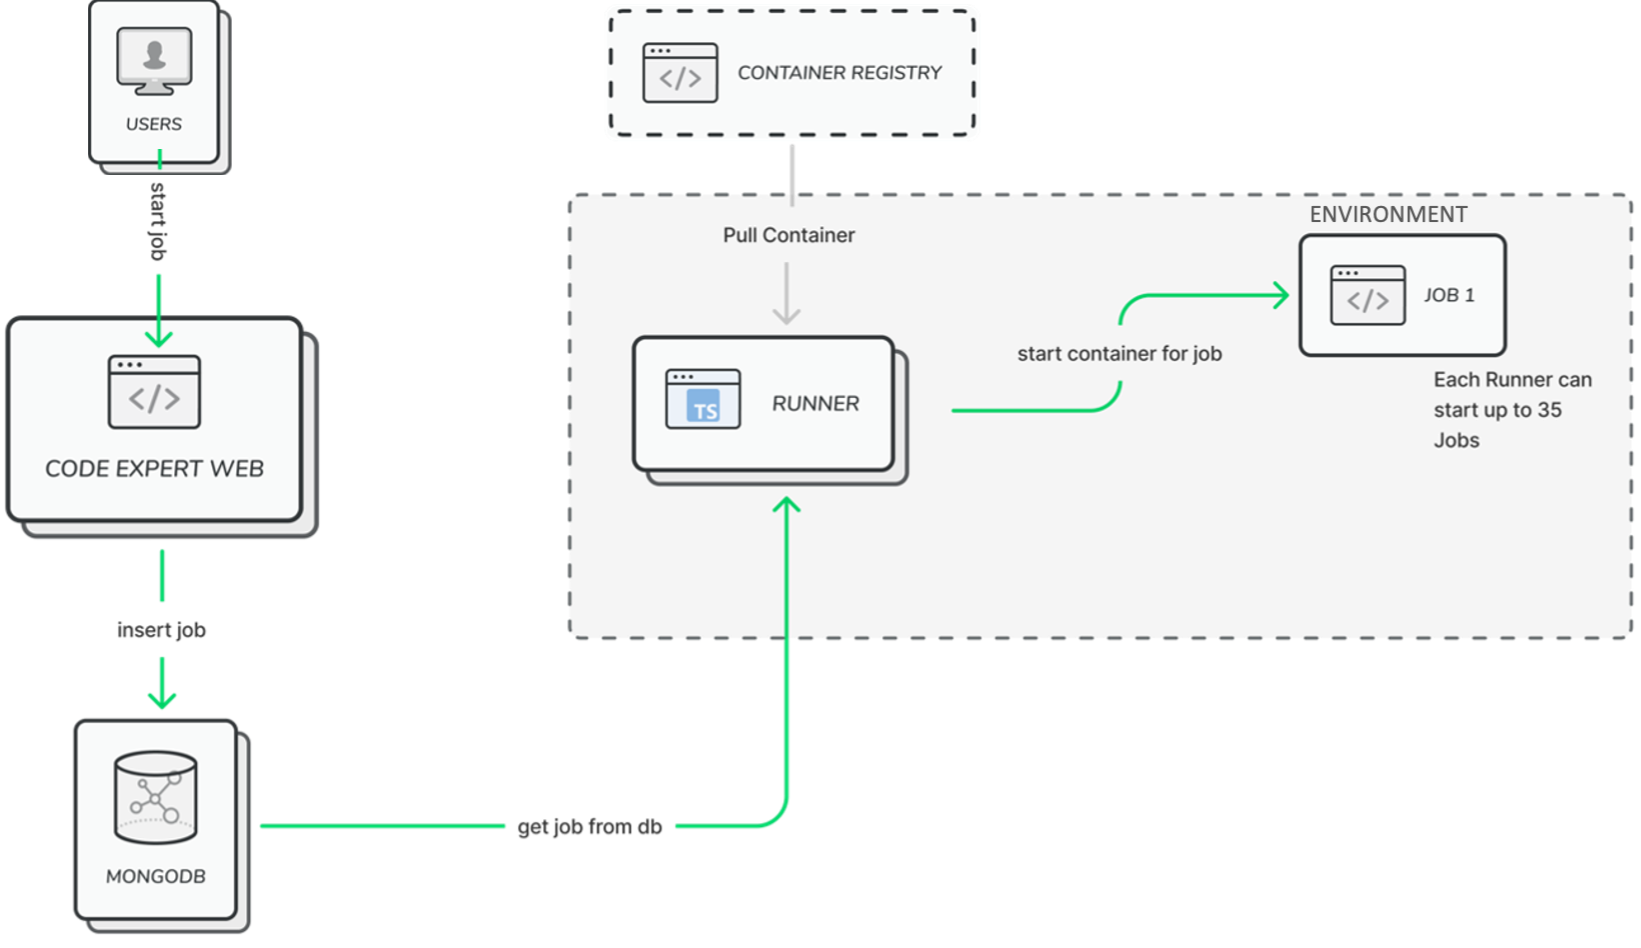
\includegraphics[width=\textwidth]{thesis/graphics/CodeExpertArchitecture.png}
   \caption{CodeExpert architecture and job execution flow (adapted from \cite{CodeExpertTechnicalOverview})} 
   \label{fig:cx-architecture}
\end{figure}
The front-end is separated from the back-end through interfaces. Each service is running on multiple different virtual machines. This decoupling of the front-end from the back-end allows the system to scale -- as the workload increases -- the back-end and front-end services independently. 

\subsection{Execution flow}\label{CX-execution-flow}
For each interaction (e.g., executing or compiling code) of the student, cxrun starts a new cloud-native environment (\emph{cxEnvironment}) in which the code is executed remotely. After the execution has terminated, the container is removed, and the execution output is redirected by cxrun to cxweb. This allows the student to inspect the output \cite{CXDocs}. 

\subsection{Configuration}\label{CX-configuration}
The lecturer explicitly specifies the cxEnvironment for each project, and the lecturer can use predefined cxEnvironments for programming languages such as \verb|C|/\verb|C++|, \verb|Python|, and \verb|Java|. Lecturers can also define a custom cxEnvironment using a \verb|Dockerfile|, which is then built to an image and pushed to the image registry (denoted as ``container registry'' in fig. \ref{fig:cx-architecture}). The image registry runs in a container inside the local network. The building and pushing are done at build time before the custom image can be used as runtime environment \cite{CXDocs}.

\section{Build system}
After our discussion on cloud-based IDEs and CodeExpert, this section will introduce some properties and tools of a \emph{build system} that we will use to build images at runtime. 

\subsection{Reproducibility}\label{reproducibility}
Coding environments that lectures use for their student should be \emph{reproducible}, as they are, for example, used in exams. Reproducibility of environments means building the same configuration twice should yield the same environment. To achieve reproducibility, we must manage software versions and dependencies and manage development environments. The latter is commonly handled with containers (e.g., Docker) and VMs that provide controlled environments in which the user code can be executed \cite{bedo2010}. 

We have already learned that a container image allows reproducible containers (see definition \ref{def:container}). However, the Docker image build system does not guarantee reproducible images. When building images twice from the same \verb|Dockerfile|, one might get two images that behave differently. The different behaving images could break the user's runtime environment. This non-determinism happens, for example, when a third-party package dependency gets silently updated or when the package version is not specified (``pinned'') when writing the \verb|Dockerfile|. The silent update results from non-purely-functional package managers (a concept explained in \ref{Nix-theory}), whereas not pinning the package version is a terrible practice. Pinning all package versions helps, but there are many details to consider, and it does not relieve the issue completely \cite{OHearn}.

The non-reproducibility issues of building images with \verb|Dockerfile|'s motivate the use of a purely functional package manager and a system to build the coding environment, called a \emph{hermetic} build system. Given the same input source code and configuration, this system returns the same output using isolation and \emph{source identity}. This is the topic of the next section.

\subsection{Hermeticity}\label{hermeticity}
A \emph{hermetic} build system isolates the build from the underlying host system. Thus a hermetic build is insensitive to libraries and software installed on the host machine and depends only on specific versions of build tools (e.g., compilers) and dependencies (e.g., libraries). The result is self-contained builds \cite{HermeticityBazel}. 

A hermetic build tries to ensure the consistency and sameness of inputs, a concept called source identity. Source identity is achieved with the help of code repositories, such as Git, where the unique hash code that identifies code mutations is used to track changes to the build's input. More specifically, isolation between the host machine and the user is achieved by downloading copies of tools and managing their storage inside managed file trees \cite{HermeticityBazel}. 

The benefits of having a hermetic build system are speed, multiple parallel builds, and having multiple versions of the same package coexist. Builds can be cached unless the inputs change, resulting in fast builds. Parallel builds can be executed by computing the graph of actions to take such that the output is built from the input. As the storage of the packages is managed by the hermetic system, we can easily use different versions of tools in multiple builds without colliding installation paths. Thus, we do not need to create a different container environment for different package versions \cite{HermeticityBazel}\cite{NixPills1}. Furthermore, a hermetic build system implies reproducibility \cite{HermeticityBazel}. Since the build output does not depend on anything outside the build, we can copy it across different systems and potentially make it portable.

\subsection{Package manager}
Software platforms strive to provide modular software components, called software \emph{packages} that can be assembled to provide the user with the desired functionalities. A package is an archive file containing a program and necessary metadata. The program can be in \emph{source code} that must be compiled and built first. The metadata may include, among others, the package version and description and requirements for relationships (e.g., versions) to other packages and the target system. Installing more than one copy of a package on a given system is impossible. Packages cannot be composed to build a larger component, and they may conflict with each other. The latter can happen because the installation and execution of packages act on shared resources provided by the OS, like creating files or interacting through the systems input/output devices. The essential tools for managing software versions and their dependencies (installing, upgrading, and removing packages) are \emph{package managers}. They allow to retrieve packages from central (remote) repositories and check their integrity. Furthermore, they resolve conflicts between package requirements and provide tools to manage the installation on a user's system. Resolving requirements conflicts is a functionality known as \emph{dependency solving} and is introduced next \cite{ABATE2013459}\cite{bedo2010}. 

\subsection{Dependency management}
\emph{Dependency management} is usually specific to your OS, programming language, or application and is either done by an IDE (see \ref{cloud-based-IDE}) or by a separate package manager. Some examples of popular package managers include \verb|dpkg| for Linux and \verb|Conda| or \verb|pip| for the \verb|Python| language. Traditionally the IDE or package manager installs dependencies on one's local machine to set up a development environment. Thus a cloud-based IDE also needs to handle dependency management for setting up the correct runtime environment. The offloading of dependency management and maintenance to the cloud IDE relieves the developer from the burden of setup, configuring, and upgrading their environments \cite{Yanagisawa6354897}. 

\section{Nix}\label{Nix-theory}
In this thesis, we use Nix as a container image build system that includes a purely functional package manager to achieve reproducible development environments that are hermetically built. Being functional means that a build has no side effects -- building a package twice with the same inputs yields the same output. This property enables Nix to compose environments at runtime easily. This is unlike many widely used package managers such as \verb|dpkg|, \verb|rpm|, which are not purely functional and mutate the global state (write to \verb|/bin|, \verb|/usr|, and \verb|/etc|) of the system during package management operations \cite{NixPills1}\cite{vanDerBurg2012}.

Nix provides multiple tools to make builds reproducible. The first is a purely functional domain-specific language called Nix. Second, it provides a Nix store that safely stores multiple versions and variants of packages next to each other. Furthermore, it features atomic upgrades and rollbacks of package versions and builds and a garbage collector, among others \cite{vanDerBurg2012}. %We will interchangeably use the term Nix to refer to the image build system, language, and package manager. 

\subsection{Derivations}\label{Nix-derivations}
Nix stores all packages in isolation and as immutable file system objects (i.e., files and directories) in the Nix store. Packages or software components are build outputs referred to as \emph{derivations} inside Nix. Derivations are built from declarative specifications, called \emph{Nix expressions}, written in the Nix language. They describe all inputs such as sources, build script, and environment variables that go into a package build action. Each build action first constructs an isolated environment with all the inputs needed to run the build script and then executes this script to run all the build steps \cite{vanDerBurg2012}\cite{NixPills1}. All inputs, dependencies, and steps of a build process can be represented as a dependency graph, called \emph{closure}. This graph has build actions as its nodes \cite{NixPills3}. Nix can construct a new reproducible environment with additional packages by adding new nodes to the closure. Nix ensures a high degree of reproducibility of each Nix expression by removing many side effects such as limiting network and filesystem access and building in an isolated (``sandboxed'') container. Additionally, it clears all environment variables and patches build tools (such as \verb|GCC|) to ensure that they do not mutate the global filesystem \cite{vanDerBurg2012}. 

Every derivation has a unique subdirectory \verb|g32imf6...-firefox-1.0.1| in the Nix store (see fig. \ref{fig:nix-user-environments}) where part of the name \verb|g32imf6...| is a cryptographic hash code of the packages build dependency graph (closure). The closure captures all dependencies and versions of a package. A cryptographic hash of the closure is used so that different versions of dependencies result in different hash codes. This implies that it is safe to install different versions without conflicts \cite{vanDerBurg2012}. This mechanism is the basis of the Nix stores content addressability feature. 
Nix expressions describe how to build derivations from source code, which can take a long time, as potentially all dependencies in the dependency graph need to be built. To avoid this, Nix skips building from source code if the corresponding derivation is available in a binary cache. By default, Nix downloads pre-built binaries from cache.nixos.org \cite{NixPills1}.
\begin{figure}[h!]
  \centering
  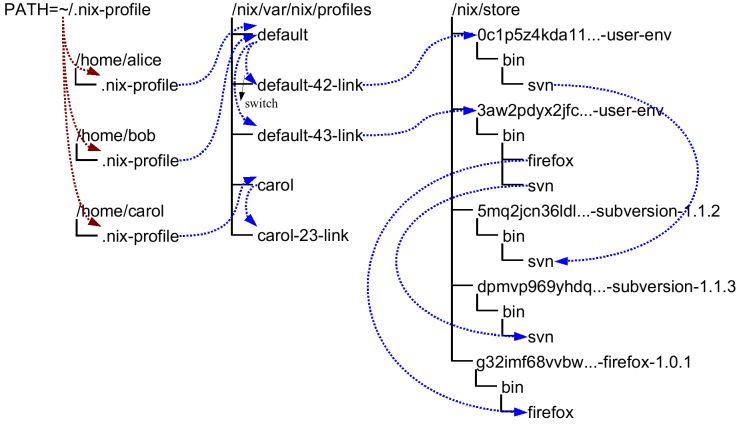
\includegraphics[width=0.85\textwidth]{thesis/graphics/nix-user-environments.png}
  \caption{Directory tree of symlinks in the Nix store (\texttt{/nix/store}) that define the active packages (and their dependencies) of a user environment \cite{Profiles}.}
  \label{fig:nix-user-environments}
\end{figure}

\subsection{Package management}\label{nix-tools-package-management}
Nix provides a collection of Nix expressions, called the \emph{Nix package collection} (Nixpkgs), which is a git repository that contains packages as Nix expressions ranging from build tools like \verb|GCC| and \verb|Glibc| to user applications like Mozilla Firefox. It is possible to write one's own package collection or extend Nixpkgs. To easily stay up to date with new versions of Nixpkgs, we can use the \emph{Nix channel} mechanism \cite{NixPackageManagement}. A nix-channel is a name for the latest ``verified'' commits in Nixpkgs, where ``verified'' is defined on a channel basis. These channels provide binary builds of packages that are cached in the Nix binary cache. One can, for example, add different channels and switch between them on a user-level basis \cite{NixChannels}.

\subsection{User environments and multi-user mode}\label{Nix-multi-user}
In Nix, \emph{user environments} allow atomic updates, atomic rollbacks, and users to have custom configurations. Different users may ``see'' different subsets of the set of all installed applications on the system. This subset is specified in a directory in the user's \verb|PATH| and is called a user environment \cite{NixIntroduction}. 
Nix uses a directory tree of symlinks inside the Nix store depicted in figure \ref{fig:nix-user-environments} to achieve the linking between user environments (\path{/nix/store/0c1p5z4...-user-env}) and the active packages (e.g. \verb|subversion-1.1.2|) they use. The discussion of Nix profiles is out of the scope of this work \cite{Profiles}. %\emph{Generations} outside the store (e.g. \verb|default-42-link|) point to user environments. A new generation is created by each \verb|nix-env| operation (i.e., when installing new packages or changing the profile) and is based on the current one. Generations are grouped into profiles so that users do not interfere with each other \cite{Profiles}.

Nix has a multi-user mode that allows multiple users to safely share a Nix store by ensuring that users cannot arbitrarily run builders that modify the Nix store or database or interfere with other users' builds. User-space limitations achieve this: the Nix store and database are owned by a privileged user, and builders are executed under special user accounts. If an unprivileged user runs a Nix command, then actions that operate on the Nix store are performed by the \emph{Nix daemon} running as the owner of the Nix store \cite{NixMultiUser}. 

\subsection{The \textbf{\texttt{nix-shell}} and \textbf{\texttt{nix-build}} commands}\label{nix-shell&nix-build}
The \verb|nix-shell| command helps reproduce a development environment for a package without building the derivation \cite{NixIntroduction}\cite{NixShell}. Given a Nix expression, the command \verb|nix-shell| constructs an isolated environment with all the inputs needed to run the build script but does not execute the build script as the \verb|nix-build| command. To this end, \verb|nix-shell| builds the dependencies of the expression from the source or downloads them from a binary cache if they are not already in the Nix store. It will then source a setup script that sets all necessary environment variables (e.g., the \verb|PATH|, compiler search path, Nix profile) to their corresponding values. After that, the command starts a shell in which all the environment variables are set.

In short, the \verb|nix-shell| command only sets up a development environment from the expression without building a new derivation. We use the \verb|nix-build| command to build new derivations from an expression. 

\subsection{Nix functions for Docker compatible images}\label{nix-dockertools}
Nix provides a set of functions (\verb|dockerTools|) for creating and manipulating container images. These functions do not need Docker itself for their operations. %The \verb|buildImage| function builds a Docker-compatible tarball containing a single image with multiple layers. 
The \verb|buildLayeredImage| function builds an image with many of the store paths on their own layer, and each is realized as a tarball. The \verb|streamLayeredImage| function streams an uncompressed tarball of an image to \verb|stdout|, which avoids realizing the image into the Nix store, therefore saving on I/O operations and disk/cache space \cite{DockerTools}. Both commands' tarball(s) can be loaded into Docker or pushed to a registry.
\def\Cplusplus{C\raisebox{0.5ex}{\tiny\textbf{++}}}
\chapter{Solution approaches and methodology}\label{methodology}
% describes and justifies the methods to be used in data collection
This chapter describes and justifies approaches and corresponding prototypes that solve the objective of finding feasible approaches to building development environments at runtime based on the lecturer configuration. In addition, we describe how we collect the measurement data for our results. 
\section{Why Nix as image build system}
The current approach of CodeExpert uses Docker as a build system to create container images for different environments and different versions of environments with all required dependencies packaged in the same image. In this section, we will discuss some of the tradeoffs with this approach to justify why we chose Nix as a build system to solve our objective.

Ideally, we want to build reproducible images that contain only the dependencies of the environment and nothing else for repeatable builds to minimize the image size for performance and the attack surface for security. 
\subsection{Issues with the current approach}\label{reproducibility-docker-build}
Apart from the reproducibility issues that arise when building Docker images (see \ref{reproducibility}), the \verb|Dockerfile|'s imperative language cannot always capture the exact dependencies of an image. For example, to configure a \verb|Python| environment, one commonly manages dependencies in multiple ways, such as a base image, copying files into the image, and multiple package managers like apk and pip. Some of these tools are only needed at build-time (e.g., pip, apk) and others at runtime, but both are included in the final image \cite{Wagner2021}. Another thing to notice is that one cannot take two images and combine them. For example, suppose one wants to combine two configurations, a \verb|C++| and a \verb|Python| image. In this case, one has to start with either one of them as a base image and install the dependencies of the other image using \verb|Dockerfile| instructions.

To remedy the problem of capturing the dependencies, one could use multi-stage Dockerfiles. However, this requires optimizing by hand and is just a workaround of proper dependency management \cite{Wagner2021}.
\subsection{Advantages of building images with Nix}
The Nix build system solves the above problems and builds reproducible images that can then be deployed using the advantages of a container ecosystem such as Docker. Nix allows us to install packages in an image without using a base image. Additionally, we can declaratively separate the build from the runtime dependencies so that only the necessary dependencies end up in the final image \cite{Wagner2021}. The result is ``cheap'' images in terms of image size. 

In addition, the properties of Nix introduced in \ref{Nix-theory} enable the following advantages:
\begin{itemize}
  \item Composition of configurations (i.e., base and preset configuration) and environments (e.g., Java and Python)
  \item Efficient caching of dependencies, image layers, and environments for building images at runtime
  \item Simple customization of the configuration (e.g., specific package version) by the lecturer
  \item Developers and lecturers can share package configurations, e.g., in a Nix package repository
\end{itemize}
We introduce what we mean by \emph{base} and \emph{preset configuration} in section \ref{prototype-configuration}.

\section{Solution approaches}
In this section, we introduce the idea of our solution approaches and discuss alternative approaches. We will explain the exact implementations of our approaches in later sections of this chapter. 

\subsection{Approaches for building images at runtime}\label{methodology:approaches-prototypes}
We have developed two feasible approaches that solve our first objective. Each approach's goal is to create an isolated environment at runtime where all dependencies are installed, given an environment configuration by the lecturer. Our approaches should integrate into the existing architecture of CodeExpert. Thus our approaches build environments similar in purpose and function to the cxEnvironment containers (see \ref{CodeExpert}), which has the following implications for the design of our prototypes.
%Unlike the lecturers who configure the environment first, we assume that the students run this environment many times and need a quick startup time. This assumption means that our prototypes prioritize the performance of subsequent environment creations among multiple simultaneous students with the same configuration over the performance of the first-time build. 

Apart from prioritizing the subsequent-startup time over the first-build time, our design considered that environments only execute a single job and are removed afterward. Ultimately, the images corresponding to the environments need to be pushed to a central registry where they are stored.

\paragraph{Build image at runtime (BIAR)}
BIAR builds a new image at runtime for every new configuration. The essential idea is to have ``builder'' containers with Nix installed that build a new image based on the lecturer configuration and then push the resulting image to a registry. Afterward, we can pull the image from the registry and start an environment with it. An environment does not need Nix installed, as all packages are added to the image at build time. Any number of builder containers can run in parallel and operate on a shared Nix store. 
\paragraph{Nix-shell at runtime (NSAR)}
Unlike BIAR, NSAR does not build a new \emph{image} at runtime. Instead it creates a new environment using the \verb|nix-shell| command with all packages in the configuration installed (see \ref{nix-shell&nix-build}). The \verb|nix-shell| is run inside a container that needs to be started first and has Nix installed. NSAR creates all these containers from a single image, and their Nix installation shares the same Nix store.
\subsection{Alternative approaches}
We considered using a tool of the Nix ecosystem called Nixery as a different approach somewhat similar to BIAR for solving our problem. Nixery provides ad-hoc containers, including any packages from a package repository, such as Nixpkgs (see \ref{nix-tools-package-management}). The images are built by Nix using a particular layering algorithm, optimizing cache efficiency. Nixery has a custom caching algorithm for layers that extends the \verb|buildLayeredImage| function of Nix \cite{Nixery}. 

This approach proved too inflexible, as one can only specify an environment by providing a list of packages by name, thereby losing the flexibility of a Nix expression \cite{Nixery}. Specifying packages by name would not allow lecturers to easily use custom packages with specific versions or environments with an interpreted language. Therefore we have dropped this approach from further consideration. 

\section{Configuration}\label{prototype-configuration}
Both approaches share the same configuration scheme. There are two groups of configurations: \emph{base} and \emph{preset}. The base group, denoted by $C_{base}$, contains a single configuration file that specifies the dependencies used by every environment. An example configuration file that specifies the GNU Core Utilities and Bash is shown in \nameref{base.nix}. 
\begin{lstlisting}[caption={base.nix}, title={base.nix}, label={base.nix}]
{ pkgs }:
{
  inputs = with pkgs; [ 
    coreutils-full 
    bashInteractive 
  ];
}
\end{lstlisting}
The preset group, denoted by $C_{preset}$, contains predefined configurations (e.g., \verb|Python|, \verb|C++|) from which the lecturer can choose one configuration and fully customize it -- potentially removing all packages. An example preset configuration for \verb|C| is shown in \nameref{preset.nix}. 
\begin{lstlisting}[caption={preset.nix}, title={preset.nix}, label={preset.nix}]
{ pkgs }:
{ inputs = with pkgs; [ gcc gdb ]; }
\end{lstlisting}
Sometimes we talk about the entire package set that is available in an environment, called $C_{result}$, that is the union of $C_{base}$ and $C_{preset}$. To continue our example, the $C_{result}$ of \nameref{base.nix} and \nameref{preset.nix} is the union of the package sets and shown in \nameref{result.nix}.
\begin{lstlisting}[caption={result.nix}, title={result.nix}, label={result.nix}]
{ pkgs }:
{
  inputs = with pkgs; [
    coreutils-full
    bashInteractive
    gcc
    gdb
  ];
}
\end{lstlisting}
All configuration files, in particular the configuration that the lecturer specifies, have a specific interface that restricts the definition of dependencies to a list of inputs -- denoted by the \verb|inputs| attribute. The interface establishes that the build process can correctly read (and eventually join) the dependencies from the configuration files. Furthermore, in the case of a file in $C_{preset}$, this interface has two additional purposes. First, it removes syntax -- simplifying the expression the lecturer needs to write. Second, it restricts the lecturer from using arbitrary Nix expressions as a configuration. The interface may need additional attributes to allow the lecturer to specify, for example, environment variables such that the interpreter finds all libraries.

We split the configuration to show how easy it is to merge different configurations with Nix and better separate and combine different configurations for our measurement process. The two configuration groups could be unified from the beginning into a single file that the lecturer can edit. This file would make all environment dependencies directly transparent to the lecturer.
\section{Prototype: Build Images At Runtime}
This section describes the prototype of the Build Images At Runtime (BIAR) approach and its components.
\subsection{Components}\label{BIAR-components}
The essential component of our prototype is the \emph{builder container} (see fig. \ref{fig:BIAR-execution-flow}). This container is started every time a new image needs to be built from a configuration. It has Nix installed and has a persistent and shared Nix store mounted as a volume into the container. Using shared persistent storage for the content-addressable Nix store makes it possible to have multiple builder containers perform parallel builds using the store as a shared build cache. 

The container takes the configuration as input and uses \verb|nix-build| to build a new layered image. Depending on the build function used \\((1) \verb|streamLayeredImage| or (2) \verb|buildLayeredImage|), the output of the build is then pushed to a registry by either (1) streaming its compressed layers to the registry or (2) copying the compressed tarball from the Nix store to the registry (see \ref{nix-dockertools}). We build a layered image since this allows Nix to optimize the caching of the layers. Efficient caching is essential for this approach as we want to utilize the heuristic that configurations often share most packages to build new images as fast as possible at runtime. 

Our prototype includes a ``BIAR-data-container'' container that creates a volume with the shared Nix store inside and can be used to perform management operations, e.g., running the garbage collector on the store's data.
\subsection{Execution flow}\label{BIAR-execution-flow}
The execution flow differs depending on the first or subsequent times the image is built from the same configuration. We assume in the following that a builder container has been started with an arbitrary but fixed $C_{result}$ as input (see fig. \ref{fig:BIAR-execution-flow}).

\begin{figure}
   \centering
   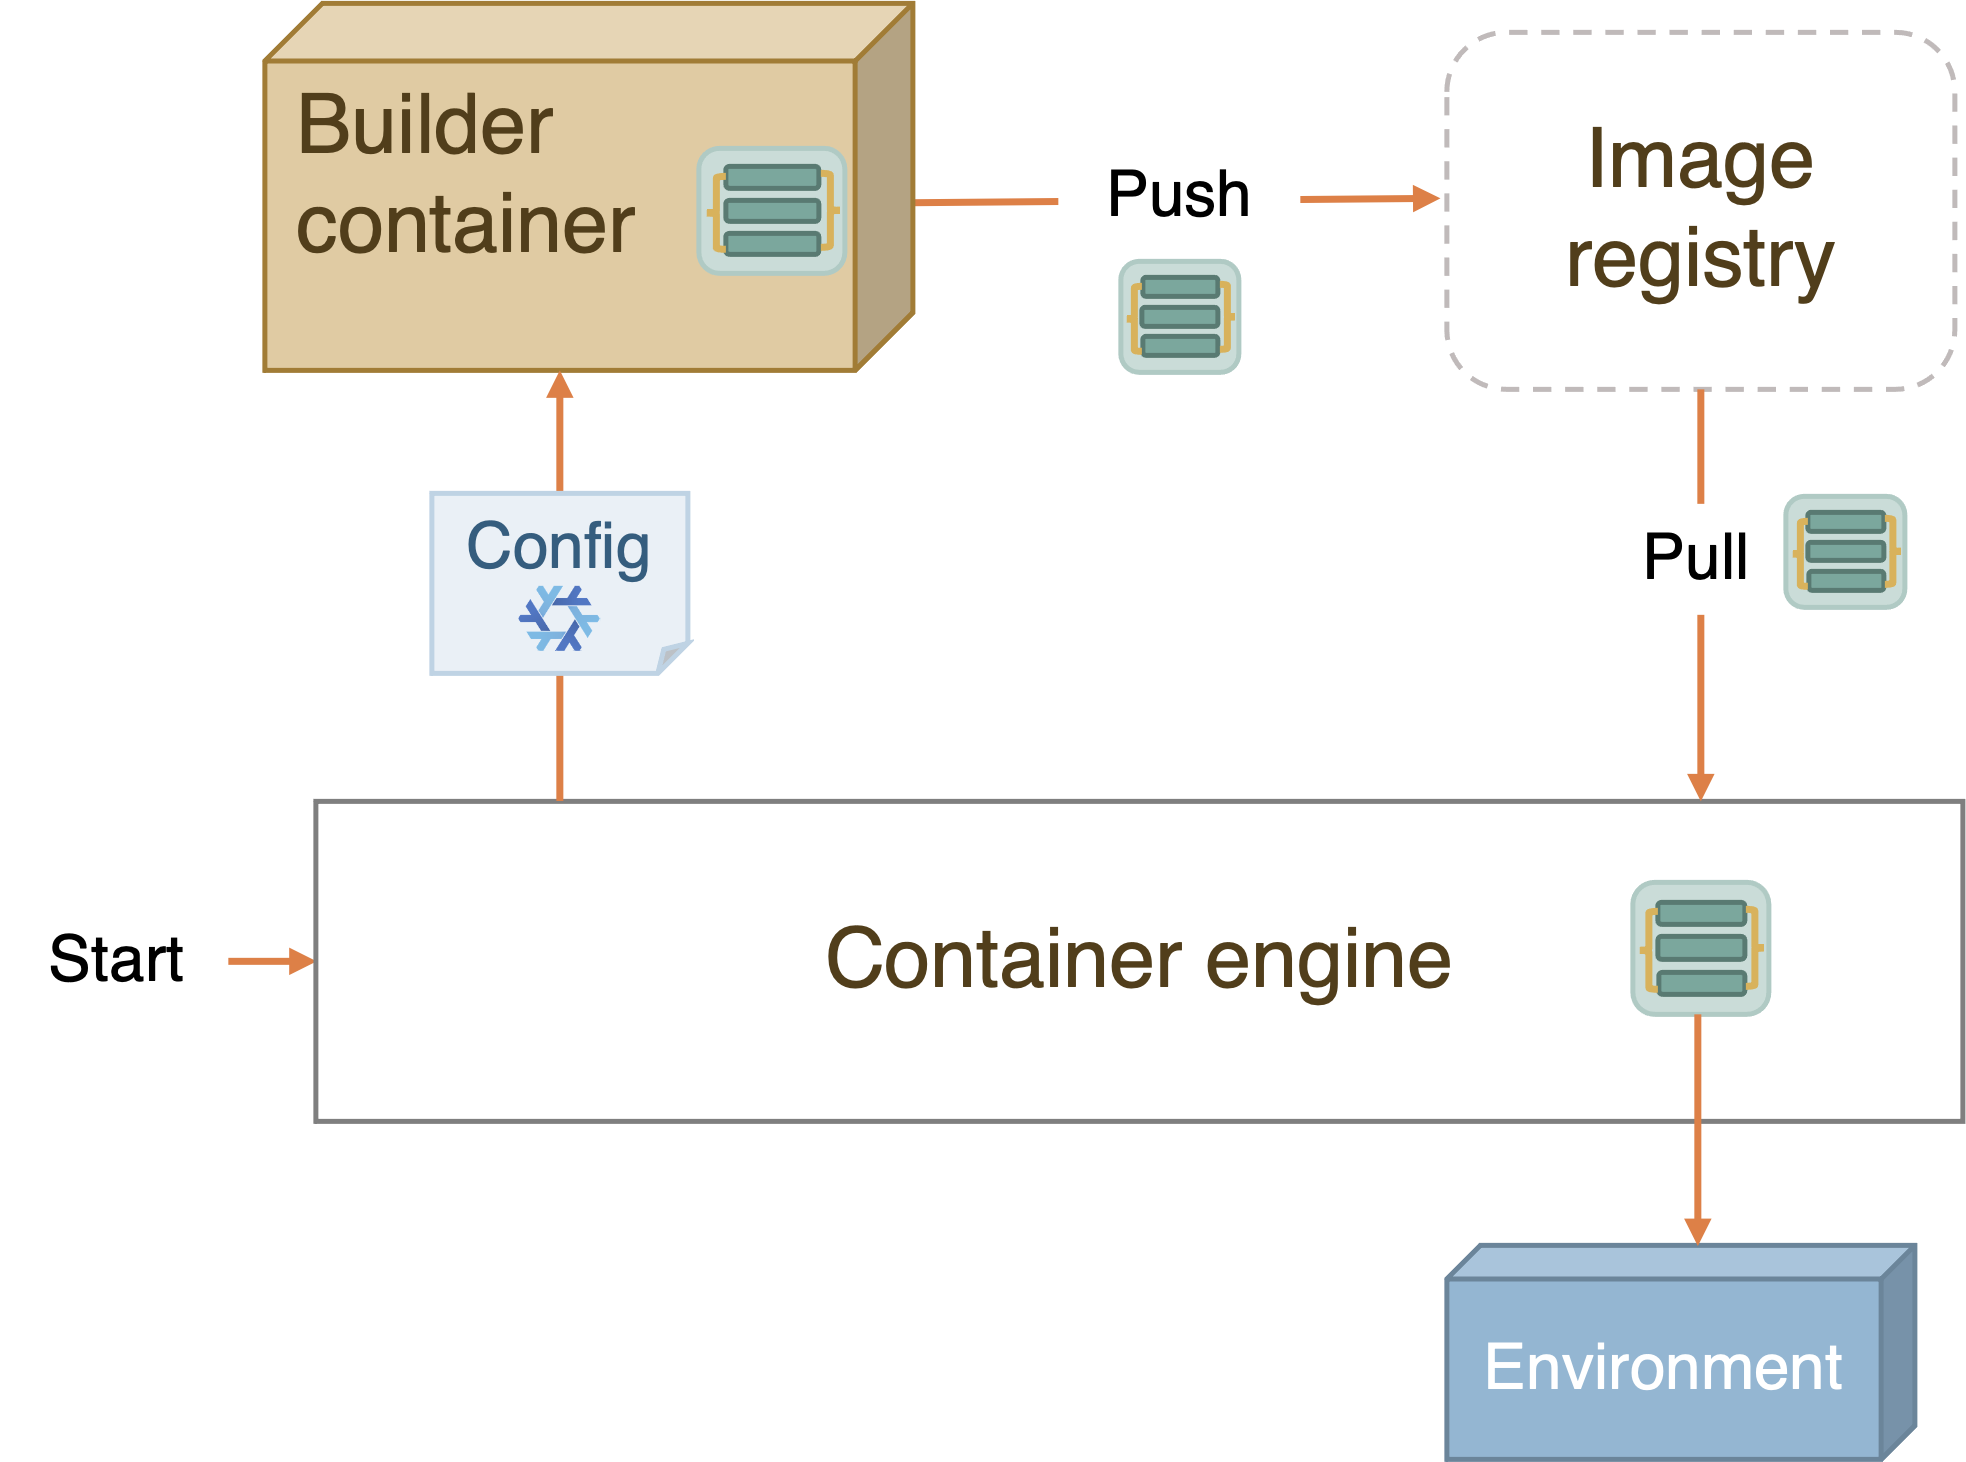
\includegraphics[width=0.6\textwidth]{thesis/graphics/BIAR-execution-flow.png}
   \caption{Build images at runtime approach: components and execution flow} 
   \label{fig:BIAR-execution-flow}
\end{figure}

In the case of the first-time build, the Nix store is empty, and Nix must either download the needed derivations from a binary cache or build them from source code and write them to the store. Once all derivations are available, Nix builds a layered image and pushes the layers to the image registry. The container engine on the host then pulls the image from the registry and starts a container from it, where the environment is ready. The host container engine knows which image to pull and start using the mechanism explained in (\ref{identify-images-with-configuration}). 

In the case of subsequent-time builds, Nix can omit to rebuild the derivations and layers and use the layers cached in the Nix store. We explain how Nix caches layers efficiently in section \ref{efficient-caching-of-layers}. This caching allows subsequent builds to be almost instant. However, we cannot cache pushing the image to the registry with our implementation, whether it is the first or subsequent push of the same image. The key idea to make subsequent builds quick is to notice that subsequent-time builds with the same $C_{result}$ imply that a copy of the image is already cached locally on the host container engine. Thus we can omit the build and the push step and start an environment from the cached image. This execution flow requires that the container engine must determine if an image has already been built with a given $C_{result}$ (see \ref{identify-images-with-configuration}). 

Another thing to notice is that if the lecturer changes his configuration only by a ``small'' amount (i.e., adds/removes a few packages) in a subsequent build, then we can expect that most derivations and layers are cached in the store from a previous build. We expect this since many packages share the same base dependencies \cite{Christensen2018}. Since Nix can cache layers and derivations efficiently, the build of a small configuration change will be faster than a first-time build.

\subsection{Identify image from configuration}\label{identify-images-with-configuration}
Generally, a container image can be identified by its name and tag. We used the following convention in our prototype: the image name is the hash value of the base configuration's content that does not often change, whereas the image tag is the hash value of the lecturer configuration file. 

Since we build a new image for every configuration change, we need to be able to identify an image from its configuration uniquely. This means we need an injective function \(f\colon X\to \mathbb{H}\) with domain $X={(f_1, f_2,\dots)}$ of configuration files $f_i$. However, we use the \textsc{MD5} hashing algorithm as our function $f$, which is not injective and has collision vulnerabilities \cite{Stevens2012}. Nevertheless, we use this algorithm because performance is critical, random collisions are rare, and we do not need to worry about collision attacks from lecturers (explained in \ref{discussion:security}). Performance matters, as we must compute the function $F$ before starting any environment.

\iffalse
To compute a unique hash value of multiple files, we would need an injective function \(F\colon X\to y\) that maps from the domain $X={(f_1, f_2,\dots,f_n)}$ of $n$ files $f_i$ and to a unique output $y$. We use the following definition of $F$: 
\begin{gather*}
  F(X) = hash(hash(f_1) + hash(f_2) + \dots + hash(f_n)), \\
  \text{where}~+ \text{means concatenation and}~hash \text{ is the chosen hash function.} 
\end{gather*}
Since the composition of injective functions is injective we need $hash$ and $+$ to be injective. Since every hash value has a fixed length, ambiguity cannot arise from the concatenation ($+$) operation. However, we use the MD5 algorithm as our $hash$ function which is not injective and has collision vulnerabilities \cite{Stevens2012}. Thus our function $F$ is not injective. 

We still use the MD5 algorithm because performance is critical, random collisions are rare, and we do not need to worry about collision attacks. Performance matters, as we must compute the function $F$ before starting any environment.
\fi

\subsection{Efficient caching of layers}\label{efficient-caching-of-layers}
The efficient caching of layers is essential for this approach as changes to configurations will likely result in only very few changes of dependencies that need to be built or rebuilt. If we can cache the building of as many unchanged dependencies as possible, it would result in a faster build time and less disk usage.

It is not easy to make the caching of layers efficient as most package managers mutate global directories (see \ref{Nix-theory}), resulting in having to take a diff of the whole filesystem (see \ref{images-and-layers}). This is similar when using Docker as the image build system, where Docker only sees the diff of the whole filesystem and cannot determine the exact file changes resulting from, e.g., package manager operations. Therefore it cannot know that installing package ``foo'' has nothing to do with the package ``bar'' and that the changes are separately cachable. The caching behavior can be improved by manual optimization in a \verb|Dockerfile|, for example, adding one's files after installing packages or installing all packages in a single instruction \cite{Christensen2018}.

Nix caches dependencies and improves sharing between images by having layers equal to a store path representing a dependency. Nix can automate the cache optimization because it restricts package builds to writing to specific places on disk (namely the \$out directory of the Nix store). Other reasons are that Nix knows all dependencies from the dependency graph and stores build outputs in immutable files and unique paths. Since the Docker image specification limits the number of layers, Nix combines the dependencies that are less likely to be a cache hit into one layer. Dependencies that are shared the most by multiple packages are more likely to be a cache hit. Thus Nix makes separate layers for these ``popular'' dependencies. Using more layers increases the number of layers that could be shared between images. The shared layers are likely not affected by a configuration change. This avoids rebuilding and increases the caching efficiency \cite{Christensen2018}. Both the \verb|buildLayeredImage| and \verb|streamLayeredImage| (see \ref{nix-dockertools}) functions use the optimized layer caching algorithm. 
\section{Prototype: Nix-Shell At Runtime}
This section describes the prototype of the Nix-Shell At Runtime (NSAR) approach and its components.
\subsection{Components}
Our implementation of the NSAR approach has \emph{one image}, built with Nix. It is based on the \verb|nixos/nix| image from the Docker Hub, which has Nix and some runtime dependencies required by Nix installed. In this base image (see fig. \ref{fig:NSAR-execution-flow}), we install the dependencies of $C_{base}$ at build time, as they are the same for every container. 

Our prototype has a container called ``NSAR-data-container'' that creates two volumes similar in purpose to the BIAR-data-container. One for the persistent shared Nix store and the other for the persistent \verb|nix-shell| cache explained in \ref{caching-nix-shell}. Both caches are pictorially depicted as one shared cache in fig. \ref{fig:NSAR-execution-flow}.

\begin{figure}[h!]
   \centering
   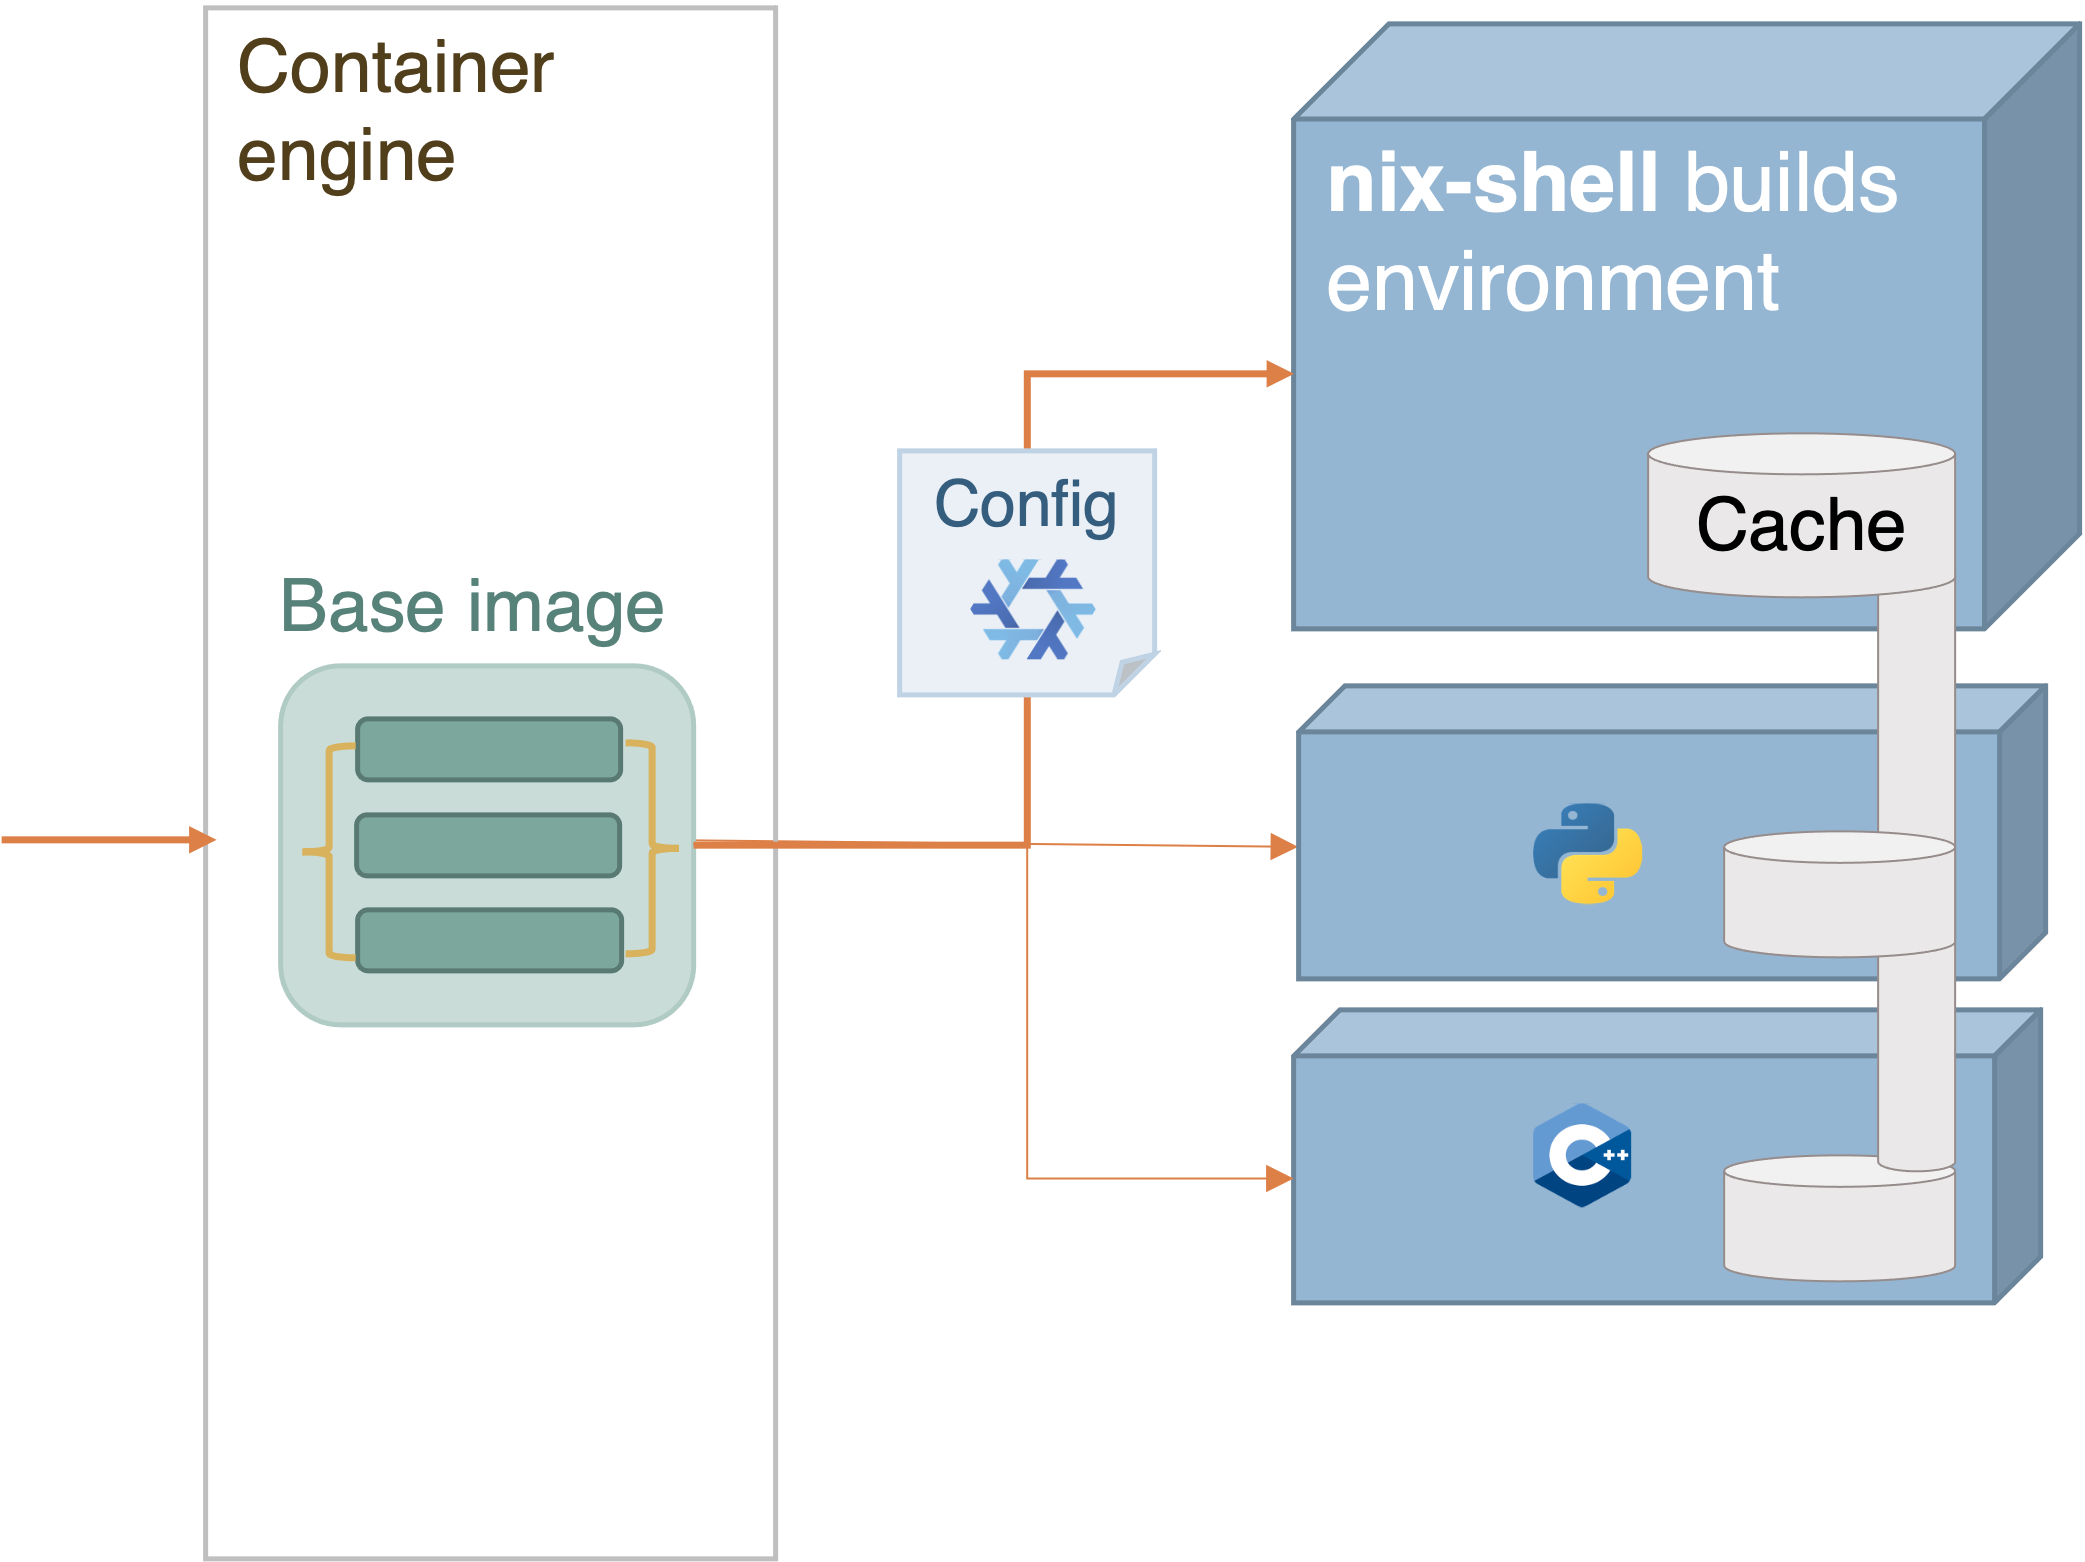
\includegraphics[width=0.6\textwidth]{thesis/graphics/NSAR-execution-flow.png}
   \caption{Nix-shell at runtime approach: components and execution flow} 
   \label{fig:NSAR-execution-flow}
\end{figure}

\subsection{Execution flow}
Unlike BIAR, NSAR does not build a new image at runtime; instead, this approach creates an environment at runtime inside a prebuilt container. We assume that a container was started from the base image and has an arbitrary but fixed lecturer configuration from $C_{preset}$ as input (see fig. \ref{fig:NSAR-execution-flow}).

The execution flow differs depending on the first or subsequent times \verb|nix-shell| creates the environment from the same configuration. In the case of the first-time build, the Nix store is empty. The empty store results in the \verb|nix-shell| having to download the derivations from a binary cache or build them from source code. In the other case, we can assume that the Nix store contains all derivations from previous builds with the same configuration, and the \verb|nix-shell| will skip the downloading or building step.

The execution flow continues with the \verb|nix-shell| setting up a development environment, as described in greater detail in \ref{nix-shell&nix-build} from the lecturer configuration. In particular, our prototype calls the \verb|nix-shell| command with a proxy file (\verb|nixproxy.nix|) as input that defines a new environment with the given configuration's dependencies. 

The purpose of this proxy file is twofold: to check the input interface of the configuration files and fix, among others, the version of the package collection (e.g., of Nixpkgs). Another thing to notice is that the interface to the lecturer in the configuration files of $C_{preset}$ can be extended for this approach with a \verb|shellHook|. The \verb|shellHook| is run after the setup file has been sourced (see \ref{nix-shell&nix-build}). This hook performs initialization specific to the \verb|nix-shell| and allows the lecturer to define bash statements that will be executed when starting the shell \cite{NixShell}. This shellHook is very useful, for example, to export environment variables, and create hidden output files.

Recall that the Nix store is persistent and shared across the environments as a volume. This sharing is necessary so that only the first student will experience the first-time environment build discussed above. All other students will experience the ``subsequent build time'' case as the Nix store acts as a build cache, provided they use the same configuration. This mechanism ensures that subsequent builds are quick and that only the first environment build is slow, as our specification requires.
\subsection{Caching the \textbf{\texttt{nix-shell}} execution}\label{caching-nix-shell} 
To make subsequent build times of an environment faster, we would like to skip the last remaining step of the \verb|nix-shell| execution: the evaluation of the setup file (see \ref{nix-shell&nix-build}). It is possible to omit this step by caching its result: the exported variables and reuse them on subsequent runs. This caching can be accomplished with different tools in the Nix ecosystem, such as \verb|direnv| with \verb|Nix-direnv| or Nix flakes. 

In this prototype, we use the \verb|cached-nix-shell| tool \cite{CachedNixShell}, as it traces all configuration files used during evaluation and performs cache invalidation if any used files change. This tool stores the inputs and outputs of the derivation and the traces (configurations) of the nix-shell invocation as content-addressable files inside the \verb|~/.cache/cached-nix-shell| directory.

To persist this cache after the container lifecycle, we store the cache of this tool as a volume. The persistence is necessary since the speedups from the subsequent use of the same configuration need to remain over multiple container startups (see \ref{methodology:approaches-prototypes}). 
\subsection{Seeded Nix store}\label{seeded-nix-store}
As an additional consideration, the prototype allows for using a seeded store, which means we prepopulate the store with derivations (with the \verb|nix-env| command; introduced in \ref{nix-tools-package-management}). A store with the most popular derivations installed can improve the first-time build performance of an environment as Nix can skip downloading derivations from the binary cache if they are already available in the Nix store. 

%\section{Test environments}\label{test-environments}
%We evaluate our prototypes with \verb|Python| and a \verb|C|/\verb|C++| environment. The following sections will explain their differences and similarities such that we can evaluate if our prototypes perform differently in one or the other environment. The packages used for the benchmarks included in each environment are listed in \ref{appendix:bench-envs-packages}.
%\subsection{Python}
%\verb|Python| is a high-level programming language implemented in \verb|C|. It supports multiple programming paradigms such as functional and object-oriented and is an \emph{interpreted language}. The \verb|Python| ecosystem has two commonly used interpreters, \verb|PyPy| and \verb|CPython|. \verb|CPython| interprets the source code by first converting it into byte code and then compiling it into machine code at run time. On the other hand, PyPy directly compiles the source code to machine code at run time with its JIT (Just in Time) Compiler. \verb|PyPy| is usually faster than \verb|CPython| since it ``skips'' the conversion to byte code. We use the \verb|CPython| interpreter in our prototype since it is the same interpreter used by the current CodeExpert \verb|Python| environments. 

%\verb|Python| is a dynamically typed language implying the interpreter has to check the variable type at runtime, slowing the execution time and leading to more memory allocation. \verb|Python| uses automatic memory management and garbage collection, which increases the program's runtime, as it takes time to identify what memory to free during which the interpreter cannot run. 
%\subsection{\Cplusplus}
%\verb|C++| is an Object-Oriented Programming language. It is statically typed; Every variable is stored with its data type, which removes the need to check the type conversions at runtime and results in faster execution. \verb|C++| is a \emph{compiled language}, unlike \verb|Python|, which means that the source code is compiled into machine code by the compiler before it can be executed. Thus, once compiled, \verb|C++| code is faster than \verb|Python|. Furthermore, \verb|C++| does not use a garbage collection, improving the performance compared to \verb|Python|.

\section{Methods for data collection}\label{methods-for-data-collection}
To evaluate our prototypes, we performed measurements using a virtual machine running on Ubuntu 20.04.4 LTS. After two ``warmup'' iterations, we measured each command for ten repetitions. The warmup phase ensures that we measure the steady-state performance of our machine as there is an initial overhead from empty caches and TLBs, causing costly misses for memory accesses.

\subsection{Statistical test}
We computed the pairwise significance between the means of each benchmark data sample to compare our results based on a statistical test. We assume independence between two samples since they are measured independently. If the variance of both samples is the same, we used a two-sample t-test; otherwise, we used Welch’s t-test, which does not assume equal variance. We followed a common rule of thumb to decide whether the variances are similar (the formula is explained in \ref{appendix:statistical-test}). We use the p-value to assess the statistical significance with a level of 0.05.
\subsection{Software}
We ran the benchmarks with a custom bash script that uses the GNU Time command to measure the process time statistics. We used our results' \emph{Real time} part of the time commands output. This is the wall clock time -- the time from start to finish of the call and is the actual elapsed time of the process, including time spent blocked, e.g., waiting for I/O and time slices used by other processes.
\subsection{Hardware}
The remote virtual machine's hardware comprises two virtual CPUs (Intel Family 6 Model 63 Stepping 2) running at 2GHz with 2GB of memory. A virtual CPU corresponds to a single hyperthread on a processor core. The VM system includes a 60GB SSD disk, and the memory throughput could not be determined as the VM service does not support this information. 

\subsection{Test environments}\label{test-environments}
We evaluate our prototypes in two different test environments to verify if our prototypes perform differently in one or the other environment. The first is a \verb|Python| environment, an example of an interpreted language. The second is a \verb|C|/\verb|C++| environment as an example of a compiled language. The packages used for the benchmarks included in each environment are listed in \ref{appendix:bench-envs-packages}.
\chapter{Results}\label{results}
We evaluate our prototypes using four evaluation criteria: \emph{performance}, \emph{user experience}, \emph{developer experience,} and \emph{security}. Each section in this chapter is dedicated to one criterion.
\section{Performance}\label{results:performance}
We assess the performance of our prototypes for the two test environments, \verb|C++| and \verb|Python|. We first handle the results concerning the implementation details of each prototype. Afterward, we compare them with each other and to the current approach of CodeExpert on the two build cases: first-time and subsequent-time build. We refer in the following to a ``full Nix store'' if we benchmark a subsequent-time build where Nix can use the cached results in the Nix store of the first-time build. An ``empty Nix store'' contains no pre-downloaded binaries of packages.

We made the measurement process of all approaches as comparable as possible by deciding what execution flow resembles the corresponding build case in the best way for each approach. This decision is made separately due to the different implementations and is explained at the beginning of sections \ref{first-time-build} and \ref{subsequent-time-build}. In every benchmark that measures an environment's startup time, the time needed to stop and remove the container is also included in the measured real-time. Therefore the time until the environment is ready to execute the user's code is faster than what was measured.

\subsection{BIAR: approach specific}\label{biar-approach-specific}
For the BIAR approach, we want to determine which strategy (layered or streamed) is better to build images in the builder container and push them to the registry (see \ref{BIAR-components}). We use a registry running inside another container on the same host to simulate the current image registry execution flow of CodeExpert (see \ref{CX-configuration}). We only show the figures of the \verb|Python| environment, as the differences between the strategies are similar for the \verb|C++| environment.

\begin{figure}[h!]
  \centering
  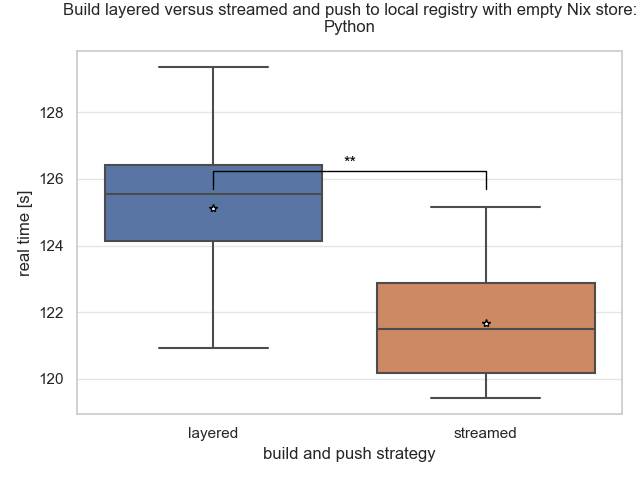
\includegraphics[width=0.71\textwidth]{thesis/graphics/biar-plots/build_layered_versus_streamed_and_push_to_local_registry_with_empty_nix_store:_python.png}
  \caption{Comparing the build and push strategies streamed and layered using an \emph{empty} Nix store. Remarks: * = a higher number of stars(*) indicates a greater statistically significant difference}
  \label{fig:biar-layered-vs-streamed-full-store-python}
\end{figure}

When the Nix store is empty, we observe that streaming is significantly faster for both \verb|Python| and \verb|C++| environments than the layered strategy (see fig. \ref{fig:biar-layered-vs-streamed-empty-store-python}. However, when we used a full cache (Nix store), there was no significant difference between the strategies, as shown in figure \ref{fig:biar-layered-vs-streamed-full-store-python}.

\begin{figure}[h!]
    \centering
  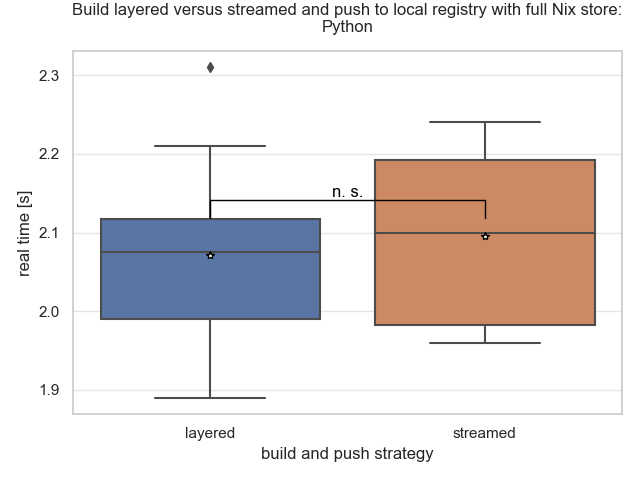
\includegraphics[width=0.71\textwidth]{thesis/graphics/biar-plots/build_layered_versus_streamed_and_push_to_local_registry_with_full_nix_store:_python.png}
  \caption{Comparing the build and push strategies streamed and layered using a \emph{full} Nix store.
  Remarks: n.s. = statistically nonsignificant difference}
  \label{fig:biar-layered-vs-streamed-empty-store-python}
\end{figure}

The measured times are almost identical in the full Nix store case since both strategies use the store as a cache and skip building the image. In this case, the build time is dominated by the time (approx. 2s) it takes to push the layers to the registry. This push time means that even with caching the image built in the builder container, the current prototype's build time is still bounded by the push time. This influenced the prototype's design to skip the push step in \ref{BIAR-execution-flow}. When the cache is empty, the build time is dominated by the building of the image, which takes approx. 120s, and not by the push time, which is only around 2s.

\subsection{NSAR approach specific}
To determine the best internal implementation of the NSAR approach, we show our results of caching the nix-shell and using a seeded Nix store in the following paragraphs.

\paragraph{Caching nix-shell}
We want to test the performance of our idea of caching the nix-shell (see \ref{caching-nix-shell}) with benchmarks. We restrict ourselves to the \verb|C++| environment, as the results are similar to the \verb|Python| environment.

First, we assess the case where the Nix store is full (see fig. \ref{fig:nsar-cached-vs-uncached-full-store-python}), where the environment build-time with the cached nix-shell is almost three times faster than the uncached one. This is because the cached nix-shell can use the cached environment variables and skip the evaluation of the input files. Thus it is faster than the uncached nix-shell. When we assess first-time builds, where the Nix store is initially empty, we observe almost the opposite -- the cached nix-shell is slower than the uncached nix-shell by approx. 20\% (see fig. \ref{fig:nsar-cached-vs-uncached-empty-store-python}). This is because the cache has to be initialized and updated by the cached nix-shell, which incurs some overhead.

\begin{figure}[h!]
    \centering
    \begin{subfigure}{\textwidth}
        \centering
      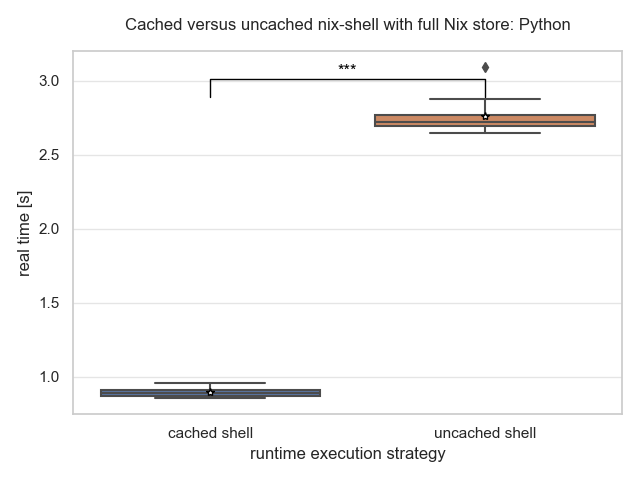
\includegraphics[width=0.75\textwidth]{thesis/graphics/nsar-plots/cached_versus_uncached_nix-shell_with_full_nix_store:_python.png}
      \caption{Comparison using a full Nix store}
      \label{fig:nsar-cached-vs-uncached-full-store-python}
    \end{subfigure}
    \begin{subfigure}{\textwidth}
      \centering
      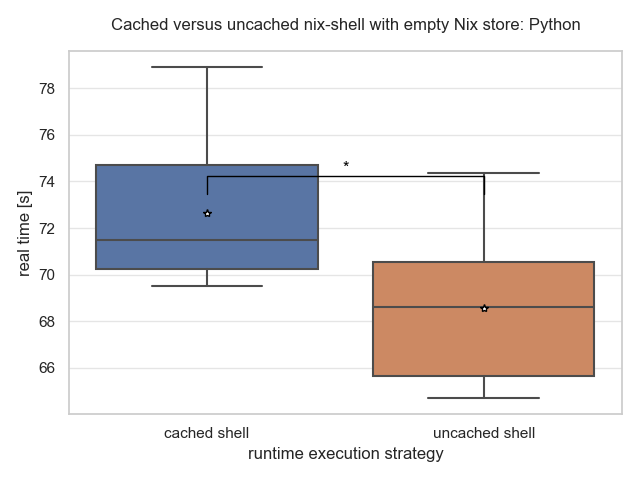
\includegraphics[width=0.75\textwidth]{thesis/graphics/nsar-plots/cached_versus_uncached_nix-shell_with_empty_nix_store:_python.png}
      \caption{Comparison using an empty Nix store}
      \label{fig:nsar-cached-vs-uncached-empty-store-python}
    \end{subfigure} 
    \caption{The ``full store'' is a measurement of a subsequent-time build that uses the cached results of a first-time build with the same configuration. The Nix store is empty for the first-time build. We show the Python environment results. Remarks: cached shell = cached nix-shell (see \ref{caching-nix-shell}), uncached shell = standard nix-shell (see \ref{nix-shell&nix-build}), * = a higher number of stars(*) indicates a greater statistically significant difference.}
    \label{fig:nsar-cached-vs-uncached}
\end{figure}

\paragraph{Seeded store}\label{results-seeded-nix-store}
To determine whether the idea of using a seeded store (see \ref{seeded-nix-store}) improves the performance, we compared it to an empty store and a full store. We prebuild the Nix store with the packages from the $C_{base}$ file as these packages are known at build time and do not depend on the lecturer’s modification. Additionally, we prebuild the Nix store with the packages specified in \ref{appendix:bench-envs-packages} and use a configuration with some additional packages for benchmarking the build time. These additional packages should simulate a configuration modification, where some popular packages are in the seeded store, and the lecturer wants to install some more that are not yet available. We use a cached nix-shell for both comparisons and restrict ourselves to show the \verb|C++| environment here.

\begin{figure}
    \centering
    \begin{subfigure}{\textwidth}
        \centering
      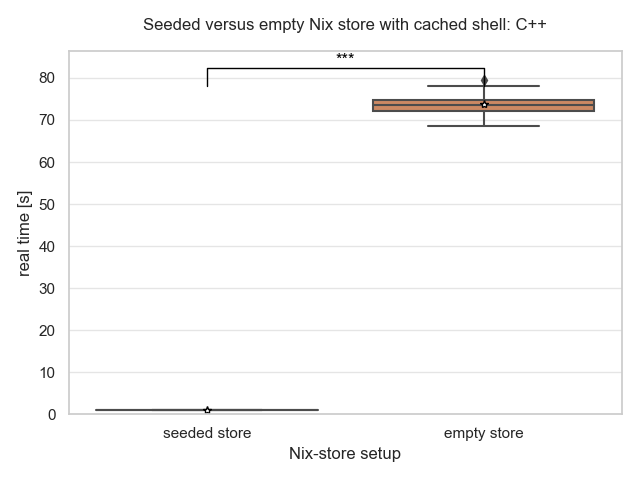
\includegraphics[width=0.75\textwidth]{thesis/graphics/nsar-plots/seeded_versus_empty_nix_store_with_cached_shell:_c++.png}
      \caption{}
      \label{fig:nsar-seeded-vs-empty-store-cpp}
    \end{subfigure}
    \begin{subfigure}{\textwidth}
    \centering
      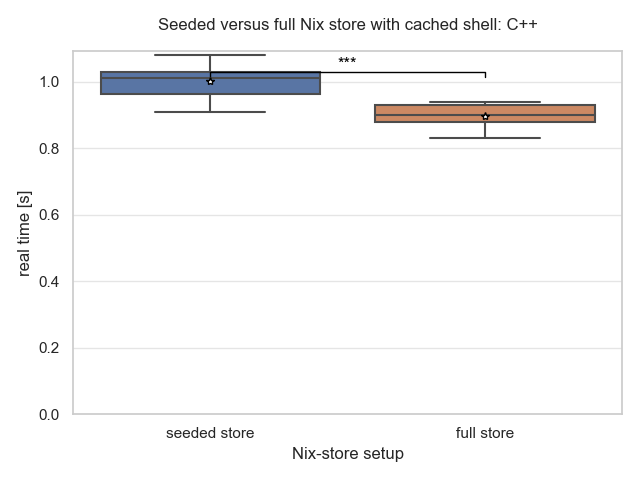
\includegraphics[width=0.75\textwidth]{thesis/graphics/nsar-plots/seeded_versus_full_nix_store_with_cached_shell:_c++.png}
      \caption{}
      \label{fig:nsar-seeded-vs-full-store-cpp}
    \end{subfigure} 
    \caption{The ``seeded store'' has a subset of the packages used to build the measured build time preinstalled. The ``full store'' is a measurement of a subsequent-time build that uses the cached results of a first-time build with the same configuration. We show the \texttt{C++} environment results. Remarks: * = a higher number of stars(*) indicates a greater statistically significant difference.}
    \label{fig:nsar-seeded}
\end{figure}

When comparing the build time of an empty store with that of a seeded store, we can observe that the latter brings an order of magnitude (50x) improvement in performance (see fig. \ref{fig:nsar-seeded-vs-empty-store-cpp}). 

By inspecting figure \ref{fig:nsar-seeded-vs-full-store-cpp}, we note that there is small (approx. 100ms) but signifficant difference when using a seeded store versus a full store. Interestingly when comparing both environments (fig. \ref{fig:nsar-seeded-vs-full-store-cpp} and fig. \ref{appendix:seeded-nix-store-python}) we observe that the \verb|Python| version has a smaller statistical difference (two stars) than the \verb|C++| one (three stars) even though we add 1 \verb|Python| package and 5 OS-packages to the \verb|Python| configuration compared to only 1 additional package in case of the \verb|C++| configuration change (see \ref{appendix:bench-envs-packages}). 


\subsection{First-time build}\label{first-time-build}
The first-time build performance -- starting from the new configuration until the container environment is “ready” -- corresponds to the case where all build-caches are empty. This case happens, for example, when the configuration $C_{result}$ specified by the lecturer is such that no previously cached outputs can be used. We made the measurement process of the approaches as comparable as possible by deciding what execution flow resembles the first-time build in the best way for each approach. This decision is made separately due to the different implementations. We explain how we measured the build time for each approach next.

In the BIAR prototype, we assume that the builder container image is available and the shared Nix store of the builder container is empty. We measure the following steps: start the builder container, then build and push the layered image built from $C_{result}$ as a stream to the registry. Then pull the built image from the registry, and start an environment container from it. 

We measure the build time of the NSAR by assuming that the shared Nix store of the environment container is empty and the minimal base image is cached locally on the container engine host. We measure the following step: start the environment container with the configuration and project files bind-mounted into the container and run the cached nix-shell to build the environment with the packages available. 

In the current CodeExpert approach, the cxEnvrionment image extends the base image \verb|base-rhel8|. We assume this base image is already built, as the lecturer configuration change does not influence it. We measure the following steps: build the cxEnvrionment image, then pull this image from the registry, and start a container from it. We use the \verb|Python-3_8| and \verb|GCC| images and compare them to our \verb|Python| and \verb|C++| environments, respectively. We did not measure the time it takes to push the image to the registry for this approach.

We can start an environment without network access for BIAR and the current approach, unlike the NSAR environments.

\paragraph{Prototypes compared with each other}
Depending on the environment, the NSAR prototype is two to four times faster than the BIAR approach (see figure \ref{fig:nsar-biar-first-time-build-python}). This considerable difference is due to the additional work BIAR does. Both prototypes need to download almost the same packages from the binary cache. However, the BIAR approach must additionally build an image, then push it to and pull it from the registry. Since the significant difference is large for both environments, we only show the \verb|C++| environment’s figure here. 
\begin{figure}
  \centering
  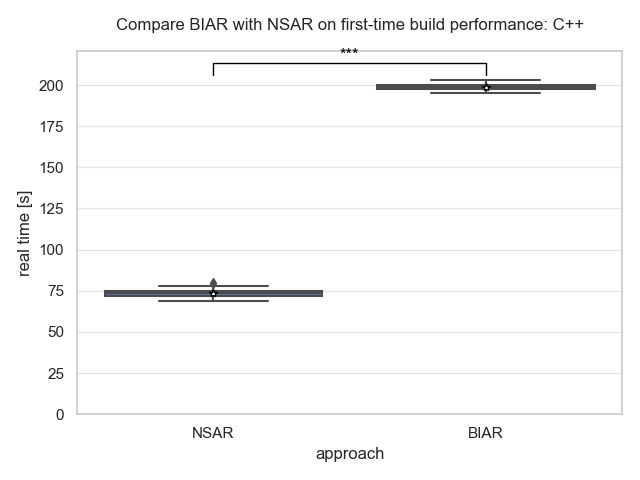
\includegraphics[width=0.75\textwidth]{thesis/graphics/compare-plots/compare_biar_with_nsar_on_first-time_build_performance:_c++.png}
  \caption{Remarks: \texttt{C++} = \texttt{C++} environment, NSAR = nix-shell at runtime, BIAR = build image at runtime, * = a higher number of stars(*) indicates a greater statistically significant difference.}
  \label{fig:nsar-biar-first-time-build-python}
\end{figure}

\paragraph{Prototypes compared to current approach}\label{prototypes-vs-current-first-time-build}
For the \verb|C++| environment, the current approach is slower than NSAR but faster than BIAR (see figure \ref{fig:prototypes-vs-current-first-time-build-cpp}). BIAR and the current approach build the \verb|C++| and GCC image, respectively, using only prebuilt binaries. However, the current approach performs slightly better than BIAR. This difference can have multiple reasons as they most importantly use different image build systems. Additionally, the push time to the registry is missing in the benchmark of the current approach, and the BIAR prototype includes an additional large \verb|C++| package (see \ref{appendix:bench-envs-packages}) in its configuration.

By inspecting figure \ref{fig:prototypes-vs-current-first-time-build-python}, we can note that building the \verb|Python| environment with the current implementation is much slower than both BIAR and NSAR. This is because the current approach builds \verb|Python| from source code, unlike our prototypes that use prebuilt binaries. Therefore we cannot compare the results for this environment.
\begin{figure}
    \centering
    \begin{subfigure}{\textwidth}
        \centering
      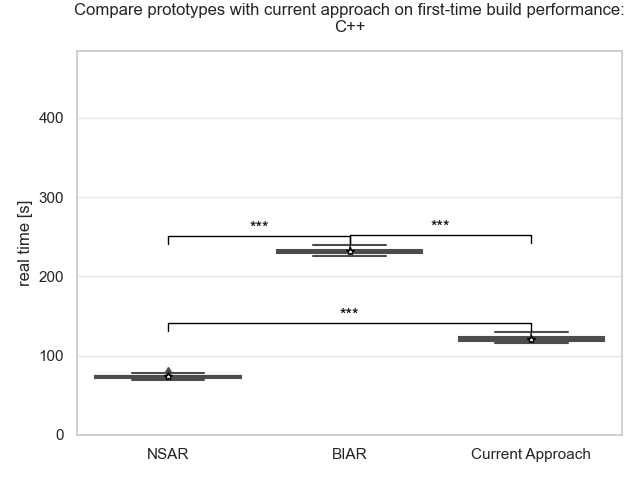
\includegraphics[width=0.87\textwidth]{thesis/graphics/compare-plots/compare_prototypes_with_current_approach_on_first-time_build_performance:_c++.png}
      \caption{\texttt{C++} environment}
      \label{fig:prototypes-vs-current-first-time-build-cpp}
    \end{subfigure}
    
    \vspace{1em}
    \begin{subfigure}{\textwidth}
    \centering
      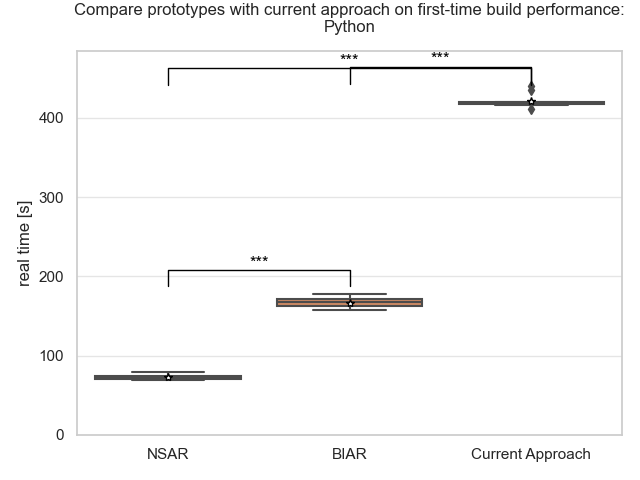
\includegraphics[width=0.87\textwidth]{thesis/graphics/compare-plots/compare_prototypes_with_current_approach_on_first-time_build_performance:_python.png}
      \caption{\texttt{Python} environment}
      \label{fig:prototypes-vs-current-first-time-build-python}
    \end{subfigure}
    \caption{First-time build performance of all approaches compared. Remarks: NSAR = nix-shell at runtime, BIAR = build image at runtime, * = a higher number of stars(*) indicates a greater statistically significant difference.}
    \label{fig:prototypes-vs-current-first-time-build}
\end{figure}

\subsection{Subsequent-time build}\label{subsequent-time-build}
The subsequent-time build (startup) performance -- start an environment container with a previously built configuration $C_{result}$ -- implies that the build-cache is full. The same argumentation for the network access holds as in the first-time build (see \ref{first-time-build}), and we explain how we measured the build time for each approach next.

In the BIAR approach, we assume that the environment image is available on the local container engine host since it has been previously built. The only step we need to do is start the right image inside a container. We find the correct image to start from the given $C_{result}$ by computing the hash over the configuration files before starting the container. 

The NSAR approach assumes that the store of the environment image has all derivations of the configuration installed. The execution flow follows: start a container from the environment image and run the cached nix-shell, which can instantly start the environment shell.

For the current approach, we assume that the environment image is available on the local container engine host. We start the image as a container, and the environment is ready. 
\paragraph{Prototypes compared with each other}
\begin{figure}[h!]
  \centering
  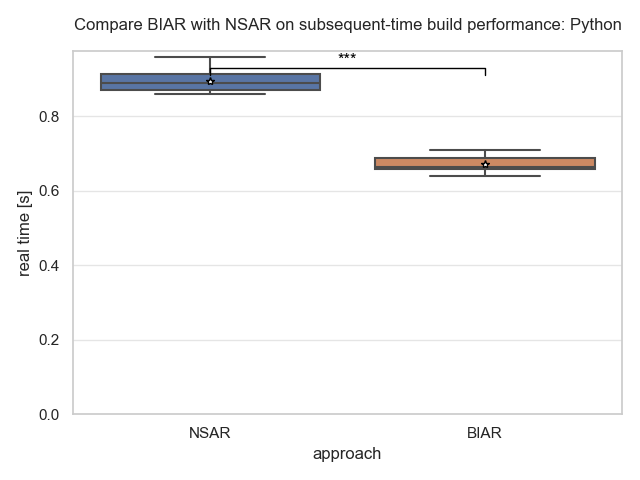
\includegraphics[width=0.74\textwidth]{thesis/graphics/compare-plots/compare_biar_with_nsar_on_subsequent-time_build_performance:_python.png}
  \caption{Comparing the measurements of our prototypes' subsequent-time environment startup performance using the Python environment. Remarks: NSAR = nix-shell at runtime, BIAR = build image at runtime, * = a higher number of stars(*) indicates a greater statistically significant difference.}
  \label{fig:nsar-biar-subsequent-time-build-python}
\end{figure}
We can see in figure \ref{fig:nsar-biar-subsequent-time-build-python} that BIAR is significantly faster than NSAR. BIAR takes between 0.65 and 0.7 seconds, whereas the NSAR startup time lies in the time range of 0.85 to 0.95 seconds. Since both have similar results, we can restrict ourselves to the \verb|Python| environment. This difference is incurred mainly because the NSAR prototype must check if the cache can be reused for the nix-shell execution and bind mounts two additional directories into the container. It also needs network access, which adds overhead as it requires Docker to add network configuration at the environment startup. 

\paragraph{Prototypes compared to current implementation}
The current approach has a startup time of around 0.6 seconds which is significantly faster than both prototypes (around 300ms faster than NSAR and 100ms faster than BIAR). This result can be observed in figure \ref{fig:subsequent-time-build-cpp} and is analogous to the \verb|Python| environment. We already provided some likely causes why NSAR is slower than BIAR. One reason for the difference between BIAR and the current approach might be the former's MD5 hash value computation over the configuration before starting the environment.

\begin{figure}[h!]
  \centering
  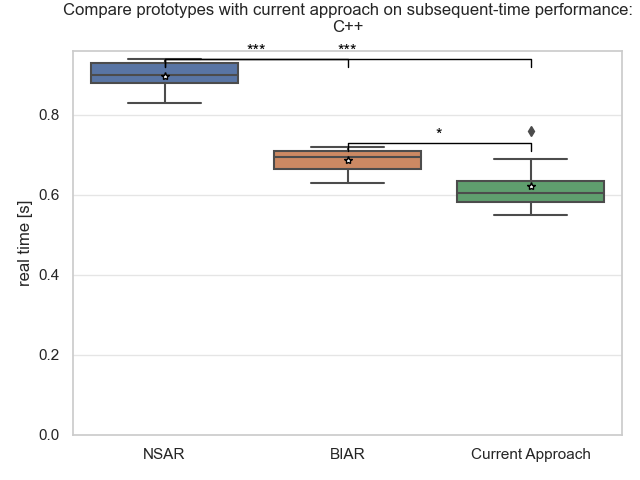
\includegraphics[width=0.8\textwidth]{thesis/graphics/compare-plots/compare_prototypes_with_current_approach_on_subsequent-time_performance:_c++.png}
  \caption{Comparing the measurements of our prototypes' subsequent-time environment startup performance to the current approach using the \texttt{C++} environment. Remarks: NSAR = nix-shell at runtime, BIAR = build image at runtime, * = a higher number of stars(*) indicates a greater statistically significant difference.}
  \label{fig:subsequent-time-build-cpp}
\end{figure}

%\subsection{Scalability}
%We want to benchmark how ``scalable'' an approach is in terms of growing disk space usage as the number of environments users use increases. As each environment in our  

\section{Security}\label{results-security}
The security of an environment is essential as we want to restrict users from breaking out of their isolated container to prevent attacks on the host system or other users' environments. At the same time, we want to provide a controlled and isolated environment to each user for remote code execution because we are in the context of a cloud IDE. 

We assume in this section that beyond the prototype-specific implementation, an environment is implemented such that exploits are made as hard as possible (e.g., remove privileges and access to the kernel). Under this assumption, the current approach is less likely to have security vulnerabilities. 

We discuss the two main attack vectors, the shared cache and network access for both prototypes, and how they could lead to security vulnerabilities. We outline ideas for preventing these vulnerabilities with potential implementations in the further work (see \ref{restrict-network-security} and \ref{improve-shared-cache-security}).

The BIAR prototype is generally vulnerable to attacks from the lecturers as the builder container has both attack vectors. In contrast, the NSAR prototype is vulnerable to attacks from any user since every user interacts with the environments with both attack vectors.

The environments produced by the BIAR prototype have no security vulnerabilities inherent to the implementation. Other vulnerabilities may exist that are not a direct result of our implementation -- for example, insecure packages. We can remove access to the network for each environment, and there is no shared component between containers. 
\subsection{Shared cache attacks}
We divide this section of cross-cache attacks into the two types of shared caches: the Nix store and the nix-shell cache. The latter is only applicable to the NSAR prototype.
\paragraph{Cross-cache attacks on the Nix store}\label{cross-cache-attacks-on-nix-store}
The Nix store cache is vulnerable to denial-of-service (DoS) attacks. For example, a malicious user could fill the cache with garbage derivations until the VM runs out of memory.

In addition, the shared Nix store is possibly vulnerable to cache poisoning. A user can put invalid entries (derivations) into the cache, which another environment container could access and deem valid. For example, a malicious user could construct a derivation that has as directory name the hash of a popular package $p$ and put it inside the store. If a configuration specifies this package $p$ in some following build process, then Nix will use the faulty cached derivation from the shared Nix store.

In our prototypes, the Nix database is also shared. It keeps track of the mapping between dependencies and derivations in the Nix store and can be arbitrarily modified to remap dependencies between derivations. One result is that the database becomes out of sync with the Nix store. Thus the database needs to be rebuilt by Nix if it cannot use the mappings from the database, which degrades performance and could even result in DoS. 

Possibly, the lecturer could introduce unintended security vulnerabilities to an environment, for example, by misconfiguring a package or using a malicious package. It is generally the responsibility of the lecturer to configure an image correctly, but these unintended attack vectors could compromise the Nix store. Nix employs defaults that prevent packages’ installation from the Nixpkgs collection based on the package metadata. Nix will not install a package if its meta value indicates that it is broken, does not run on the given system, or has known security vulnerabilities. 

The multi-user feature (see \ref{Nix-multi-user}) makes some security vulnerabilities harder to exploit (e.g., cache poisoning). This is because the root owns the Nix store and database, and builds are performed by a daemon, preventing arbitrary builds. Thus a user may need root permissions to access and change part of the Nix store and database. However, multi-user mode does not help with other attacks like DoS on the Nix store and does not improve the vulnerable nix-shell cache. The reason for this is that this feature is devised to share the Nix store across multiple user accounts to prevent cross-user attacks, but not share the Nix store across environment containers that all have the same user.
\paragraph{Cross-cache attacks on nix-shell cache}\label{cross-cache-attacks-on-nix-shell-cache}
Environments in the NSAR prototype share two caches, one for the Nix store and the other for the nix-shell. The NSAR approach needs both caches to achieve fast startup times for subsequent environment builds. 

The same security vulnerabilities as for the shared Nix store potentially exist for the nix-shell cache, which currently has no barriers against cross-cache attacks. This is because the files inside the nix-shell cache are writable by the user, unlike the files in the Nix store, which are read-only. Thus a user could quickly delete the cached files, which delays other environments’ startup time, or change the files in arbitrary ways. An example of the latter is changing the symlink of the \verb|nix-shell |’s derivation so that it points to another derivation in the nix store.

\subsection{Network access attacks}\label{security:network-access-attacks}
Each builder container of BIAR or environment of NSAR has access to the public network, mainly to provide the nix-shell access to the binary cache (cache.nixos.org) to download prebuilt packages not already in the Nix store. Another reason to provide network access would be to allow the use of ``fetcher'', which Nix provides to fetch source code from repositories like Github, Gitlab, or PyPI \cite{NixFetchers}. These fetchers are needed if users want to, for example, build specific versions of packages from source code that are not available in the Nixpkgs collection.

Unrestricted network access is problematic as it would allow a user to potentially fetch arbitrary sources such as code repositories or web pages. This broad access would make it significantly easier to execute malicious code remotely to attack the cloud system or, for example, use the computing resources for adverse purposes. Another thing to remark is that in the particular use case of CodeExpert, students are not allowed to access the network, for example, during programming exams. This case is not a security vulnerability per se but a requirement that must be satisfiable for our prototype to be used in this context.

%To summarize this security evaluation, the BIAR prototype has fewer security vulnerabilities than the NSAR one.

\section{User experience}\label{result:UX}
To evaluate if our prototypes boost the flexibility in coding exercises, we evaluate the user experience compared to the current solution. The lecturer must set up the coding environments first such that students can run coding exercises in the environments. Therefore this section covers the process, flexibility, and wait time for setting up a configuration. Additionally, it looks at students' interaction response time for environment startups. %For this section, the user of the BIAR prototype is the lecturer, and the user of the NSAR prototype are all users. 

We define a ``good'' user experience in our context with the following properties that are influenced by the ``user experience'' (UX) concept described in \cite{fagerholm2012}.
\begin{enumerate}
	\item Ease of writing configurations
	\item Flexibility of setting up environments with any language and packages
	\item Efficient change of configurations, which includes the build time of the configuration
	\item Quick environment startup times for subsequent environment startups
\end{enumerate}

\subsection{Configuration}\label{user-experience-config}
We first cover the identical arguments for our prototypes because both use Nix as a build system. With the BIAR and NSAR prototypes, the lecturers can directly specify all environment packages themselves (without interacting with the developer) by changing one of the configurations of $C_{preset}$. Such a configuration has a fixed interface (see \ref{prototype-configuration}) for increasing the ease of use when writing configurations. Changing the configuration for lecturers that only specify packages from the Nixpkgs collection is trivial, as the lecturers do not need to learn the Nix language. To showcase the ease of specifying and changing the configuration, one can look at the \nameref{preset-python.nix} configuration and compare it to the \nameref{changed-python.nix} configuration. The \nameref{preset-python.nix} is a reduced example from $C_{preset}$. One Python package and two other packages have been added as highlighted in \nameref{changed-python.nix}.
\definecolor{light-gray}{gray}{0.75}
\begin{lstlisting}[caption={preset-python.nix}, title={preset-python.nix}, label={preset-python.nix}]
{ pkgs }: with pkgs;
let
  pythonEnv = python39.withPackages (p: with p; [
    numpy
  ]);
in
{ inputs = [ pythonEnv ]; }
\end{lstlisting}
\begin{lstlisting}[caption={changed-python.nix}, title={changed-python.nix}, label={changed-python.nix}, escapechar=!]
{ pkgs }: with pkgs;
let
  pythonEnv = python39.withPackages (p: with p; [
    numpy
    !\colorbox{light-gray}{networkx}!
  ]);
in
{ inputs = [ pythonEnv !\colorbox{light-gray}{openssl}! !\colorbox{light-gray}{sqlite}! ]; }
\end{lstlisting}
If the lecturer wants to specify a custom package or package version, then he needs to learn some details of the Nix language for declaring the package as a derivation. Specifying a custom derivation can be challenging, but there are many examples in the Nix documentation (e.g., \cite{NixPythonGuide}) which should provide ample resources for this task. With some packages and languages, the lecturer may need to figure out which environment variables need to be set at runtime, e.g., such that the compiler finds the shared libraries for linking. This can be challenging, but there are many examples of typical use cases in the Nix documentation, e.g., in \cite{NixPythonGuide}. The NSAR prototype makes the specification and restriction of global environment variables inside the shell easy and has a \verb|shellHook| attribute in the configuration interface for this purpose. This specification and restriction of environment variables may be more challenging with the BIAR prototype as environments do not have the \verb|nix-shell| functionality. Special attention is needed when configuring interpreted language using our prototypes. Nix wraps one interpreter and other executables together such that they can find each other and all of the modules. Thus Nix only allows one of these wrapped environments to be installed globally since they otherwise conflict with the interpreter to load out of the PATH environment variable \cite{NixPythonGuide}.

In the current solution, the lecturer cannot deploy the configuration changes directly and must contact the developer to deploy every (minor) change in the configuration. This process can sometimes be advantageous for the lecturer since the developer is responsible for making the images run correctly in production. On the flip side, it may also happen that the developer cannot make a (small) configuration change requested by the lecturer as it may be, e.g., too tricky. If the lecturer does not want to use a predefined configuration, he can write his custom configuration or extend a predefined configuration. This requires knowledge of writing a \verb|Dockerfile| \cite{CXDocs}. Unlike our prototypes which allow the composition of configurations, in most cases, the lecturer cannot easily compose two different configurations written as \verb|Dockerfile|'s into one image in the current solution as argued in \ref{reproducibility-docker-build}.

\subsection{Flexibility}
The current solution restricts the lecturers to packages and specific versions that are available in the used Linux distribution, such that it may happen that a package requested by the lecturer is not available for installation. With our prototypes, lecturers can choose from over 60'000 predefined packages from the Nixpkgs collection or declare any custom package or version they need. This is because Nix can build a package from source code by fetching this code from remote code repositories. The result is almost unlimited flexibility for configuring the environment. 

\subsection{Wait time for user interactions}
This section discusses the time the user must wait until different interactions (e.g., changing the configuration) are complete with our environments. 

The faster the build time, the quicker the lecturer can iterate over configurations during development and when changing the configuration, which improves the UX. Therefore we use the results from \ref{prototypes-vs-current-first-time-build} to evaluate the efficiency of configuration changes. The build time for BIAR is approx. between 2 and 4 min, which is slower than NSAR, which takes around 1min for a complete build with empty caches. Note that after some packages have been built, the build caches are unlikely to be empty, and the build times tend to be faster. Furthermore, both of our approaches allow us to significantly optimize the first-time build performance with a seeded store in the case of NSAR (see \ref{results-seeded-nix-store}) and in the case of BIAR see \ref{optimize-build-and-push-BIAR}.

The current solution has a bit faster build time than BIAR but is slower than NSAR. However, with the current solution, the lecturer only reaches these build times when testing the environment on a local machine. In contrast, our approaches allow direct testing on production systems after the above build time. To test a configuration change with the current approach in the cloud system, the lecturers must contact the developer. Then he must wait potentially many days until the developer has deployed the corresponding image to use it.

The other primary user interaction with our environment that incurs wait time is when a student wants to run coding exercises. In this case, the first student who starts an environment from a new configuration must wait longer, whereas all following students experience the subsequent startup time. Since students invoke an environment startup many times for each job execution, the faster the subsequent startup time, the better the UX. Note that the current solution is faster than BIAR, which is faster than NSAR (see \ref{subsequent-time-build}). 

%TODO: maybe include this in the discussion?
%\subsection{Security of builds and environments}
%Students who run code inside environments and lecturers who configure coding exercises are interested in secure environments and isolated builds from other users, respectively, for a good UX. As argued in section (\ref{results-security} this property is not satisfied for any user in the NSAR prototype nor for the students in the BIAR prototype.

To summarize the UX of the lecturer, our approaches have advantages in configuration, flexibility, and build time over the current solution. On the other hand, the current solution has the edge in the subsequent startup performance for students. 

\section{Developer experience}\label{result:DevX}
In this section, we evaluate the developer's experience in maintaining and developing the implementation of our prototypes compared to the current approach.

We define a ``good'' developer experience for our problem with the following properties influenced by CodeExpert developer's feedback and the developer experience defined in \cite{fagerholm2012}.
\begin{enumerate}
	\item Minimal workload from configuration changes by the lecturer
	\item Less responsibility for usage defects
	\item Ease of development and testing 
	\item Minimal maintenance of implementation (e.g., images and dependencies)
	\item Increase robustness of the cloud-based system.
\end{enumerate}

\subsection{Developer involvement with configuration changes}
Ideally, the developer does not need to be involved whenever a lecturer submits a new or changed configuration for deployment on the production systems. This goal minimizes the developer's workload and is fulfilled with our prototypes. This stands in contrast to the current approach, where the developer needs to be in direct contact with the lecturer and perform the following manual steps
\begin{itemize}
	\item check if the requested packages are available for installation,
	\item figure out how these packages need to be installed,
	\item if they can be installed without much difficulty, then build and then test the image,
	\item and if all the above steps are successful, deploy it to the image registry.
\end{itemize}

Another critical point is that our approaches shift the responsibility for setting up a correct and secure image (e.g., not using broken or vulnerable packages) from the developer to the lecturer. This argument follows from the above argumentation, where we outline the impact of a configuration change on a developer. 

\subsection{Development and testing}
With our prototypes, a developer can easily add, e.g., a new language as a configuration to the $C_{preset}$ group by writing a new template as a Nix expression. This template can then be used or customized by a lecturer. At the moment, adding a new predefined configuration means writing a custom \verb|Dockerfile| and then manually building it and deploying it to the production system, which can be cumbersome.

The developer needs to learn how Nix works and its domain-specific programming language to implement our prototypes, develop them further and test them. Learning Nix can be challenging since it is a purely functional programming language with limited documentation and usage examples. Nix also differs from other functional programming languages such as Haskell. It is often unclear what the ``standard'' Nix approach for a common problem is. However, it is generally advisable to use and compose the many predefined helper functions from the standard library. To aid with development, Nix provides a repl tool that is useful for trying out small Nix code examples and the nix-shell that allows for incremental builds and debugging inside the build-environment (see \ref{nix-shell&nix-build}). 

Nix provides tools that make debugging more manageable: the nix-shell sets up the build environment that can be debugged and inspected and from which the developer can build the package or image manually. Testing container images is best done in a continuous integration (CI) pipeline by, for example, building the reproducible images and then running tests specified, e.g., with a bash script. The primary tool to aid with CI and testing in the Nix ecosystem is Hydra (see \cite{Hydra}), which can cache CI builds and make subsequent pipeline runs faster. Furthermore, testing one or two base images of our approaches that rarely change is likely less of a burden to the developer than testing more than a dozen, each with different languages, in the current approach. 

\subsection{Maintenance}
For the NSAR prototype, the developer only needs to maintain a single image, i.e., built with Nix. However, the Nix store needs maintenance as the developer needs to run the garbage collection or store path optimization regularly to avoid running out of disk space. When the developer runs the garbage collection tool of the Nix store, it is essential not to remove potential configuration files (e.g., shell scripts) stored in the Nix store. These files are needed for the container at runtime. Additionally, the nix-shell cache could need maintenance for the NSAR prototype. 

The NSAR prototype has the \verb|cached-nix-shell| package as a dependency, a Nix package developed by the community that needs to be updated by the developer and might break after an update. Adding features to this package or making changes might make maintaining this dependency a burden. However, our prototypes have much fewer dependencies to maintain than the current approach, which has many packages in multiple image configurations with different package managers such as pip and DNF. The fewer dependencies our prototypes have on external packages, the better the developer experience.

The BIAR prototype has two images that the developer needs to maintain and a shared Nix store, where the same arguments apply as described for the NSAR prototype. Because the BIAR prototype builds an image for every unique configuration, the image registry likely becomes overloaded with many images. Therefore it is necessary to remove images from the registry regularly. It would be best to remove the least used images to prevent unnecessary rebuilds, but this would require collecting image usage statistics.

Our prototypes use a specific version of Nixpkgs and Nix, which needs to be updated in the future and would require a rebuild of the images. For the current prototypes, updating the Nix version would imply updating the Nix base image from Docker Hub. Updating the Nixpkgs version is handled using the Nix package \verb|niv|.

It is crucial for an approach's development and robustness that the same build inputs lead to the same output in future builds. The builds of both prototypes produce the same output because they are reproducible, except if the developer changes the configuration or script files that are copied into the image or bind-mounted into the environment. On the other hand, the current approach is not reproducible since the image builds can fail (see \ref{reproducibility-docker-build}). %Furthermore, the current approach has many images which need to be maintained and updated, resulting in a worse developer experience. 

%The developer is interested in the secure implementation of an approach to prevent attacks on the host system. This property is currently not fully satisfied by both of our prototypes, but the BIAR prototype has the advantage over the NSAR prototype. 

%Interpretation of the research results
%Comparison of the results with those of the previous studies
%Contributions of your research to the existing knowledge body
%Limitations of the study
%Unexpected results
%How the results support or refute a certain theory or findings of the previous studies

%Opinionated discussion about the results
%Provide argumentation for 
\chapter{Discussion}\label{discussion}
After presenting the results in the last chapter, this chapter will interpret the results to propose the best approach for solving our problem. 

\section{Performance results}\label{discussion:performance}
This section discusses the performance criteria results presented in the last chapter. The measurement process we used for the performance results produces relevant results for our problem. The reason is that we benchmark with a ``warmup''-phase on a virtual machine architecture (see \ref{methods-for-data-collection}) to simulate the conditions of a running cloud-based IDE. To compare the performance of different approaches, we tried to measure the execution beginning from identical start-points and ending at the same result (outlined in \ref{results:performance}) and with about the same packages installed (see \ref{appendix:bench-envs-packages}) to get comparable results. 

We can summarize from the BIAR approach-specific benchmarks results that saving I/O operations and disk/cache space tends to pay off in the first-time build performance for the streamed build strategy. According to the Nix documentation, we assumed that the streamed strategy saves I/O operations and disk/cache space. We could make a stronger argument if we verified this assumption specifically with benchmarks. As expected, the subsequent-time build performance did not result in statistically significant differences between both strategies since Nix uses the cached layers and does not rebuild for both strategies. Therefore we should opt for the streamed strategy implementation.

For the NSAR approach, we can conclude that the results matched our expectations. This implies that we should use a cached nix-shell, and we could use a seeded Nix store from a performance standpoint to improve the first-time build. The cached nix-shell is slower for the first-time build performance than the uncached nix-shell, but this is not problematic since we can be slower in this case. The cached nix-shell allows us to achieve an up to three times faster subsequent-time startup compared to not using caching. This result is somewhat similar to the very limited data (of an unknown measurement process) of \cite{CachedNixShell} where a slighter difference was measured between the cached and uncached nix-shell. 

The results of the seeded store evaluation also indicate that adding a few packages, which are available in the binary cache, to a previously built configuration results in a small overhead compared to the first-time build. This result infers that Nix can efficiently cache previous builds in the Nix store and also transfers to the BIAR prototype since Nix efficiently caches both the nix-shell execution and the resulting layers of an image build as derivations in the Nix store (see \ref{hermeticity}, \ref{efficient-caching-of-layers}).

Recall that in \ref{results-seeded-nix-store}, we measured a more negligible overhead when building six additional packages in the Python environment that were not in the seeded store than building one package in the \verb|C++| configuration change. This result is unexpected since we predicted the opposite. The reason for this result could be that the dependencies of the additional six packages have a large intersection with the dependencies of packages already in the seeded store. This would confirm our expectation outlined in \ref{BIAR-execution-flow} and aligns with the argumentation of \cite{Christensen2018}. However, we can not make a decisive argument since the packages added to each environment are different and, obviously, the environments themselves (see \ref{test-environments}). 

To summarize, even though the seeded Nix store improves the first-time build, it does not provide a strong enough argument to justify its implementation for our problem. This is because, after a first-time build, the resulting Nix store is comparable to a seeded store from the viewpoint of subsequent builds with small configuration changes. Our argument makes sense for our problem since suppose a running cloud-based IDE in which we provide configuration templates that most lecturers will not change or only slightly. Then after the first build, which produces a ``seeded store'', all other lecturers' configuration changes will only experience a small overhead.

This discussion on the NSAR implementation has implications: caching the nix-shell is required to achieve fast environment startups for subsequent-time invocations, and implementing a seeded Nix store is unnecessary. The former implies that we must implement the unsafe shared nix-shell evaluation cache (see \ref{cross-cache-attacks-on-nix-shell-cache}). %We will use the idea of a seeded store in the further work discussion.

The first-time build performance of the NSAR prototype is the fastest among all three approaches (see \ref{first-time-build}) and even can be optimized with a seeded store, as argued before. The prototype of the BIAR approach has a comparable first-time build performance to the current approach, as argued in the \verb|C++| environment results of \ref{prototypes-vs-current-first-time-build}. Unlike the current approach, the BIAR and the NSAR prototypes automatically optimize the build time for small configuration changes, but in the case of BIAR, this optimization is currently limited by the push-time as discussed in \ref{biar-approach-specific}.

The results of the subsequent-time build performance were as expected. The overhead measured for checking the nix-shell cache (300ms) in the NSAR prototype align with the, again, very restricted result (290ms) from \cite{CachedNixShell}. This overhead is roughly three times the time it takes to compute the hash value over the configuration in the BIAR prototype. This hash value computation might also be the difference in the subsequent startup performance between the BIAR prototype and the current approach since they both start a container without a network and without checking cached results like the NSAR prototype. This means that it is essential for our problem to optimize the cache verification in the NSAR prototype and the hash value computation in the BIAR implementation. The cache verification is challenging to optimize as it is already optimized and an external package outside our prototype implementation. 

%TODO: scaling
In our benchmarks, we used two test environments: a \verb|C++| -- to represent compiled languages -- and a Python one -- to represent interpreted languages. We wanted to evaluate whether one approach is more suited for one environment than the other or if they perform equally well regardless of the environment. Our results from \ref{first-time-build} and \ref{subsequent-time-build} imply that no approach is more suited to one type of environment over the other. 

\section{Security results}\label{discussion:security}
The shared cache attack vector results showed that the NSAR prototype has more security vulnerabilities than the BIAR prototype for two main reasons. The first, apart from the shared Nix store, is the additional cache for part of the nix-shell execution. This cache has no barriers against cross-cache attacks, resulting in security vulnerabilities or performance degradation for other users. The second is due to a reasonable assumption in our context that the lecturers have no intention to maliciously attack the system since they configure the environments for teaching purposes. This assumption holds for the network attack vector as well. 

Another point is that the shared cache security vulnerability could easily be removed from the BIAR approach by just removing the shared Nix store from the builder container without impacting the subsequent-time build performance. The implication would be that the build performance for configuration changes would equal the first-time build with empty build caches. This quick-fix would tradeoff performance for security. This stands in contrast to the NSAR prototype, where the shared Nix store and shared nix-shell cache is required to achieve the essential quick subsequent time environment startup. Therefore the BIAR prototype has even more advantages from a security standpoint than the NSAR prototype.

As argued in \ref{cross-cache-attacks-on-nix-store}, installing Nix in multi-user mode would improve the security of the shared Nix store to a small extent. This would, however, come at the cost of needing to run the Nix daemon inside each environment and configuring custom \verb|systemd| initialization mechanisms \cite{NixMultiUser}. The former could result in performance degradation and the latter in poor developer experience. Therefore we conclude that the implementation tradeoffs prevail over the security gains for implementing the multi-user mode.

To summarize, the security vulnerabilities of both prototypes have their cause in which part of the prototype's architecture the Nix build system is installed. Since the resulting environments of the BIAR prototype and obviously of the current approach do not have Nix installed, the environments do not have a shared cache nor network access and therefore have none of the two attack vectors. This contrasts with the NSAR approach, where the environment needs to have Nix installed.
% network access, -> exam situation
\section{User and developer experience results}\label{discussion:UX-and-DevX}
The results are based on our analysis of the prototypes and current approaches implementations based on the enumerated properties of what we define as a ``good'' user or developer experience. For the developer and user experience results, we do not have results from previous studies for comparison. This is because of our particular use cases in the context of a cloud-based IDE where we have developers on one side and lecturers and students on the other. Each side has individual requirements on the system and challenges with the current approach. 

\subsection{User experience}\label{discussion:UX}
From the results of \ref{user-experience-config}, it seems that our prototypes have a slight advantage. However, we cannot decisively conclude if they provide an improved UX over the current approach regarding the ease of writing configurations. Indeed they have the edge for composing configurations and for simple configuration changes, considering the challenge of writing a custom \verb|Dockerfile| for the current approach. However, whether the advantages outweigh the fact that the lecturer needs to take on more responsibility with our prototypes is unclear. Furthermore, some details -- e.g., figuring out the correct environment variables -- of configuring custom configurations with Nix could be more or less challenging. To make a more decisive argument, testing the configuration process of our prototypes with lecturer feedback would be beneficial.

Regarding boosting the flexibility of configuration, our prototypes clearly have the edge over the current approach. Users can efficiently change the configuration with our prototypes and test the effects on the production systems within a few minutes instead of possibly multiple days for the current approach. Since the subsequent startup time of the current approach is slightly faster than BIAR and much faster than NSAR, the UX for executing code in environments tends to be better for the current approach. To make a more decisive argument in this case, we would need to test our prototypes with student feedback to find out whether, e.g., the small startup overhead of the BIAR prototype compared to the current approach impacts the user experience poorly. 

\subsection{Developer experience}\label{discussion:DevX}
The developer's workload from configuration changes by the lecturer is undoubtedly minimized for our prototypes as opposed to the current approach, where configuration changes are likely to be very demanding. Our prototypes also have the advantage over the current approach as the developer has less responsibility for usage defects if the lecturer does not set up the environment correctly. Thus our approaches have a much better developer experience for both points. 

The further development and testing of our prototypes can be challenging initially. However, it is hard to make a powerful argument on how much the tools provided by Nix for development and testing alleviate the ease of implementing and developing our prototypes compared to the current approach in the long run. Feedback from developers who worked with the prototypes would help make a more solid argument for this aspect.

Our prototypes have one or two base images and few dependencies to maintain, resulting in a better developer experience than the current approach. The advantage of our prototypes might shrink from maintaining the Nixpkgs and Nix versions, the shared Nix store, the nix-shell cache (for NSAR), and the image registry (for BIAR). Maintaining the nix-shell cache and additional dependency (\verb|cached-nix-shell|) of the NSAR prototype likely overweighs the burden of the BIAR prototype's additional image and image registry. Our prototypes offer more robustness and are future-proof as they are reproducible.
%To summarize, the maintainability for the developer is better for our prototypes compared to the current approach.
\renewcommand{\arraystretch}{2}
\chapter{Conclusion}\label{conclusion}
In this thesis, we found two feasible approaches to building images at runtime based on the lecturer configuration, described the implementation of the prototypes for each solution approach, and evaluated our prototypes and the current approach to arrive at a comparison among the evaluation results. 

\section{Proposition}
The final aim of this thesis is to propose the best approach based on the results and discussion. To this end, we summarized the quantization results of each evaluation criteria in table \ref{table:conclusion-overview}. Each cell in the table is a real number from the interval $[0,\;1]$, where higher values represent a more relevant result for a criterion. We describe how we reach these points in \ref{appendix:conclusion-point-assignment}.

\newcolumntype{x}[1]{>{\centering\let\newline\\\arraybackslash\hspace{0pt}}p{#1}}
\begin{table}[h!]
\centering
\begin{tabular}{|m{3.2cm}|cccc|c|}
\hline
\textbf{Evaluation criteria or approach} & \textbf{Performance} & \textbf{Security} & \textbf{UX} & \textbf{DevX} & \textbf{Total} \\ [1ex] \hline
\textbf{NSAR approach}    &  0.45       & \textcolor{red}{0}   &  \textcolor{green}{0.75}      & \textcolor{green}{0.9}    & 2.1                           \\ [0.5ex] \hline
\textbf{BIAR approach}    & 0.6    & \textcolor{green}{0.8}               & \textcolor{green}{0.75}    &  \textcolor{green}{0.9}    & \cellcolor[HTML]{AAACED} 3.05                       \\ [0.5ex] \hline
\textbf{Current approach} & \textcolor{green}{0.75}        & \textcolor{green}{1}         &  \textcolor{red}{0.35}        & \textcolor{red}{0.1}     & 2.2                     \\ [0.5ex] \hline
\end{tabular}
\caption{Approaches are compared with each other based on the results of \ref{appendix:conclusion-point-assignment}. Note that the BIAR approach has the highest point total. Remarks: UX = user experience, DevX = developer experience}
\label{table:conclusion-overview}
\end{table}

To conclude, we propose the BIAR approach, as it has the highest point total and is more suited for our problem than the NSAR approach, which, although radical and lightweight, is unacceptable from a security standpoint. The BIAR approach has the potential to alleviate many tradeoffs of the current approach, e.g., by improving the flexibility of the users and the developer experience.

The BIAR approach could be used as a basis to implement the next version of the cxEnvironments for CodeExpert. Due to the design or our approaches that respect the current architecture and execution flow, the proposed approach can potentially be made available to lecturers in parallel to the current approach, such that existing cxEnvironments will continue to run, and newly created environments will use the latest advantages of the proposed approach.

\section{Further work}
After having answered our problem statement by proposing a prototype that solves our objective, we turn to describe future work in this section.

\subsection{Testing prototypes with user feedback}
As we have argued in some parts of \ref{discussion:UX-and-DevX}, testing our prototypes with user feedback is important. These tests could, for example, include:
\begin{itemize}
    \item How difficult it is for lecturers (knowledgable or not) to configure environments to test the configuration experience.
    \item What configuration parameters are needed such that the lecturer can configure environments (to determine the configuration interface of our prototypes).
    \item What is the impact on the UX for students caused by the potential additional startup time of our prototypes compared to the current approach.
\end{itemize}

\subsection{Custom package collection}\label{custom-package-collection}
It would make sense to add a custom Nixpkgs extension (see \ref{nix-tools-package-management}) for CodeExpert, such that, for example, the developer and lecturers can share custom tools that every lecturer can use in configurations. This would allow the lecturer to improve coding exercises' debugging or testing functionalities for students. Another use case is if developers and lecturers need to override the default configuration for some package, e.g., to fix a package bug or add environment variables needed for our context. 

This private package collection can be achieved using \emph{overlays} i.e., a method to change and extend Nixpkgs \cite{Overlays}. The overlay could be built regularly in a CI pipeline using the Nix CI tools \cite{Hydra}. Then the builder container or environments for the BIAR and NSAR prototypes, respectively, could use this extended package collection by just adding it as a channel.

\subsection{Optimize build and push time for BIAR approach}\label{optimize-build-and-push-BIAR}
The optimization of the subsequent-time build performance of the current BIAR prototype is limited by the push time as seen in \ref{biar-approach-specific}. To overcome this limitation, we could try to avoid pushing layers that are already available on the image registry. This idea makes sense since images can share common layers according to the OCI image specification. Furthermore, the shared dependencies of packages likely result in their own layer when building images with Nix (see \ref{efficient-caching-of-layers}). Nix can efficiently cache these layers (see \ref{discussion:performance}). A Nix library exists as a package (see \cite{Nix2Container}), which is a promising solution to our problem. The limited benchmarks outlined in \cite{Nix2Container} provide some intuition on the order of magnitude the build and push time could improve.

%Another idea would be to create an image registry (i.e., on a separate VM) that has Docker installed and builds an image based on the given configuration hash if it has not already been built before or serves the locally cached image. This proposition would circumvent the need to push images to a registry, and this new registry can use the Nix build caching. 

\subsection{Improve security of shared cache}\label{improve-shared-cache-security}
To improve the security of the shared Nix store in the BIAR and, more importantly, the NSAR prototype, we present one possible implementation idea. 

We can use an overlay filesystem (e.g., \verb|OverlayFS| \cite{OverlayFS}), also called union filesystem, similar to the way Docker shares layers between images (see \ref{images-and-layers}). A read-only snapshot of the shared Nix store cache is mounted into the container (i.e., at \verb|/.nix-store-cache|). We then overlay-mount this cache (using the overlay filesystem) into \verb|/nix/store| where Nix expects the cache to be with a read-only snapshot of \verb|/.nix-store-cache| as the ``lower'' directory and a user-writable directory (e.g., \verb|/nix/store/upper|) as ``upper'' directory. Now we have a similar result to \ref{containers-and-layers} and the user cannot modify the shared Nix store to attack the host system or other environments because each container has a copy-on-write view of the cache. This means that if the user modifies the cache by, e.g., performing builds, the accessed read-only files get copied to the upper directory, which is deleted when the container gets removed.

Before we take a snapshot of the shared cache, it is essential to preinstall the most popular packages analogous to the seeded Nix store. Then we can update the cache frequently with the most popular packages to keep the cache up to date. Determining the most popular packages would require gathering usage statistics, e.g., tracking which packages have been downloaded from the binary cache.

\subsection{Restrict network access and improve security}\label{restrict-network-security}
We present two ideas that can be used to circumvent the need to have a container with open access to the network, which results in security vulnerabilities outlined in \ref{security:network-access-attacks}. 

\paragraph{Private binary cache}
One can set up a private binary cache inside a local container and access it over the local network \cite{NixBinaryCache}. Apart from removing the need to access the public network, it would speed up the installation of packages by reducing the network roundtrip time. This private binary cache would require preinstalling most packages of the public one and frequent updates to keep the local cache up to date, which needs to be scheduled by a developer. A better solution that automatically takes care of the last two requirements would be to set up a binary cache inside the local network as a proxy of the public cache. This proxy fetches first-time accessed packages from the public cache and saves them for subsequent accesses on the local disk \cite{NixBinaryCacheProxy}.

\paragraph{Network traffic filter}
Another idea would be to restrict each container’s access to specific public IP address ranges, which are used, for example, by the public Nix binary cache CDN. To this end, we can filter the egress network traffic initiated from inside the container using a proxy HTTP-server connected to each container and restricting its outgoing requests. This proxy server would allow fine-grained control over which repositories and binary caches can be accessed, but the developer must configure them manually. 

\paragraph{Remove network access from environments}
Suppose no network connection is allowed for an environment. In that case, we can use the first idea of a local binary cache proxy to solve the problem of needing access to the public binary cache. If we want to allow fetchers for building custom packages, we could either make sure that these packages are cached in the Nix store from previous builds, or we could set up a custom package collection (see \ref{custom-package-collection}). If the lecturer wants to use fetchers, he must submit this package (i.e., as a Nix expression) to this package collection. The packages inside the collection must then be prebuilt before an environment can use them.

\appendix

\chapter{Appendix}
\section{Conclusion points assignment}\label{appendix:conclusion-point-assignment}
We outline in this section how we quantify the comparison of our approaches by assigning points to each approach for the qualitative results of the evaluation criteria. The points are real numbers of the interval $[0,\;1]$, where the highest possible point for each criterion is 1, and the lowest is 0. 

\subsection{Peformance}
%TODO: memory efficiency:
To quantize the performance discussion, we use weighted points listed in table \ref{table:performance-points} for first-time and subsequent-time performance categories. Since the maximum is $1$, the weights are chosen such that this maximum is attainable but cannot be exceeded. The best approach in a category gets the points in the first row, while the second and third-row looks at the relative difference to the best approach. What a ``small'' or ``large'' difference means is not rigorous and different for each category, i.e., a small difference for the subsequent-time build can be an order of magnitude lower than a slight difference for the first-time build. This is because the subsequent time build needs to be fast, and we penalize a difference to the best approach more. 

The approaches have the following point sums (in order of the categories in table \ref{table:performance-points}): 

\begin{itemize}
    \item NSAR: $0.35+0.1 = 0.45$
    \item BIAR: $0.25+0.35 = 0.6$
    \item Current approach: $0.1+0.65 = 0.75$
\end{itemize}
The assignment of each point is justified in the results and discussion sections (\ref{discussion:performance} and \ref{results:performance}).

\begin{table}[h!]
\centering
\begin{tabular}{||m{3.5cm}|| m{1.8cm}m{2.9cm}||} 
 \hline
 Category or \newline relative comparison & First-time build & Subsequent-time build \\
 \hline\hline
 Best approach & 0.35 & 0.65 \\ 
 Small difference to best approach & 0.25 & 0.35 \\ 
 Large difference to best approach & 0.1 & 0.1  \\ [1ex] 
 \hline
\end{tabular}
\caption{For each category, we assign points (real numbers in $[0,\;1]$) to an approach based on the relative comparison to the other approaches. There is only one ``best'' approach, and the others either have a ``small'' or ``large'' difference from this best approach.}
\label{table:performance-points}
\end{table}

\iffalse
\begin{itemize}
    \item NSAR: $0.1+0.3+0.1 = 0.5$
    \item BIAR: $0.1+0.2+0.3 = 0.6$
    \item Current approach: $0+0.1+0.6 = 0.7$
\end{itemize}
The assignment of each point is justified in the results and discussion section (\ref{discussion:performance} and \ref{results:performance}).

\begin{table}[h!]
\centering
\begin{tabular}{||m{3cm}|| m{1.8cm}m{1.8cm}m{2.2cm}||} 
 \hline
 Category or relative comparison & Memory-efficiency & First-time build & Subsequent-time build \\
 \hline\hline
 Best approach & 0.1 & 0.3 & 0.6 \\ 
 Small difference to best approach & 0.1 & 0.2 & 0.3 \\ 
 Large difference to best approach & 0 & 0.1 & 0.1  \\ [1ex] 
 \hline
\end{tabular}
\caption{For each category, we assign points (real numbers in $[0,\;1]$) to an approach based on the relative comparison to the other approaches, which means that there is only one ``best'' approach, and the others either have a ``small'' or ``large'' difference to this best approach.}
\label{table:performance-points}
\end{table}
\fi

\subsection{Security}
We quantize the security criteria with a penalty that gets subtracted from $1$ if the approach is vulnerable to a given attack target from a user group. We penalize attacks from students more than from lecturers (see table \ref{table:security-points}), for reasons discussed in \ref{discussion:security}. The weights are chosen so that each approach's worst or best assignment corresponds to the total maximum and minimum attainable points. From the discussion of \ref{discussion:security}, we conclude that the NSAR prototype is vulnerable to all attack targets and users and therefore gets $0$ points. The BIAR prototype is only vulnerable to attacks from lecturers and therefore gets $0.8$ points, whereas the current approach is safe and gets 1 point. 

\begin{table}[h!]
\centering
\begin{tabular}{||m{3cm}|| m{1.2cm} m{2.3cm}||} 
 \hline
 Attack target or user group & Host system & Other \newline environments \\
 \hline\hline
 Students & 0.4 & 0.4 \\ 
 Lecturers & 0.1 & 0.1 \\
 \hline
\end{tabular}
\caption{If an approach is vulnerable to a given attack target from a user group, then the penalty is subtracted from $1$. The result is the point assigned to the approach.}
\label{table:security-points}
\end{table}

\subsection{Developer experience}
For the developer experience, we assign weighted points to each property listed in \ref{result:UX} according to how ``important'' it is for the developer experience. The weights are chosen so that each approach's worst or best assignment corresponds to the total maximum and minimum attainable points.
Table \ref{table:devx-points} shows the points an approach receives if it fulfills the given property. In this case, it is not clear whether the approach fulfills the given property or not he receives half of the listed point. 

As mentioned in the discussion (see \ref{discussion:DevX}), the developer experience of the NSAR and BIAR prototypes is very similar for each property. Thus the point total is for both $0.9$ since they meet all properties except the third one (development and testing) since it is unclear if it is fulfilled. In contrast, the current approach has a total of $0.1$ as it does not satisfy any property except 3, where it is not fully clear whether this property is satisfied. 

\begin{table}[h!]
\centering
\begin{tabular}{||m{4cm}||ccccc||} 
\hline
 \textbf{Developer experience property number} & 1 & 2 & 3 & 4 & 5 \\
 \hline
 \textbf{Points} & 0.3 & 0.1 & 0.2 & 0.3 & 0.1 \\ 
 \hline
\end{tabular}
\caption{For each property, we assign points (real numbers in $[0,\;1]$) to an approach if it fulfills the property. The properties are listed at the beginning of \ref{result:DevX} and have the same enumeration order.}
\label{table:devx-points}
\end{table}

\subsection{User experience}
For the UX we assign weighted points to each property analogeous to the developer experience case mentioned above. Table \ref{table:ux-points} shows the points that an approach receives which is analogeous to the developer experience. The approaches have the following point sums (in order of the properties): 
\begin{itemize}
    \item NSAR: $0.15 \text{ (unclear)}+0.3+0.2+0.1 = 0.75$
    \item BIAR: $0.15 \text{ (unclear)}+0.3+0.2+0.1 = 0.75$
    \item Current approach: $0.15 \text{ (unclear)}+0+0+0.2 = 0.35$
\end{itemize}
The assignment of each point is justified in \ref{result:UX} and \ref{discussion:UX-and-DevX}. As argued in the discussion, it is unclear if each approach fulfills the first property (ease of configuration), and therefore, only half of the point is assigned in this case. 

\begin{table}[h!]
\centering
\begin{tabular}{||l||cccc||} 
\hline
 \textbf{UX property number} & 1 & 2 & 3 & 4 \\
 \hline
 \textbf{Points} & 0.3 & 0.3 & 0.2 & 0.2 \\ 
 \hline
\end{tabular}
\caption{For each property, we assign points (real numbers in $[0,\;1]$) to an approach if it fulfills the property. The properties are listed at the beginning of \ref{result:UX} and have the same enumeration order.}
\label{table:ux-points}
\end{table}

\section{Statistical test resources}\label{appendix:statistical-test}
We used the following formula to decide if the variances between two datasets $X_1$, $X_2$ with correspoding variances ${s^2_{X_1}}$ and ${s^2_{X_2}}$ are similar or not. If $max({s^2_{X_1}}, {s^2_{X_2}})/min({s^2_{X_1}},{s^2_{X_2}}) < 2$ then the variances are similar otherwise they are not. This ``rule of thumb'' is adapted from \cite{unequealVariances}, where we chose $2$ instead of $3$ as upper bound for the ratio.

\section{Additional benchmark graphs: seeded Nix store results}
\begin{figure}[h!]
  \centering
  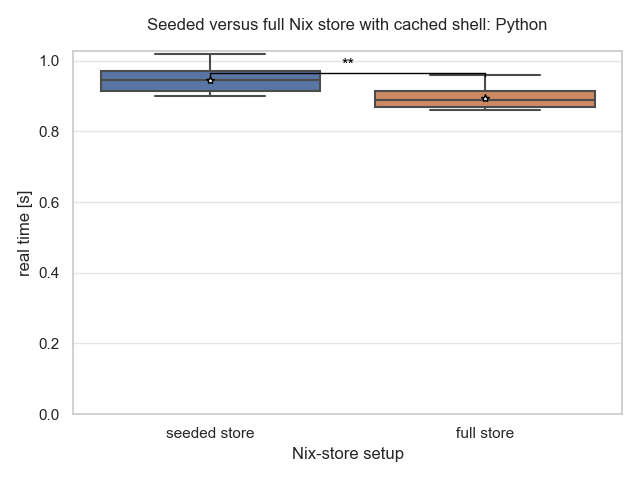
\includegraphics[width=0.75\textwidth]{thesis/graphics/nsar-plots/seeded_versus_full_nix_store_with_cached_shell:_python.png}
  \caption{The “seeded store” has a subset of the packages preinstalled to build the measured build time. The “full store” measures a subsequent build using the cached results of a first-time build with the same configuration. This graph shows the Python environment. Remarks: NSAR = nix-shell at runtime, BIAR = build image at runtime, n.s. = statistically nonsignificant difference., * = a higher number of stars(*) indicates a greater statistically significant difference.}
  \label{appendix:seeded-nix-store-python}
\end{figure}

\section{Packages included in environments for benchmarks}\label{appendix:bench-envs-packages}
The following configuration belong to the group $C_{base}$ and the specified packages are included in the benchmarks of both prototypes.
\subsection{Base packages}
\begin{lstlisting}[caption={base-pkgs.nix}, title={base-pkgs.nix}, label={base-pkgs.nix}]
{ pkgs }:
{
  inputs = with pkgs; [
    coreutils-full
    bashInteractive
    curl
  ];
}
\end{lstlisting}
\subsection{\textbf{\texttt{C++}} packages}
The Nix configuration that is used to prebuild the seeded Nix store is \nameref{cpp.nix}. 
\begin{lstlisting}[caption={cpp.nix}, title={cpp.nix}, label={cpp.nix}]
{ pkgs }:
{
  inputs = with pkgs; [
    autoconf
    automake
    bison
    flex
    binutils
    gdb
    libtool
    cmake
    strace
  ];
}
\end{lstlisting}
The Nix configuration used for benchmarking has the additional numerical library package \verb|eigen| in its configuration.

\subsection{Python packages}\label{appendix:bench-envs-packages-python}
The Nix configuration that is used to prebuild the seeded Nix store is \nameref{python.nix}. 
\begin{lstlisting}[caption={python.nix}, title={python.nix}, label={python.nix}]
{ pkgs }: with pkgs;
let
  pythonEnv = python39.withPackages (p: with p; [
    scipy
    numpy
    pandas
    termcolor
    networkx
    gnureadline
    jinja2
    matplotlib
  ]);
in
{
  inputs = [ pythonEnv ];
}
\end{lstlisting}

The Nix configuration that is used for benchmarking (see \nameref{bench-python.nix}) has \verb|scikit-learn| as an additional Python package as well as six additional OS packages compared to \nameref{python.nix}.
\begin{lstlisting}[caption={bench-python.nix}, title={bench-python.nix}, label={bench-python.nix}]
{ pkgs }: with pkgs;
let
  pythonEnv = python39.withPackages (p: with p; [
    scipy
    numpy
    pandas
    termcolor
    networkx
    gnureadline
    jinja2
    matplotlib
    
    # added Python package
    scikit-learn
  ]);
in
{
  inputs = [
    pythonEnv
    
    # added OS packages
    ncurses
    bzip2
    openssl
    sqlite
    xz
  ];
}
\end{lstlisting}

\subsection{Current approach packages}
The \verb|Python-3_8| cxEnvironment, which we used for benchmarking, has the same OS packages and Python packages as \nameref{bench-python.nix}. The \verb|GCC| configuration we used for benchmarking and comparing to our \verb|C++| environment has, apart from an additional package (\verb|eigen|), the same packages installed as \nameref{cpp.nix}. Note that the \verb|nixos/nix| base image already has the \verb|gcc| and \verb|gcc-c++| compiler installed and are therefore not in the Nix configuration. 

\backmatter

\bibliographystyle{plain}
\bibliography{refs}

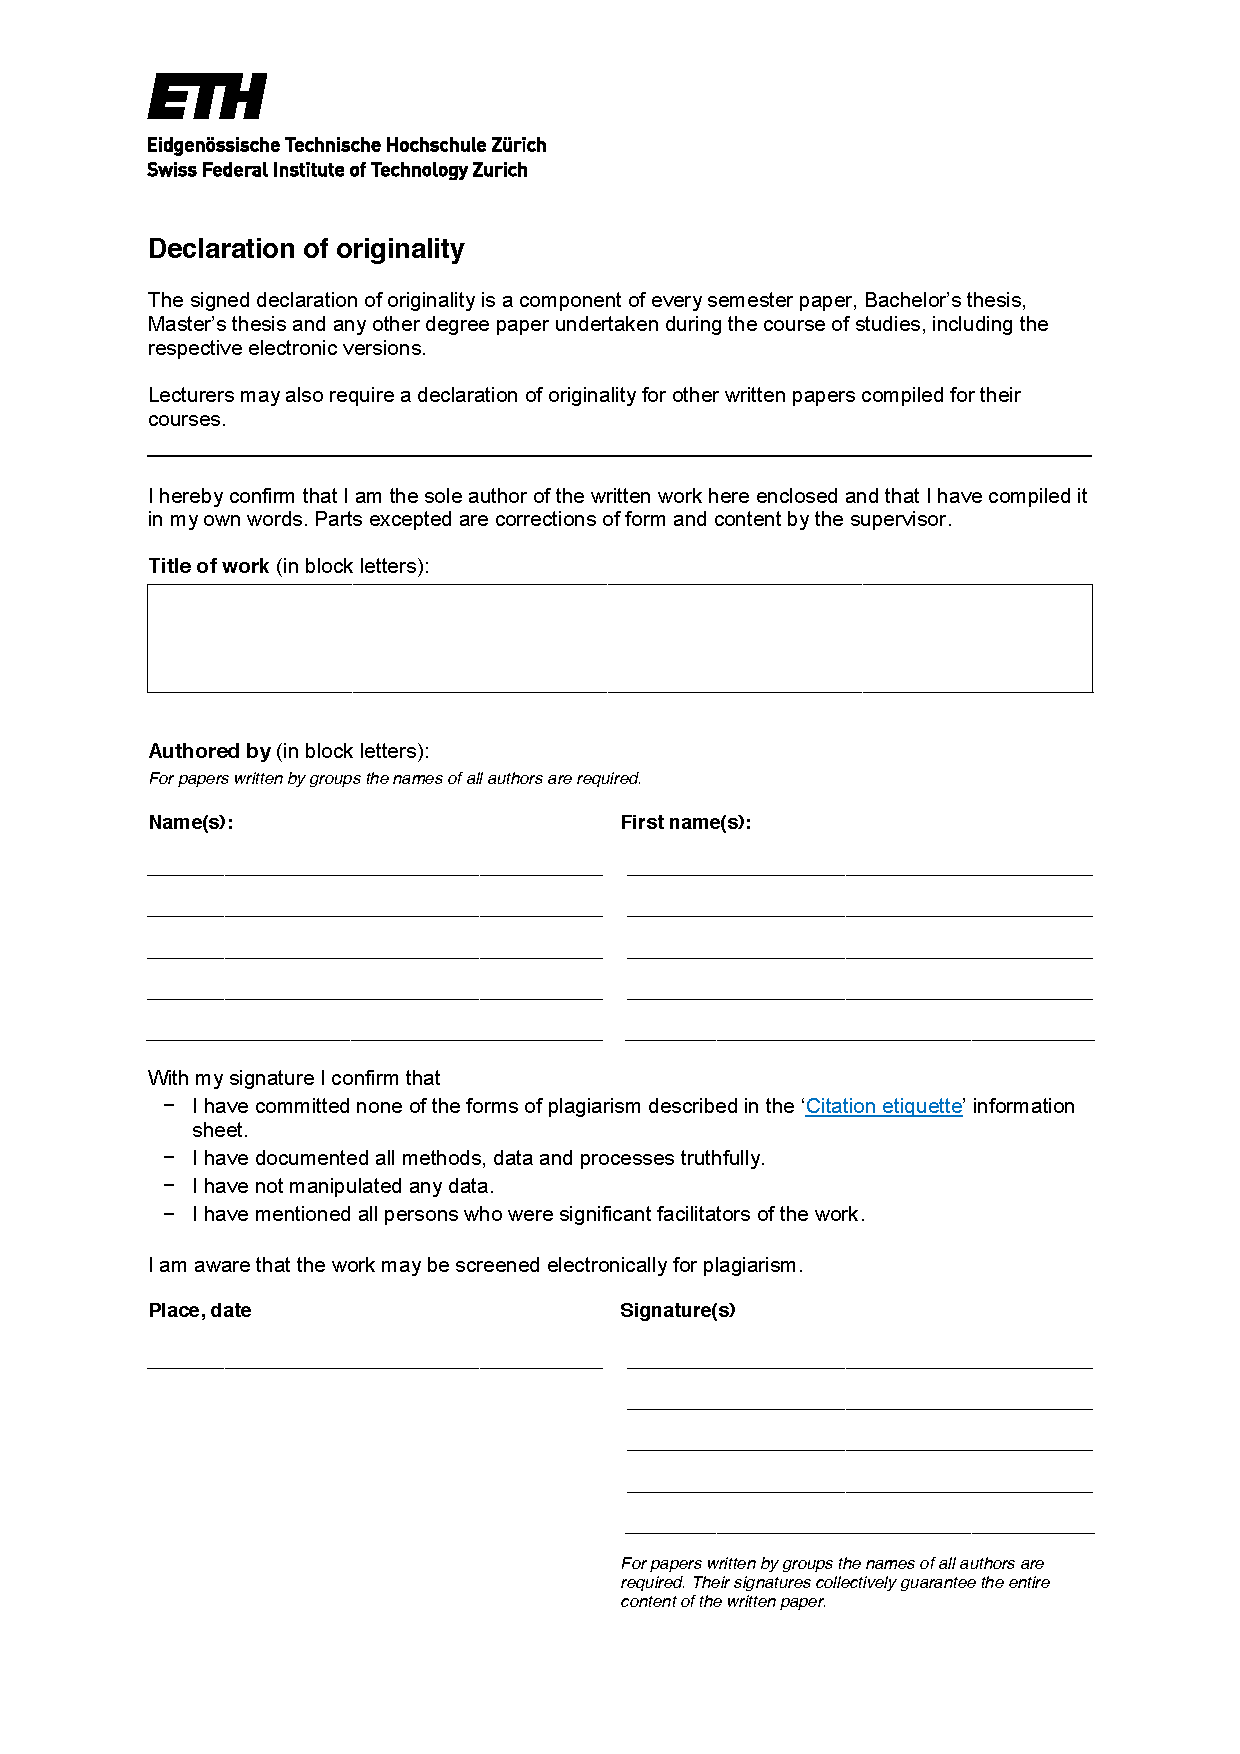
\includepdf[pages={-}]{declaration-originality.pdf}

\end{document}
